\documentclass[a4paper,oneside,12pt]{hwthesis}

%PATHDEFS
\newcommand*{\figpath}{../../include/figures}
\newcommand*{\chappath}{../../include/chapters}
\newcommand*{\refpath}{../../include/refs}

% packages
\usepackage[square,numbers,compress]{natbib}		
\usepackage{amsmath}						
\usepackage{amssymb}						
\usepackage{graphicx}
\usepackage{subfig}										
\usepackage{cleveref}					
\usepackage[section]{placeins}	
\usepackage{listings}
\usepackage{textcomp}
\usepackage[usenames,dvipsnames]{xcolor}
\usepackage[labelfont=bf]{caption}
\usepackage{pdfpages}
\usepackage{longtable}
\usepackage{tabu}

\tabulinesep=2mm

% set reference section title
\renewcommand\bibname{References}

% set subcaption crossref style
\captionsetup[subfigure]{subrefformat=simple,labelformat=simple}
    \renewcommand\thesubfigure{ (\alph{subfigure})}

\spacing{1.25}

\lstset{
	basicstyle=\ttfamily,
	language=Matlab,
	breaklines=true,
	upquote=true,
	keepspaces=true,
	showstringspaces=false,
	numbers=none,
	numbersep=5pt,
	numberstyle=\tiny\color{Gray},
	keywordstyle=\color{Blue},
	stringstyle=\color{Orchid},
	commentstyle=\color{ForestGreen}
}

% title info
\author{Oliver Thomson Brown}
\title{Stationary States of Dissipative Many-Body Quantum Systems via Matrix Product Operators}
\degree{Doctor of Philosophy in Physics}
\department{Engineering \& Physical Sciences}
\gmonth{April}
\gyear{2018}

\begin{document}

\maketitle

\pagenumbering{roman}

\begin{abstract}
In this thesis we consider stationary states of dissipative many-body quantum systems. We do so using matrix product operator representations of the system. One can find the stationary state by simulating the time evolution of the system \cite{Vidal2004,Schollwock2011}, or by using a more recently proposed variational search technique \cite{Cui2015,Mascarenhas2015}. An implementation of the variational search technique was written for MATLAB \cite{otb:gitVSSS,MATLAB}. Documentation is included in \cref{chp:mpostat}.

Using these techniques we first considered a geometrically frustrated lattice system, in which particles cannot move coherently \cite{Owen2017}. We found that local Markovian dissipation can induce mobility and long-range first-order coherence in the system. This was true in both the non-interacting and interacting regime, though strong interactions suppress the effect.

We then investigated an array of nonlinear cavities, with a coherent parametric drive to the doubly excited state \cite{Brown2018}. The dissipation rate on each site increases with the excitation number. We found that when the hopping rate between sites is low the system forms an incompressible state with commensurate filling, analogous to the Mott insulator. When the hopping rate increases there is a crossover to a delocalized state. In contrast to the equilibrium case, long-range correlations do not build up.

We conclude the thesis by considering some initial results from a new investigation, and by commenting on possible future directions for the variational stationary state search code.
\end{abstract}

\begin{acknowledgements}
First of all, I must thank my supervisor Michael Hartmann. He has been incredibly supportive, and allowed me to develop my interests in scientific software development. At times his patience has seemingly tended to infinity, particularly while reviewing this thesis! I would also like to thank my undergraduate supervisor, Sabrina Maniscalco, without whom I would never have begun my PhD. Her enthusiasm inspired me to stick with physics a little longer.

Thank you to the staff of the Condensed Matter CDT, who work extremely hard to give myself and others like me this opportunity. I am especially grateful for the generous travel funding! As anyone who has met me since I spent six weeks in California knows, I once got to spend six weeks doing research in California. I often think fondly of my time there, as I look at the wind and rain outside my window in Edinburgh. Special thanks to the present and former administrative staff of both the CDT and Heriot-Watt: Julie, Christine, Wendy, Loraine, and Sheila. It is clear that without them, nothing would ever get done.

Thank you to all my long-suffering friends, colleagues, and flatmates, present and former. All of them have helped me to enjoy Edinburgh so much that I intend to stick around for some time. Especially the lunch crew, Ash, Adam, Stuart, and James, and Darren, who introduced me to climbing. Special thank you to my friend from `back home' James Puddephatt, as he agreed to proofread my thesis in exchange for a bag of haribo. Any mistakes that still remain are certainly my fault, but I will blame him anyway.

Thank you to my grandparents, John ``Jock'' Thomson Brown, Marguerite ``Peggy'' Brown (Scotland Nan), and Brenda Sneade (Telford Nan). Without their generous support, I would never have completed even my undergraduate degree. It seems unlikely I can return the favour, so I must pass it on instead.   

Thank you to my father, Robert Andrew Brown, who first spurred my interest in computers. He is the only person I've ever met who could ramble about nothing for as long as I can. If he could, I'm sure he would read this thesis cover to cover. Finally, to my mother Rosemary Helen Brown, who is strong in ways I cannot imagine: thank you for \emph{everything}.
\end{acknowledgements}

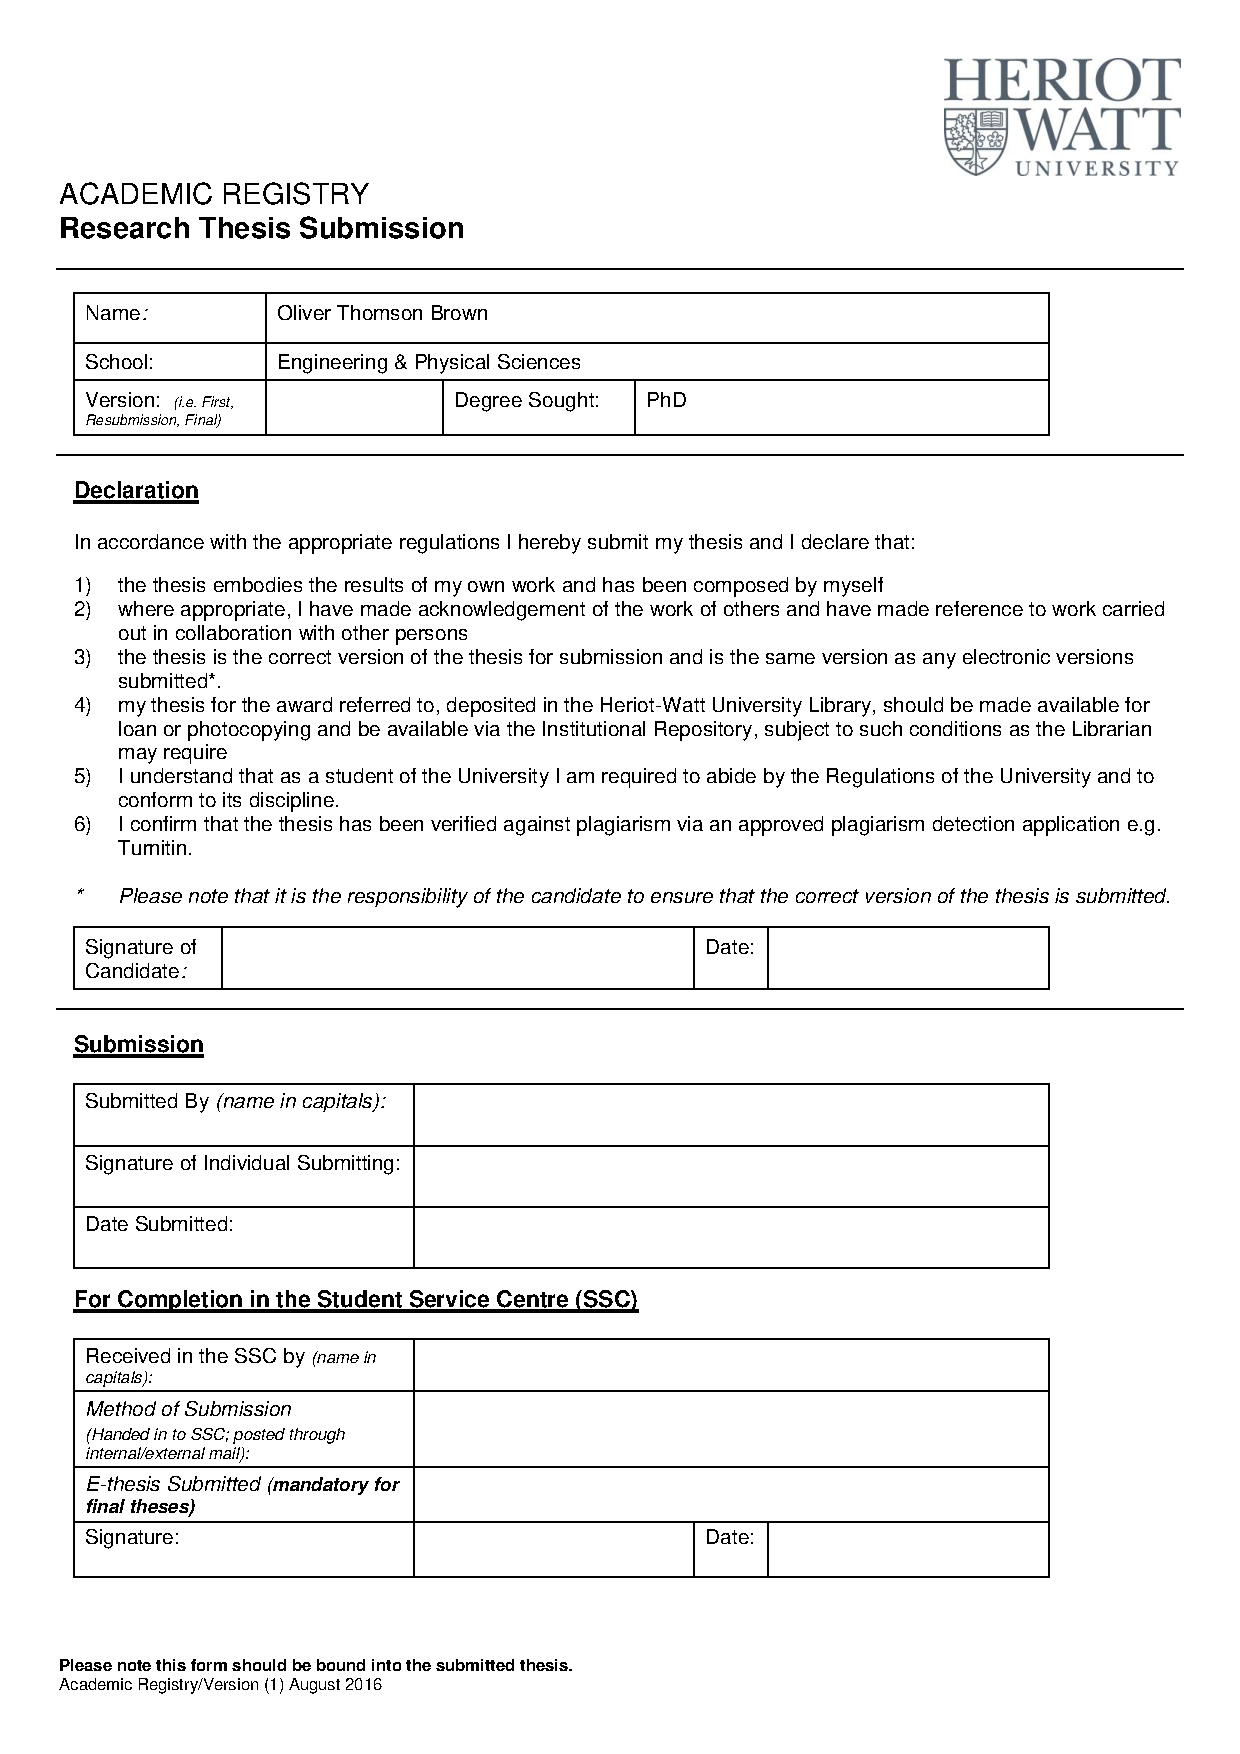
\includepdf{../../include/researchthesissubmission}

\tableofcontents

\chapter{Introduction}
\pagenumbering{arabic}
\setcounter{page}{1}

This thesis is structured in the following way. We will begin in \cref{chp:MBQOQS} by discussing many-body quantum physics, in particular the scaling problem, which makes it such a challenging field. We will then introduce a particular physical model -- the driven-dissipative Bose-Hubbard -- which we are particularly interested in investigating. We will give two examples of physical systems in which such a model can be implemented, paying particular attention to the introduction of nonlinearity and dissipation to the system. We will then introduce the basics of open quantum systems, remarking on the Lindblad-form master equation. We limit ourselves to solving for the steady state of a system under the action of Lindblad dynamics, though the relaxation of the approximations inherent to the Lindblad master equation is itself an open and very interesting field of research. Finally in this chapter, we will briefly consider the practicalities of numerically solving for the steady state. We do so as a sort of primer for the following chapter.

In \cref{chp:NM} we will begin by introducing matrix product states -- one answer to the scaling problem. MPS are a way of representing quantum states which allow for the compression of states with low levels of entanglement, which were first introduced in the form in which we use them by Guifr\'{e} Vidal \cite{Vidal2003,Vidal2004}, though they are essentially an evolution of the DMRG method due to Steven White \cite{White1992,White1993}, and the analytical matrix product states previously used to study finitely correlated states \cite{Affleck1987}. We then introduce the matrix product operator, a way of representing a Hamiltonian or, more importantly as far as we are concerned, a Liouvillian, in a similar format to the matrix product state. The MPO is critical to the variational search technique, and our work owes most to the recent efforts of Cui \cite{Cui2015} and Mascarenhas \cite{Mascarenhas2015}, who extended the variational search approach from finding the ground state of a closed system, to finding the stationary state of an open one. One of, if not \emph{the}, key outputs of my PhD is a variational stationary state search code \cite{otb:gitVSSS} which was written for Matlab \cite{MATLAB}. The documentation for that code is included in this thesis as \cref{chp:mpostat}. We also, more briefly, mention time evolution methods using matrix product states. Although powerful, the variational search technique does not work for every system. Time evolution therefore still plays an important role in research presented later in the thesis.

Next in \cref{chp:DIM} we consider the first published research of this thesis, ``Dissipation-induced mobility and coherence in frustrated lattices'' \cite{Owen2017}. Here we considered a model of a geometrically frustrated lattice system, which was coupled to a dissipative environment in such a way that dissipative transport was possible. The first half of the paper considers the non-interacting regime, which could be solved using the Ehrenfest equations, however the second half considers a strongly interacting regime. This was the first attempt we made to use the variational search code on a `real' problem, and it was successful. We determined that dissipation enabled transport through the lattice in both the non-interacting, and interacting case, although strong interaction suppressed mobility. Designing an MPO which includes so many non-local terms is a little tricky, so the full MPO is included in \cref{chp:dimmpo} along with some explanatory notes, in the hope it may prove useful to others pursuing similar investigations.

Then in \cref{chp:DNLCA} we expand on work which has been submitted though not yet published, ``Localization to delocalization crosssover in a driven nonlinear cavity array'' \cite{Brown2018}. This was the principle scientific investigation of my PhD, however, this system was not amenable to solution using the variational search technique as we had hoped it might be. Instead we made use of TEBD, a matrix product state time evolution method. This was effective, though computationally costly. We were able to determine that a parametrically driven nonlinear cavity array, with dissipation that was larger for higher numbers of excitations on a site, exhibits a localized steady state analogous to the Mott insulator when the hopping rate between sites is low. At high hopping rates, we did not observe a superfluid-like state as in the equilibrium case, as long range coherences did not build up. \Cref{chp:rotframe,chp:adelim} are technical appendices containing derivations related to this project, which were too lengthy for inclusion in the article.

In \cref{chp:FW} we look at a new project which I have done some preliminary work on, which again features non-local dissipation. It is a biased spin chain, which has already shown some interesting results regarding dissipative transport. Such a system has previously been studied as a model of a biological photocell \cite{Fruchtman2016}, however that investigation was limited to the subspace of only one excitation. We consider a similar system in the many-body context. 

Finally, in \cref{chp:Conclusion} we indulge in some conjecture as to the future direction of both that project, and of the variational search code, in order to conclude the thesis by casting our eyes forward. 

\chapter[MBQT \& OQS]{\label{chp:MBQOQS}Many-body quantum theory \& open quantum systems}

In this chapter we will consider some of the theoretical background of many-body and open quantum systems. These are rather broad field, so we shall focus in particular on aspects that are relevant to the research presented later in this thesis. We will begin by considering what is meant by an `many' in many-body quantum systems, and why this presents such a challenge to physicists. We will also briefly introduce some of the conventions from quantum optical lattice systems, in order to make later chapters more transparent. Then we will discuss what is meant by an `open' quantum systems, and consider what approximations are commonly applied in order to reduce the complexity of the problem. Finally we shall discuss how to construct a linear system of equations representing the many-body open quantum system.  

\section{Many-Body Quantum Physics}

\subsection{How many?}
Quantum physics has a problem. More than one actually, but the reader may safely assume that the author considers musing on the interpretation of quantum mechanics to be far above his pay-grade, and that he belongs to the ``Shut up and calculate!'' school of thought \cite{Mermin89}. What hardship then, does quantum mechanics present to those of us interested only in crunching numbers and getting results? 

To answer that, let us first step back and consider a classical system. Consider some system of \(N\) components, each of which can be in one of two possible states. In total there are \(2^{N}\) possible configurations of the system, each of which can be \emph{completely} described by an \(N\)-bit string. Furthermore, if we increase \(N\) to \(N+m\), we only need to add \(m\) bits. Even if we change to a system where there are three possible states of each component, although the total state space increases in size to \(3^{N}\), since the system must exist in \emph{one and only one} of those configurations, we can still efficiently represent the system with just \(N\) bits. Mathematical representations of many-body classical systems scale linearly with the size of the system (the number of `bodies'). This does not mean that classical many-body problems are \emph{easy}, just that they get harder in proportion with the size of the system.  

Enter quantum mechanics. We may again consider a system of \(N\) components, each of which can be in of two possible states, meaning there are \(2^{N}\) possible configurations -- so far, so good. However, there is a fundamental principle of quantum mechanics -- the Superposition principle -- that says that if a system may be in one of two states, which we shall label \(|0 \rangle\) and \(|1\rangle\), then it may also be in the state,
\begin{equation}
	| \psi \rangle = \alpha |0\rangle + \beta |1\rangle,
	\label{eq:mbq1-1}
\end{equation}
where \(\alpha\) and \(\beta\) are complex coefficients. This means that we must replace each of our bits with a complex vector,
\begin{equation}
	|\psi \rangle = \begin{pmatrix}
						\alpha \\
						\beta
					\end{pmatrix},
	\label{eq:mbq1-2}
\end{equation}
where we have arbitrarily chosen a convention that the first element corresponds to \(|0\rangle\), and the second to \(|1\rangle\). Still if all takes to move to the quantum many-body problems is to move from \(N\) integers to \(2N\) complex floats, this is not so bad. Unfortunately, the superposition principle applies equally to the composite system. Taking \(N=3\), if \(|\Psi\rangle = |000\rangle\) and \(|\Psi\rangle = |111\rangle\) are valid configurations, so is 
\begin{equation}  
	| \Psi \rangle = c_{000}|000 \rangle + c_{111}| 111 \rangle,
	\label{eq:mbq1-3}
\end{equation}
where \(c_{000}\) and \(c_{111}\) are again complex coefficients. In fact, any arbitrary combination of the \(2^{3} = 8\) possible states of the system,
\begin{equation}
	| \Psi \rangle = \sum^{1}_{i,j,k=0} c_{ijk} |ijk \rangle,
	\label{eq:mbq1-4}
\end{equation}
is a valid state, so we must use a vector of 8 complex values to describe the state. More generally, if we have some system of \(N\) quantum components, each of which may be in any combination of \(d\) local states, we require a state vector of \(d^{N}\) complex elements. The representation of the system grows \emph{exponentially} with its size. This scaling problem is the crux of many-body quantum physics \cite{Barnett_MS,NielsenChuang_CS}. To compound the issue, it is also clear that the properties of a many-body system are unlikely to be well predicted by single- or even few-body systems -- it has long been understood that in nature ``more is different'' \cite{Anderson72}.

\subsection{One-dimensional Lattice Systems}
Properties particular to lattice systems, and one-dimensional problems. Introduce operator notation and interaction terms. Tight-binding, Bose-Hubbard?

\subsection{Quantum Optics}
Drive and dissipation. How can we create interaction between photons, and between sites? (Many-body physics with solitons)

\section{Open Quantum Systems}

\begin{figure}[ht!]
\centering
\includegraphics[width=0.8\linewidth]{\figpath/open_system}
\caption{The canonical visual representation of an open quantum system. In open quantum systems one considers a composite system, consisting of \(S\), the \emph{system of interest}, here depicted by the blue circle, and \(E\) some well-understood environment -- here depicted by the orange ellipse. The dark blue dashed line marks the interface between the two systems. That the environment is well understood is rather crucial, and often leads to the environment itself being tightly constrained. One does not need to know the state of the environment, but it is necessary to know what states are available, and to be able to precisely define its interaction with the system of interest.}
\label{fig:oqs1-1}
\end{figure}

\chapter{\label{chp:NM}Numerical methods}

In this chapter we consider the numerical methods I have used to study the dynamics of dissipative many-body quantum systems. In particular, we consider the use of Matrix Product States to approximate the state of the system. We will first discuss the theoretical underpinnings of MPS, and then consider in detail the variational search technique. I implemented a variant of the variational search which seeks stationary states in MATLAB \cite{MATLAB}, which can be found in a repository hosted at Ref~\cite{otb:gitVSSS}. The code, named \lstinline$mpostat$, is documented in \cref{chp:mpostat}. We will then briefly discuss time evolution methods, which we have made use of in some of the published work included in this thesis. 

 \section{Matrix Product States}
 Matrix product states as we describe them here were first presented by Vidal \cite{Vidal2004}, but in effect grew from the understanding that Steven White's Density Matrix Renormalisation Group method \cite{White1992,White1993} could be reformulated to use a matrix product state representation which had previously been used as an analytical tool for finitely correlated states -- in particular the AKLT state \cite{Affleck1987}.
 Given some generic one-dimensional many-body state \(|\Psi \rangle\), we may decompose the state vector as a sum of basis vectors with individual coefficients,
 \begin{equation}
 	|\Psi \rangle = \sum_{\sigma_{1} \ldots \sigma_{N}} c_{\sigma_{1} \ldots \sigma_{N}}| \sigma_{1} \ldots \sigma_{N} \rangle,
 	\label{eq:mps1-1}
 \end{equation}
 where \(\sigma_{j}\) is the local state on site \(j\). The matrix product state further decomposes these coefficients in the following way,
 \begin{equation}
 	c_{\sigma_{1} \ldots \sigma_{N}} = A^{[1]}_{\sigma_{1}} A^{[2]}_{\sigma_{2}} \ldots A^{[N]}_{\sigma_{N}},
 	\label{eq:mps1-2}
 \end{equation}
 where each \(A^{[n]}_{\sigma}\) is a so-called matrix product state `site tensor'. The first site tensor \(A^{[1]}\) has a row vector for each physical state on the first site, the last site tensor \(A^{[N]}\) has a column vector for each physical state on the last site, and each other tensor \(A^{[n]}\) has a matrix for each physical state on the \(n^{\mathrm{th}}\) site. The product of matrices for a particular set of local states recovers the coefficient for that many-body basis vector. On the face of it, this is nothing more than a convoluted way to write state vectors. While every state vector is unique, MPS representations are degenerate as we have introduced additonal degrees of freedom in the form of the virtual dimensions (rows and columns) in each site tensor. There are two things that make this technique fundamentally useful.

 Firstly, we can limit the size of the virtual dimensions. Typically in an exact representation the virtual dimensions will grow as we move through the system reaching a maximum on the middle site(s) and then decrease again, keeping in mind the constraint that the second virtual dimension on the site \(n\) must match the size of the first virtual dimension on the site \(n+1\), and the first and last sites must be vectors. We can construct the MPS such that the virtual dimension never exceeds some value \(\chi_{\mathrm{max}}\) to create an approximation to the state, and we can further use the Singular Value Decomposition to programatically ensure that these compressed tensors are optimal. Importantly, thanks to Vidal's observation that using the SVD in this manner is equivalent to performing a Schmidt decomposition on a bipartite splitting of the state, it is clear what exactly we lose when we compress the state this way \cite{Vidal2003}. Since the number of non-zero coefficients is a measure of entanglement in the system, if we truncate our virtual dimensions by removing components with the smallest singular values, we lose access to more highly entangled states. To put it another way, MPS is a useful and efficient representation for states with low levels of entanglement. At the extreme end, a product state could be represented with a virtual dimension of 1 on every site.

 Secondly, we can perform useful operations on individual site tensors. A tensor network can be constructed which when contracted yields the result of some operator acting on the matrix product state. Furthermore, expectation values can be calculated by introducing the conjugate matrix product state \cite{Schollwock2011,Orus2014}. This allows us to efficiently investigate the system represented by the MPS, as long as we do not require representation of a state with more entanglement than compression allows. One example of this which we shall discuss in great detail is the variational search, in which individual site tensors are optimised with respect to some operator such as a Hamiltonian or Liouvillian \cite{Verstraete2004,Cui2015}. One can also efficiently perform time evolution of the state, and indeed this was the first method developed explicitly using MPS, being familiar from DMRG \cite{Vidal2004}.

 Key to some of these techniques is the ability to represent operators in a similar way. We shall discuss Matrix Product Operators (MPOs) next.

 \section{Matrix Product Representation of Operators}
 In order to make effective use of matrix product states it is helpful to write operators in a compatible format. This is achieved through the matrix product operator formalism, however, MPOs must, in general, be constructed by hand \cite{McCulloch2007,Crosswhite2008,Frowis2010,Pirvu2010,Schollwock2011}. Note that when I refer to MPOs throughout this thesis I mean matrix product representations of operators such as the Hamiltonian, Liouvillian, or observables. The distinction is necessary as the matrix product representation of a density matrix is also a matrix product operator by dint of having both input and output states. I will refer to an MPO representation of a density matrix as a Density Matrix Product Operator (DMPO), in order to distinguish it.

 We will now discuss the process of constructing an MPO, beginning with the following simple one-dimensional Heisenberg XXX model with open boundary conditions,
 \begin{equation}
 	\mathcal {H} = -J \sum_{j=1}^{N-1} \left[ \sigma^{x}_{j}\sigma^{x}_{j+1} + \sigma^{y}_{j}\sigma^{y}_{j+1} + \sigma^{z}_{j}\sigma^{z}_{j+1} \right] - h \sum_{j=1}^{N} \hat{\sigma}^{z}_{j},
 	\label{eq:mpo1-1}
 \end{equation}
 where \(\sigma^{x,y,z}\) are the spin Pauli matrices, \(J\) is a coupling constant, and \(h\) is an external field. We recall the fact that the notation \(\sigma^{x}_{j}\) is a short hand which in fact refers to the tensor product,
 \begin{equation*}
 	\cdots \mathbb{I} \otimes \mathbb{I} \otimes \sigma^{x} \otimes \mathbb{I} \otimes \mathbb{I} \cdots
 \end{equation*}
 where the \(\sigma^{x}\) is the \(j^{\mathrm{th}}\) operator in the chain. Keeping that in mind, our MPO matrices should deliver chains of operators of the form,
 \begin{equation*}
 	\cdots \mathbb{I} \otimes -h\sigma^{z} \otimes \mathbb{I} \cdots
 \end{equation*}
 and
 \begin{equation*}
 	\cdots \mathbb{I} \otimes -J\sigma^{x,y,z} \otimes \sigma^{x,y,z} \otimes \mathbb{I} \cdots
 \end{equation*}
 for each site. Additionally, as with the MPS, the first site MPO tensor should be a row vector, and the last site MPO tensor should be a column vector. Since the Hamiltonian is homogeneous across all sites in the bulk, the same MPO tensor can be used for each. One valid formulation then is,
 \begin{align}
 	H^{[1]} &= \begin{bmatrix} -h\sigma^{z} & -J\sigma^{x} & -J\sigma^{y} & -J\sigma^{z} & \mathbb{I} \end{bmatrix}, \label{eq:mpo1-2} \\
 	H^{[\mathrm{bulk}]} &= \begin{bmatrix} \mathbb{I} & 0 & 0 & 0 & 0 \\
 										   \sigma^{x} & 0 & 0 & 0 & 0 \\
 										   \sigma^{y} & 0 & 0 & 0 & 0 \\
 										   \sigma^{z} & 0 & 0 & 0 & 0 \\
 										    -h\sigma^{z} & -J\sigma^{x} & -J\sigma^{y} & -J\sigma^{z} & \mathbb{I}
 							\end{bmatrix}, \label{eq:mpo1-3} \\
 	H^{[N]} &= \begin{bmatrix} \mathbb{I} \\ \sigma^{x} \\ \sigma^{y} \\ \sigma^{z} \\ -h\sigma^{z} \end{bmatrix}, \label{eq:mpo1-4}
 \end{align}
 which in the simplest, three-site case yields,
 \begin{align}
 	&H^{[1]}H^{[2]}H^{[3]} \notag \\
 	&= \begin{bmatrix} -h\sigma^{z}, & -J\sigma^{x}, & -J\sigma^{y}, & -J\sigma^{z}, & \mathbb{I} \end{bmatrix} \notag \\
 	&\qquad \times
 							\begin{bmatrix} \mathbb{I} & 0 & 0 & 0 & 0 \\
 										   \sigma^{x} & 0 & 0 & 0 & 0 \\
 										   \sigma^{y} & 0 & 0 & 0 & 0 \\
 										   \sigma^{z} & 0 & 0 & 0 & 0 \\
 										    -h\sigma^{z} & -J\sigma^{x} & -J\sigma^{y} & -J\sigma^{z} & \mathbb{I}
 							\end{bmatrix}
 							\begin{bmatrix} \mathbb{I} \\ \sigma^{x} \\ \sigma^{y} \\ \sigma^{z} \\ -h\sigma^{z} \end{bmatrix}, \notag \\
 	&= \begin{bmatrix} (-h\sigma^{z}\mathbb{I} - J\sigma^{x}\sigma^{x} - J\sigma^{y}\sigma^{y} - J\sigma^{z}\sigma^{z} - h\mathbb{I}\sigma^{z}), & -J\mathbb{I}\sigma^{x}, & -J\mathbb{I}\sigma^{y}, & -J\mathbb{I}\sigma^{z}, & \mathbb{I}\mathbb{I} \end{bmatrix} \notag \\
 	&\qquad \times \begin{bmatrix} \mathbb{I} \\ \sigma^{x} \\ \sigma^{y} \\ \sigma^{z} \\ -h\sigma^{z} \end{bmatrix}, \notag \\
 	&= -h\sigma^{z}\mathbb{I}\mathbb{I} - J\sigma^{x}\sigma^{x}\mathbb{I} - J\sigma^{y}\sigma^{y}\mathbb{I} - J\sigma^{z}\sigma^{z}\mathbb{I} - h\mathbb{I}\sigma^{z}\mathbb{I} - J \mathbb{I}\sigma^{x}\sigma^{x} -  J \mathbb{I}\sigma^{y}\sigma^{y} \notag \\
 	&\qquad - J \mathbb{I}\sigma^{z}\sigma^{z} - h \mathbb{I}\mathbb{I}\sigma^{z},
 	\label{eq:mpo1-5}
 \end{align}
 which is indeed correct. How exactly the physical and virtual dimensions are arranged after this point is an implementation detail, which we need not concern ourselves with at the design stage. It should be noted that this formulation is not unique, but we have chosen certain conventions, such as scalar coefficients being included in the `leading' terms, and making use of the bottom row and first column in the bulk MPO. Obviously, more complex Hamiltonians require more complex MPOs -- in particular moving beyond nearest-neighbour coupling requires making use of the inner space in the bulk MPO, and the creation of `passing lanes' in the main row and column. We defer further discussion of that until later when we discuss Ref.~\cite{Owen2017}, which relied heavily on such techniques.

 We will now briefly discuss the additional complexity involved in creating an MPO for a Liouvillian, as this is directly useful for the variational stationary state code presented later. Firstly, we note that \(|\rho (\mathbf{x}) \rangle \rangle\) denotes the density matrix vectorised according to the isomorphism,
\begin{align}
\rho &= \sum_{ij} c_{ij} |i \rangle \langle j| \notag \\
\rightarrow | \rho \rangle \rangle &= \sum_{ij} c_{ij} |j \rangle \otimes |i \rangle,
\label{eq:vs1-11}
\end{align}
where \(|i\rangle\) is some complete set of basis states. Second, we note that formation of the Liouvillian matrix, \(\hat{\mathcal{L}}\) which acts on the vectorised density matrix, \(|\rho \rangle \rangle\) relies on the following property. Given the matrix equation,
 \begin{equation}
 	AXB = C,
 	\label{eq:mpo1-6}
 \end{equation}
 one can write,
 \begin{equation}
 	(B^{T} \otimes A)\vec{X} = \vec{C}.
 	\label{eq:mpo1-7}
 \end{equation}
 Given then that the system dynamics are given by \(\dot{\rho} = -i[\mathcal{H}, \rho]\), we must write an MPO form of the equation,
 \begin{equation}
 	\hat{\mathcal{L}}|\rho \rangle \rangle = \left( \mathbb{I} \otimes -i\mathcal{H} + i\mathcal{H}^{T} \otimes \mathbb{I} \right)| \rho \rangle \rangle.
 	\label{eq:mpo1-8}
 \end{equation}
 The additional complexity in the MPO structure is clear -- we must account separately for terms on the `left' and `right' side of the tensor product. As an example we consider the bulk MPO for the dynamics of our one-dimensional Heisenberg XXX system \cref{eq:mpo1-1}. It is as follows,
 \begin{align}
 	&\hat{\mathcal{L}}^{\mathrm{bulk}} = \notag \\
 	&\resizebox{0.98\linewidth}{!}{%
 	\(\begin{bmatrix}
 		\mathbb{I} \otimes \mathbb{I} & 0 & 0 & 0 & 0 & 0 & 0 & 0 \\
 		\mathbb{I} \otimes \sigma^{x} & 0 & 0 & 0 & 0 & 0 & 0 & 0 \\
 		\sigma^{x} \otimes \mathbb{I} & 0 & 0 & 0 & 0 & 0 & 0 & 0 \\
 		\mathbb{I} \otimes \sigma^{y} & 0 & 0 & 0 & 0 & 0 & 0 & 0 \\
 		\sigma^{yT} \otimes \mathbb{I} & 0 & 0 & 0 & 0 & 0 & 0 & 0 \\
 		\mathbb{I} \otimes \sigma^{z} & 0 & 0 & 0 & 0 & 0 & 0 & 0 \\
 		\sigma^{z} \otimes \mathbb{I} & 0 & 0 & 0 & 0 & 0 & 0 & 0 \\
 		\mathbb{I} \otimes ih\sigma^{z} - ih\sigma^{z} \otimes \mathbb{I} & \mathbb{I} \otimes iJ\sigma^{x} & -iJ\sigma^{x} \otimes \mathbb{I} & \mathbb{I} \otimes iJ\sigma^{y} & -iJ\sigma^{yT} \otimes \mathbb{I} & \mathbb{I} \otimes iJ\sigma^{z} & -iJ\sigma^{z} \otimes \mathbb{I} & \mathbb{I} \otimes \mathbb{I}
 	\end{bmatrix},\)}
 	\label{eq:mpo1-9}
 \end{align}
 an essentially trivial extension of the Hamiltonian MPO, however care must be taken over minus signs, and note that \(\sigma^{xT} = \sigma^{x}, \sigma^{zT} = \sigma^{z},\) but \(\sigma^{yT} \neq \sigma^{y}\). The precise arrangement of the virtual and physical dimensions is again an implementation dependent detail, but note that we here have again two virtual dimensions (rows and columns), but four physical dimensions.

 Having described matrix product states and operators in a general sense, we will now discuss one particular technique which makes use of them -- the variational search procedure.

 \section{Variational Search}
 It is well known that one can use the Rayleigh-Ritz Variational Technique to find an approximation to the lowest eigenvalue and corresponding eigenfunction of a Hermitian operator. Given a set of variational parameters upon which the eigenfunctions depend, one can move always to a lower eigenvalue, by minimising over one parameter at a time \cite{ArfWeb_RRVT, Gasiorowicz_RVT}. Consequently, we can find an approximation to the ground state of a system by minimising the expression,
\begin{equation}
E = \frac{\langle \psi (\mathbf{x}^{*}) | \hat{H} | \psi (\mathbf{x}) \rangle}{\langle \psi (\mathbf{x}^{*}) | \psi (\mathbf{x}) \rangle},
\label{eq:vs1-1}
\end{equation}
with respect to some \(x\), where E is the energy of the system, \(\hat{H}\) is a Hamiltonian, \(\psi\) is an approximation to the ground state, and \( \mathbf{x} \) is a set of \emph{variational parameters}. Equally, we can find an approximation to the stationary state of an open quantum system by minimising the expression,
\begin{equation}
\frac{\mathrm{d}}{\mathrm{d}t}\langle \langle \rho|\rho \rangle \rangle = \langle \langle \rho(\mathbf{x}^{*}) | \hat{\mathcal{L}^{\dagger}} \hat{\mathcal{L}} | \rho(\mathbf{x}) \rangle \rangle,
\label{eq:vs1-2}
\end{equation}
with respect to some \(x\), where \(\hat{\mathcal{L}}\) is a Liouvillian matrix, \(\rho\) is an approximation to the stationary state, and \(\mathbf{x}\) is again some set of variational parameters. We will discuss here the generic case in which we have some observable \(O\) we wish to minimise, which has an operator \(\hat{O}\). As such we seek to use matrix product states to minimise the expression,
\begin{equation}
\langle \psi(\mathbf{x}^{*}) | \hat{O} | \psi(\mathbf{x}) \rangle,
\label{eq:vs1-10}
\end{equation}
with respect to some \(x\). A visual representation of the variational search procedure is provided in \cref{fig:vs1-1}.

\begin{figure}[ht!]
\centering
\includegraphics[width=0.9\linewidth]{\figpath/var_space}
\caption{A visual representation of a variational search using matrix product states. The purple background represents the total state space of the system, and the green oval is the part of that state space that can be represented by a matrix product state of some finite dimension. The orange star represents our desired solution state, and in this case it is inaccessible to the matrix product state space. The black circle is the initial matrix product state, the black star is the nearest matrix product state approximation to the solution state, and the black squares are states through which the matrix product state transitions on its way to the solution state. The black dashed line represents a variational step -- an optimisation over one or more of the variational parameters. The transitional states may or may not have some physical meaning in the context of the variational search depending on the specifics of the system being investigated. In general, however, if one wishes to know \emph{how} a system reaches the solution state a time evolution method should be used, not a variational search.}
\label{fig:vs1-1}
\end{figure}

When using matrix product states the set of variational parameters we employ are the individual site tensors, \(A^{[n]}\). We shall discuss the search procedure as prescribed by Ulrich Schollw\"{o}ck's excellent review article \cite{Schollwock2011}. I begin my explanation by assuming that we have already some initial matrix product state, \(\Psi_{\mathrm{init}}\) which is normalised according to the vector norm, and has dimensions \(N \times \chi_{j-1} \times \chi_{j} \times d\), where \(N\) is the number of sites in the system, \(d\) is the local state space dimension, \(\chi_{j}\) is the local virtual dimension and meets the condition \(\chi_{j} \leq \chi_{\mathrm{max}}\), which is the maximal allowed virtual dimension. Additionally I assume we may represent the operator \(\hat{O}\) as a matrix product operator with site tensors \(O^{[n]}\). First, we construct left and right `blocks' for each site in the system. The left block for some site \(n\) is a rank-3 tensor which contains the expectation of \(\hat{O}\) from the first site up to the site \(n-1\). The right block for some site \(n\) is a rank-3 tensor which contains the expectation of \(\hat{O}\) from the last site through to the site \(n+1\). This is shown diagramatically in \cref{fig:vs1-2}.

\begin{figure}[ht!]
\centering
\includegraphics[width=0.9\linewidth]{\figpath/LR_blocks}
\caption{A tensor network diagram for a system which has been partially contracted in order to form left and right blocks, \(L^{[n]}\) and \(R^{[n]}\). The upper red dot here is a tensor for the site \(n\), \(A^{[n]}\), and the lower red dot is its conjugate, \(A^{\dagger [n]}\). The blue square is the mpo tensor \(O^{[n]}\) of some observable with an operator \(\hat{O}\). The black lines represent tensor indices which can be contracted over. If this contraction is completed it will be equivalent to a contraction over the full system, and the result will be the expectation value \(\langle \Psi | \hat{O} | \Psi \rangle \).}
\label{fig:vs1-2}
\end{figure}

The first site left block tensor \(L^{[1]}\) is just the scalar \(1\), as there are obviously no sites before the first. The second left block tensor \(L^{[2]}\) is then found by performing the contraction procedure,
\begin{equation}
L^{[2]}_{r^{\prime}, c, q} = \sum_{\sigma^{\prime}, c^{\prime}} A^{\dagger [1] \sigma^{\prime}}_{r^{\prime}, c^{\prime}} \left( \sum_{\sigma, p} O^{[1]  \sigma, \sigma^{\prime}}_{p, q} \left( \sum_{r} A^{[1] \sigma}_{r, c} \right) \right),
\label{eq:vs1-3}
\end{equation}
where \(A^{[n]}\) is the matrix product state tensor for the site \(n\), \(\sigma\) indexes the local physical state, \(r\) and \(c\) (`row' and `column') index the local virtual dimensions, primed indices relate to the conjugate matrix product state tensor \(A^{\dagger [n]}\), and \(p\) and \(q\) index the virtual dimensions of the matrix product operator. The procedure continues from there, much as you might expect, by moving on to the third site and so on until the last site is reached. The general formula for \(L^{[n]}\) is,
\begin{equation}
L^{[n]}_{r^{\prime}, c, q} = \sum_{\sigma^{\prime}, c^{\prime}} A^{\dagger [n-1] \sigma^{\prime}}_{r^{\prime}, c^{\prime}} \left( \sum_{\sigma, p} O^{[n-1]  \sigma, \sigma^{\prime}}_{p, q} \left( \sum_{r} L^{[n-1]}_{c^{\prime}, r, p} A^{[n-1] \sigma}_{r, c} \right) \right),
\label{eq:vs1-4}
\end{equation}
which is shown diagramatically in \cref{fig:vsTMP}.

\begin{figure}[ht!]
\centering
\includegraphics[width=0.49\linewidth]{\figpath/L_contract}
\caption{A tensor network diagram which, when contracted, yields the `left block' for the site \(n\), \(L^{[n]}\). This is the operation described in \cref{eq:vs1-4}. The un-contracted indices \(c\), \(q\), and \(r'\), form the three dimensions of \(L^{[n]}\).}
\label{fig:vsTMP}
\end{figure}

The procedure for forming the right block is naturally very similar, starting from the last site with \(R^{[N]} = 1\) and,
\begin{equation}
R^{[n]}_{c^{\prime}, r, p} = \sum_{\sigma^{\prime}, r^{\prime}} A^{\dagger [n+1] \sigma^{\prime}}_{r^{\prime}, c^{\prime}} \left( \sum_{\sigma, q} O^{[n+1] \sigma, \sigma^{\prime}}_{p, q} \left( \sum_{c} R^{[n+1]}_{r^{\prime}, c, q} A^{[n+1] \sigma}_{r, c} \right) \right).
\label{eq:vs1-5}
\end{equation}
Once we have formed these left and right blocks at each site, we move on to the variational procedure proper.

We will sweep backwards and forwards through the system, updating each site tensor to minimise the energy of the overall state. Referring back to \cref{eq:vs1-1} we can see that it can be minimised by being rephrased as an eigenvalue problem,
\begin{align}
\frac{\langle \psi(\mathbf{x}^{*}) | \hat{H} | \psi(\mathbf{x}) \rangle}{\langle \psi(\mathbf{x}^{*}) | \psi(\mathbf{x}) \rangle } &= E, \notag \\
\Rightarrow \langle \psi(\mathbf{x}^{*}) | \hat{H} | \psi(\mathbf{x}) \rangle &= E \langle \psi(\mathbf{x}^{*}) | \psi(\mathbf{x}) \rangle, \notag \\
\Rightarrow \frac{\mathrm{d}}{\mathrm{d}\langle \psi(\mathbf{x}^{*}) |} \left( \langle \psi(\mathbf{x}^{*}) | \hat{H} | \psi(\mathbf{x}) \rangle \right) &= \frac{\mathrm{d}}{\mathrm{d}\langle \psi(\mathbf{x}^{*}) |} \left(  E \langle \psi(\mathbf{x}^{*}) | \psi(\mathbf{x}) \rangle \right), \notag \\
\Rightarrow \hat{H} |\psi(\mathbf{x}) \rangle &= E | \psi(\mathbf{x}) \rangle,
\label{eq:vs1-6}
\end{align}
which of course is an expression of the time-independent Schr\"{o}dinger equation. If we could solve that for the full many-body state \(| \psi (\mathbf{x}) \rangle\) then we would not need matrix product states at all. Unfortunately, we cannot -- the computational effort scales exponentially with the system size as the Hamiltonian has \(d^{2N}\) elements for a system with \(d\) local states, and \(N\) sites. What matrix product states allow us to do is to form an effective Hamiltonian for some particular \(| \psi(x) \rangle\), and instead solve the more limited eigenvalue problem,
\begin{equation}
\hat{H}_{\mathrm{eff}} |\psi(x) \rangle = E_{[x]} |\psi(x) \rangle,
\label{eq:vs1-7}
\end{equation}
from which we simply select \(|\psi(x) \rangle\) which corresponds to the lowest real value of \(E_{[x]}\). In our case \(|\psi(x) \rangle\) is \(A^{[n]}\), and \(\hat{H}_{\mathrm{eff}}\) is formed by the contraction of the \emph{environment} of \(A^{[n]}\) \cite{Orus2014}. That is we calculate,
\begin{equation}
\hat{H}_{\mathrm{eff}}^{[n]} = \langle \psi(\tilde{\mathbf{x}}) | \hat{H} | \psi(\tilde{\mathbf{x}}) \rangle,
\label{eq:vs1-8}
\end{equation}
where \(|\psi(\tilde{\mathbf{x}}) \rangle \) is our matrix product state \emph{excluding the tensor for the site \(n\)}. Such a contraction is shown diagramatically in \cref{fig:vs1-4}. Mathematically, the contraction is performed as,
\begin{equation}
\hat{H}^{[n]\, \mathrm{eff}}_{r,c,r^{\prime},c^{\prime},\sigma,\sigma^{\prime}} = \sum_{p,q} L^{[n]}_{r,r^{\prime},p} O^{[n] \sigma, \sigma^{\prime}}_{p,q} R^{[n]}_{c,c^{\prime},q},
\label{eq:vs1-9}
\end{equation}
which seems simple enough, and indeed would be except that we have an eigenvalue problem to solve. As such we require \(\hat{H}_{\mathrm{eff}}^{[n]}\) to be a matrix, not a rank-6 tensor. This can be accomplished by joining the indices corresponding to the matrix product state, and joining those of its conjugate to form a matrix \(\hat{H}^{[n]\, \mathrm{eff}}_{(\sigma ,r,c), (\sigma^{\prime},r^{\prime},c^{\prime})}\). Once this is achieved it is a simple matter of finding the eigenvector of \(\hat{H}^{[n]\, \mathrm{eff}}_{(\sigma ,r,c), (\sigma^{\prime},r^{\prime},c^{\prime})}\) corresponding to the optimal eigenvalue. Which eigenvalue depends explicitly on the problem you are trying to solve, and the eigenspectrum of the relevant operator -- some examples are given in \cref{tab:vs1-1}.
\begin{table}[h!]
	\centering
	\begin{tabu} to \linewidth{l | c | c | c}
		Problem & Operator & Eigenspectrum & Optimal Eigenvalue \\ \hline
		Ground state & Hamiltonian, \(\hat{H}\) & \(\lambda\in\mathbb{R}\) & min(\(\lambda\)) \\
		Stationary state & Liouvillian, \(\hat{\mathcal{L}}\) & \(\lambda = a + ib\) & max(Re(\(\lambda\))) \\
		 & & \(\{a \in \mathbb{R}^{-}, b \in \mathbb{R}\}\) & \\
		Stationary state & \(\hat{\mathcal{L}}^{\dagger}\hat{\mathcal{L}}\) & \(\lambda \in \mathbb{R}^{+}\) & min(\(\lambda\))
	\end{tabu}
	\caption{Examples of appropriate optimal eigenvalues for different variational problems.}
	\label{tab:vs1-1}
\end{table}

This eigenvector is the vectorised site tensor \(A^{[n]}_{(\sigma, r, c)}\), which we reshape to be \(A^{[n] \sigma}_{r,c}\) and use to update our matrix product state. Given that, it should be clear that the size of the effective Hamiltonian is dependent on the local virtual dimensions. If the maximum size of the virtual dimensions is \(\chi_{\mathrm{max}}\), then the effective Hamiltonian has at most \(\chi_{\mathrm{max}}^{4}d^{2}\) elements, which is certain to be less than \(d^{2N}\) provided \(\chi_{\mathrm{max}} < d^{\frac{1}{2}(N-1)}\). It should come as no surprise that \(\chi_{\mathrm{max}} \geq d^{\frac{1}{2}(N-1)}\) is also the condition for a guaranteed exact MPS representation. Consider that an MPS tensor with square matrices for each physical state, and \(\chi = d^{\frac{1}{2}(N-1)}\) has \(d^{\frac{1}{2}(N-1)} \times d^{\frac{1}{2}(N-1)} \times d = d^{N}\) elements.

We update the first site in our system, and must then re-normalise the site. Note that computationally, the appropriate norm for a matrix product state is the vector norm,
\begin{equation}
	\langle \psi(\mathbf{x}^{*}) | \psi(\mathbf{x}) \rangle = 1,
	\label{eq:vs1-12}
\end{equation}
regardless of the physical system being represented. For ground state searches this is no issue since the vector norm is also the appropriate measure for state vectors, however for density matrices the appropriate norm is the trace norm -- the vector norm must nevertheless be maintained to prevent numerical problems. The physically relevant trace norm condition,
\begin{equation}
	\mathrm{Tr}[\rho] = 1,
	\label{eq:vs1-13}
\end{equation}
must be separately enforced (often by simply rescaling at the end of a calculation). In principle, one could recalculate the vector norm after every update and rescale the newly updated site in order to maintain the vector norm, however this is computationally costly, requiring a contraction through the full system. A smarter approach is to begin with an appropriately normalised MPS, and to use the singular value decomposition to maintain this normalisation. The SVD decomposes some matrix \(M\) in the following way,
\begin{equation}
	M = U S V^{\dagger},
	\label{eq:vs1-14}
\end{equation}
where \(S\) is a diagonal matrix of singular values, and \(U\) and \(V\) are unitary matrices. We reshape our updated site tensor \(A^{[n] \sigma}_{r,c}\) into a matrix by joining the physical indices to the first virtual index (the \emph{rows}), and performing the SVD procedure on it. The first unitary matrix \(U\) is retained and reshaped to (once again) replace the site tensor. The singular value matrix and the second unitary are multiplied together, and then the product \(SV^{\dagger}\) is multiplied into the following site site tensor \(A^{[n+1] \sigma}_{r,c}\). This procedure ensures that normalisation is maintained throughout the system, and prevents large differences in scale between site tensors, which would cause numerical problems. That said, there is clearly a directionality to this procedure -- the reverse procedure is to retain the second unitary \(V^{\dagger}\), and to multiply \(US\) into the site site tensor \(A^{[n-1] \sigma}_{r,c}\). We therefore refer to site tensors as either left or right `canonical', and we ensure that all sites left of the update site are left-canonical, and all sites right of the update site are right-canonical. Finally we note that in a sense, this procedure `pushes' the normalisation of the MPS through the system. Consequently, if the system is made left-canonical up to the last site (or right-canonical up to the first), then performing the canonisation procedure on the last (first) site yields a single non-zero singular value, which is the vector norm of the state.

Having performed the full update and renormalisation procedure on the first site, we then update the left block tensor for the second site in the system, \(L^{[2]}\) using \cref{eq:vs1-4}. We are then ready to find an effective Hamiltonian for the second site and update it. This procedure repeats sweeping `right' through our system until we reach and update the \(N\)th site -- at this point we have updated every site in the system, but it is unlikely that our observable has converged after only one such sweep. The procedure for sweeping `left' through the system back to the first site is very similar, except when re-normalising we make our newly updated site right-canonical and then update the right block, \(R^{[n]}\). In this way we are always using the most up-to-date version of the system when we calculate the effective operator for a given site. The whole procedure repeats, sweeping left and right through the system until our chosen observable converges.

\begin{figure}[ht!]
\centering
\includegraphics[width=0.9\linewidth]{\figpath/effH_diagram}
\caption{A diagrammatic representation of the contraction that must be performed in order to find the effective operator on some site \(n\). As usual the red circles represent matrix product state tensors, the blue squares represent some matrix product operator, and black lines are indices. The lines which reach into the gap left by the missing site \(n\) are indices which are left free, and will become the indices of the effective operator. As such, it can be seen that the effective operator will be a rank-6 tensor.}
\label{fig:vs1-4}
\end{figure}

\section{Time evolution}
Although the code written by myself implements the variational stationary state search, results included in this thesis [arXiv:1709.02165] were calculated using time evolution. As such, we will briefly discuss how a matrix product state can be time evolved, specifically using the Time Evolving Block Decimation (TEBD) method due to Vidal \cite{Vidal2003}.

First of all note that in TEBD we do not use an MPO, but instead split the Hamiltonian into commuting terms. For the sake of this explanation, we shall assume that the Hamiltonian only has nearest-neighbour interactions, and can therefore be written as a sum of terms on odd and even sites,
\begin{equation}
	\mathcal{H} = \mathcal{H}_{\mathrm{odd}} + \mathcal{H}_{\mathrm{even}},
	\label{eq:te1}
\end{equation}
where importantly, the following commutation relations hold,
\begin{align}
	\left[\mathcal{H}_{\mathrm{odd}}, \mathcal{H}_{\mathrm{odd}}\right] &= 0, \label{eq:te2} \\
	\left[\mathcal{H}_{\mathrm{even}}, \mathcal{H}_{\mathrm{even}}\right] &= 0. \label{eq:te3}
\end{align}
We can then make use of the Suzuki-Trotter expansion \cite{Suzuki1976} which in general is,
\begin{equation}
	\mathrm{e}^{A+B} = \lim_{n \rightarrow \infty}\left[ \mathrm{e}^{\frac{A}{n}} \mathrm{e}^{\frac{B}{n}}\right]^{n},
	\label{eq:te4}
\end{equation}
and which allows us to expand (to first order) the time evolution over some time-step \(\tau\),
\begin{align}
	|\psi(t+\tau)\rangle &= \mathrm{e}^{-i\mathcal{H}\tau}|\psi(t) \rangle, \notag \\
	&= \mathrm{e}^{-i\mathcal{H}_{\mathrm{odd}}\tau}\mathrm{e}^{-i\mathcal{H}_{\mathrm{even}}\tau}|\psi(t) \rangle + \mathcal{O}(\tau^{2}).
	\label{eq:te5}
\end{align}
In fact, it is more conventional to use the second-order expansion,
\begin{equation}
	\mathrm{e}^{-i\mathcal{H}\tau} = \mathrm{e}^{-i\mathcal{H}_{\mathrm{odd}}\tau / 2}\mathrm{e}^{-i\mathcal{H}_{\mathrm{even}}\tau}\mathrm{e}^{-i\mathcal{H}_{\mathrm{odd}}\tau / 2} + \mathcal{O}(\tau^{3}),
	\label{eq:te6}
\end{equation}
which provides additional precision for little extra computational effort \cite{Schollwock2011}. Note that since we have assumed nearest neighbour interactions here, the time-evolution operators will take the form of two-site gates, as shown in \cref{fig:te1}.
\begin{figure}[ht]
	\centering
	\includegraphics[width=0.8\linewidth]{\figpath/TEBD_2siteGate}
	\caption{\label{fig:te1} A time-evolution operator, \(\mathrm{e}^{-i\mathcal{H}_{\mathrm{odd}}\tau}\), being applied to a five site matrix product state system. The Hamiltonian contains only terms beginning on odd sites, \(j\), and extending only to \(j+1\). This means that each two site gate commutes with each other gate, and they can all be applied at once.}
\end{figure}%
Having determined the format of the operators, we consider the TEBD procedure. We begin with some normalised matrix product state \(|\psi\rangle\) with \(N\) sites, \(d\) local states, and a virtual dimension of \(\chi\). At each time-step each time-evolution operator is applied in turn by first combining and reshaping pairs of matrix product state site tensors. The two-site gate is then applied to each two-site MPS block, and the new matrix product state separated back into individual site tensors. During this separation step, the virtual dimension is truncated back to \(\chi\), by retaining the \(\chi\) largest singular values. This process is repeated until the desired integration time is reached.

The difference when considering stationary states of a dissipative quantum system is simply that, as before, we use a density matrix product operator describing the vectorised density marix \(| \rho \rangle\rangle\), and we replace the two-site Hamiltonian gates with two-site Liouvillian. Naturally, there is a commensurate increase in the dimensions of the problem.

The requirement to be able to separate the operator into self-commuting terms is a clear disadvantage of this method, especially in systems with long range interactions. More modern approaches exist which attempt to overcome this limitation \cite{Zaletel2015,Haegeman2016}, but it is still an open area of research.


\chapter[Frustrated lattices]{\label{chp:DIM}Dissipation-induced mobility and coherence in frustrated lattices}

In this chapter we will discuss my contributions to the article `Dissipation-induced mobility and coherence in frustrated lattices' \cite{Owen2017}. We will begin by discussing the motivation and theoretical background to the investigation, then we will discuss in some detail the design of the matrix product operator, which was complex due to the long range interactions present in this model, and was my primary contribution to the article. Finally we will present, and comment on results from this investigation.

\section{Introduction}
In a perfect crystal the wave functions are described by Bloch states, which are delocalized over the entire crystal, thus allowing transport. On the other hand, an imperfect crystal where disorder or impurities create scattering centres leads to localized wave functions, a phenomenon known as Anderson localization \cite{Anderson1958,Lee1985,Segev2013}. In fact the key to localization is destructive interference of the wave functions and this can also be induced through geometric constraints on the tunneling rates in the lattice. Such systems allow the construction of flat band states with infinite effective mass (zero kinetic energy) which are insulating stationary states of the system. Synthetic flat band crystals have recently been demonstrated in a variety of systems including photonic lattices \cite{Guzman-Silva2014,Vicencio2015,Mukherjee2015,Mukherjee2015a}, polaritons in etched semiconductor heterostructures \cite{Jacqmin2014,Baboux2016}, ultracold atomic gases in optical lattices \cite{Taie2015}, surface plasmons \cite{Nakata2012,Kajiwara2016}, and they have been proposed in superconducting resonators \cite{Yang2016}. As remarked earlier in this thesis, the photonic systems we tend to consider are inherently lossy, and so a coherent or incoherent drive is required to repopulate the system for a non-vacuum stationary state. The aim of this work then, was to investigate the properties of a geometrically frustrated lattice in the driven-dissipative regime.  

\subsection{The Model}
The model is a sawtooth lattice -- consisting of two one-dimensional sublattices, labelled \(A\) and \(B\). Each site in the \(B\) sublattice is coupled to its two adjacent sites with some tunneling rate \(t\). Each site in the \(A\) sublattice is connected to its two adjacent sites in the \(B\) sublattice with some tunneling rate \(t'\), but is \emph{not} connected to other sites in the \(A\) sublattice. Both sublattices have an interaction energy \(U_{X}\) and each site has a coherent drive with amplitude \(\Omega_{X,i}\), where the label \(X\) is \(A\) or \(B\) denoting the sublattice. The dissipative regime is one where the two sublattices have independent dissipation rates \(\gamma_{X}\) where again \(X = A,B\), and each site is dissipatively coupled to its own independent bath. The model is shown diagrammatically in \cref{fig:dim1-1}.

\begin{figure}[ht!]
\centering
\includegraphics[width=0.8\linewidth]{\figpath/DIM_lattice_diagram}
\caption{The lattice with tunneling rates \(t\) and \(t'\) along with the labeling of the \(A\) and \(B\) sublattices and the unit cell \(i\). Excitations dissipate at a rate \(\gamma_{A(B)}\) from the individual sites of the \(A (B)\) sublattice and coherent or incoherent drives are applied with amplitude \(\Omega_{X, i}\) or intensity \(P_{X, i}(X = A,B)\). Reproduced from ref.~\cite{Owen2017}.}
\label{fig:dim1-1}
\end{figure}

In the site basis the Hamiltonian for the system is,
\begin{equation}
	H = H_{0} + H_{t} + H_{U} + H_{D},
	\label{eq:dim1-1}
\end{equation}
where,
	\begin{align}
		H_{0} &= \sum_{i} \omega_{0}(\hat{a}_{i}^{\dagger}\hat{a}_{i} + \hat{b}_{i}^{\dagger}\hat{b}_{i}), \label{eq:dim1-2} \\
		H_{t} &= \sum_{i} \left[ t(\hat{b}_{i-1}^{\dagger}\hat{b}_{i} + \hat{b}_{i-1}\hat{b}_{i}^{\dagger}) + t'(\hat{b}_{i}^{\dagger}\hat{a}_{i} + \hat{b}_{i}^{\dagger}\hat{a}_{i-1} + \hat{b}_{i}\hat{a}_{i-1}^{\dagger} + \hat{b}_{i}\hat{a}_{i}^{\dagger})\right], \label{eq:dim1-3} \\
		H_{U} &= \sum_{i} \left[ U_{A}\hat{a}_{i}^{\dagger}\hat{a}_{i}^{\dagger}\hat{a}_{i}\hat{a}_{i} + U_{B}\hat{b}_{i}^{\dagger}\hat{b}_{i}^{\dagger}\hat{b}_{i}\hat{b}_{i}\right], \label{eq:dim1-4}
	\end{align}
	where \(\omega_{0}\) is some on-site energy (setting \(\hbar=1\) and working in terms of frequencies, as is common in this field), and \(\hat{a}_{i} (\hat{b}_{i})\) is the bosonic annihilation operator for the site \(i\) on sublattice \(A(B)\). We defer specification of the driving Hamiltonian, \(H_{D}\), until after we have introduced the Wannier basis. The master equation then has the standard Lindblad form,
	\begin{align}
		\dot{\rho} = -i[H, \rho] &+ \frac{\gamma_{A}}{2}\sum_{i}\left[ 2\hat{a}_{i}\rho\hat{a}_{i}^{\dagger} - \{\hat{a}_{i}^{\dagger}\hat{a}_{i}, \rho\} \right] \notag \\
		&+ \frac{\gamma_{B}}{2} \sum_{i} \left[ 2\hat{b}_{i}\rho\hat{b}_{i}^{\dagger} - \{\hat{b}_{i}^{\dagger}\hat{b}_{i}, \rho\} \right].
		\label{eq:dim1-5}
	\end{align}

In the non-interacting regime \((U_{A} = U_{B} = 0)\), the undriven Hamiltonian given by \(H_{0} + H_{t}\) can be written in terms of decoupled Bloch modes with frequencies given by,
\begin{equation}
	E_{k} = \omega_{0} + t \cos k \pm \sqrt{t^{2}\cos^{2}k + 2t^{'2}(1+\cos k)}.
	\label{eq:dim1-6}
\end{equation}
If we take the limit \(t' \rightarrow \sqrt{2}t\) we find,
\begin{align}
	E_{k} &= \omega_{0} + t \cos k \pm \sqrt{t^{2}\cos^{2}k + 2(\sqrt{2}t)^{2}(1+\cos k)}, \notag \\
	&= \omega_{0} + t \cos k \pm \sqrt{t^{2}\cos^{2}k + 4t^{2} + 4t^{2}\cos k}, \notag \\
	&= \omega_{0} + t \cos k \pm \sqrt{t^{2}(\cos^{2}k + 4 + 4\cos k}, \notag \\
	&= \omega_{0} + t \cos k \pm \sqrt{t^{2}(\cos k + 2)^{2}}, \notag \\
	&= \omega_{0} + t \cos k \pm (t\cos k + 2t),
	\label{eq:dim1-7}
\end{align}
which yields a flat lower band at \(E_{0} = \omega_{0} - 2t\) and a \(2t\) gap to the dispersive band, \(E_{k} = \omega_{0} + 2t + 2t\cos k\). This is the geometrically frustrated regime, in which the kinetic energy of the flat band is quenched. We can most easily represent (and investigate) the system in this frustrated state using Wannier states.

\subsection{Wannier Basis} 
The Wannier basis is an orthogonal set of states defined by the summation of bloch states for individual bands in a lattice \cite{Wannier1937}. In our case the tight-binding bosonic operators can be expressed as,
\begin{align}
	\hat{a}_{i}^{\dagger} &= \sum_{j} w_{A}(r_{i} - r_{j}) W_{j}^{\dagger}, \label{eq:dim1-8} \\
	\hat{b}_{i}^{\dagger} &= \sum_{j} w_{B}(r_{i} - r_{j}) W_{j}^{\dagger}, \label{eq:dim1-9}  
\end{align}
where,
\begin{align}
	w_{A}(r) &= \frac{\sqrt{2}}{2\pi} \int^{\pi}_{-\pi} \frac{\cos\left(\frac{k}{2}\right)\mathrm{e}^{-ikr}\mathrm{e}^{ik/2}}{\sqrt{\cos(k) + 2}} \mathrm{d}k, \label{eq:dim1-10} \\
	w_{B}(r) &= \frac{-1}{2\pi} \int^{\pi}_{-\pi} \frac{\mathrm{e}^{-ikr}}{\sqrt{\cos(k) + 2}} \mathrm{d}k, \label{eq:dim1-11}
\end{align}
and \(W_{j}\) annihilates an excitation in the flat-band Wannier basis which is exponentially localized on the unit cell \(j\).

For a sufficiently large band gap, \(2t \gg g_{k,i}^{a},g_{k_,i}^{b},w_{A},w_{B}\), where \(g_{k,i}^{a(b)}\) is the coupling strength between the A(B) sublattice and the environment, we can neglect the dispersive band. We may then write our master equation, \cref{eq:dim1-5}, as 
\begin{equation}
	\dot{\rho} = -i[H_{W}, \rho] + \frac{1}{2} \sum_{j,l} \gamma_{l} \left[ 2W_{j} \rho W_{j+l}^{\dagger} - \left\{W_{j+l}^{\dagger}W_{j}, \rho\right\}\right],
	\label{eq:dim1-12}
\end{equation}
where the Hamiltonian is now,
\begin{equation}
	H_{W} = H_{0,W} + H_{\Omega,W} + H_{U,W},
	\label{eq:dim1-13}
\end{equation}
and where,
\begin{align}
	H_{0,W} &= \sum_{i} \Delta W_{i}^{\dagger}W_{i}, \label{eq:dim1-14} \\
	H_{\Omega,W} &= \sum_{i} \left[ \Omega_{W,i}W_{i} + \Omega_{W,i}^{*} W_{i}^{\dagger} \right], \label{eq:dim1-15}
\end{align}
where we have again moved into the rotating frame, such that the detuning of the drive from the flat band \(\Delta = \omega_{0} - 2t - \omega_{D}\), and neglected rapidly rotating terms in \(H_{\Omega}\). We set the coherent drive amplitude such that,
\begin{equation}
	\Omega_{W,i}W_{i} = \sum_{j} \left[ \Omega_{A,j}w_{A}(r_{i} - r_{j}) + \Omega_{B,j}w_{B}(r_{i} - r_{j}) \right].
	\label{eq:dim1-16}
\end{equation}
The interaction term \(H_{U,W}\) is given by substituting \cref{eq:dim1-8,eq:dim1-9,eq:dim1-10,eq:dim1-11} in to \cref{eq:dim1-4} yielding,
\begin{equation}
	H_{U,W} = \sum_{i} \sum_{j',l',m'} \left( U_{j',l',m'}^{\mathrm{eff},A} + U_{j',l',m'}^{\mathrm{eff},B} \right)W_{i}^{\dagger}W_{i+j'}^{\dagger}W_{i+l'}W_{i+m'},
	\label{eq:dim1-17}
\end{equation}
where,
\begin{align}
	U_{j',l',m'}^{\mathrm{eff},A} &= \frac{4U_{A}}{(2\pi)^{3}} \int^{\pi}_{-\pi} \int^{\pi}_{-\pi} \int^{\pi}_{-\pi} \mathrm{d}k' \mathrm{d}q \mathrm{d}q' \frac{\mathrm{e}^{ik'j'}\mathrm{e}^{iql'}\mathrm{e}^{iq'm'}}{\mathcal{N}(k',q,q')} \Pi\left( \frac{k'+q+q'}{2\pi} \right) \notag \\
	&\quad \times \cos\left[(k'+q+q')/2\right]\cos(k'/2)\cos(q/2)\cos(q'/2), \label{eq:dim1-18} \\
	U_{j',l',m'}^{\mathrm{eff},B} &= \frac{U_{B}}{(2\pi)^{3}} \int^{\pi}_{-\pi} \int^{\pi}_{-\pi} \int^{\pi}_{-\pi} \mathrm{d}k' \mathrm{d}q \mathrm{d}q' \frac{\mathrm{e}^{ik'j'}\mathrm{e}^{iql'}\mathrm{e}^{iq'm'}}{\mathcal{N}(k',q,q')} \Pi\left( \frac{k'+q+q'}{2\pi} \right) \label{eq:dim1-19}
\end{align}
and where,
\begin{equation}
	\mathcal{N}(k',q,q') = \sqrt{\left[ \cos(k'+q+q') + 2\right](\cos k'+2)(\cos q+2)(\cos q'+2)},
	\label{eq:dim1-20}
\end{equation}
and \(\Pi(x)\) is the rectangle function.

The Wannier basis dissipation coefficient is given by,
\begin{equation}
	\gamma_{l} = \sum_{i} \sum_{x=A,B} \gamma_{x}w_{x}(r_{i})w_{x}(r_{i} - r_{l}),
	\label{eq:dim1-21}
\end{equation}
which can be simplified to,
\begin{align}
	\frac{\gamma_{l}}{\gamma_{A}} &= (2f_{0} + f_{1}) - (1 - \kappa)f_{0}, &\text{ for }l=0, \label{eq:dim1-22} \\
	\frac{\gamma_{l}}{\gamma_{A}} &= -(1-\kappa)f_{l}, &\text{ for }l \neq 0, \label{eq:dim1-23}
\end{align}
where \(f_{l} = (\sqrt{3}-2)^{|l|}/\sqrt{3}\), \(f_{l}=f_{-l}\) and \(\kappa = \gamma_{B}/\gamma_{A}\), so that the dissipation is entirely local when \(\kappa = 1\). 

Having defined our model in then Wannier basis, we will first consider results from the non-interacting regime, where \(U_{A} = U_{B} = 0\).

\section{Non-interacting Regime}
In this regime the master equation \cref{eq:dim1-12} can be solved using Ehrenfest's theorem \cite{Ehrenfest1927,BP_Ehrenfest},
\begin{align}
	\frac{\mathrm{d}}{\mathrm{d}t} \langle \hat{O} \rangle &= \langle \hat{O} \dot{\rho} \rangle, \notag \\
	&= \mathrm{Tr}\left\{ -i\hat{O}[H_{W}, \rho] + \hat{O}\mathcal{D}(W) \right\},
	\label{eq:dim2-1}
\end{align}
where \(\hat{O}\) is the operator for some observable of the system, and \(\mathcal{D}(x)=(\gamma/2)\sum_{j}2x_{j}\rho x_{j}^{\dagger} - \{x_{j}^{\dagger}x_{j}, \rho\}\) is the Lindblad-form dissipator. From Ehrenfest's theorem we find the following equations of motion,
\begin{align}
	\frac{\mathrm{d}}{\mathrm{d}t} \langle W_{i} \rangle &= -\frac{i}{2}\Omega_{W}^{*}\delta_{i,0} - \sum_{l} \gamma_{l}\langle W_{i+l} \rangle, \label{eq:dim2-2} \\
	\frac{\mathrm{d}}{\mathrm{d}t} \langle W_{i}^{\dagger}W_{i+j} \rangle &= \frac{i}{2} \langle \Omega_{W}\delta_{i,0} W_{i+j} - \Omega_{W}^{*}\delta_{i+j,0}W_{i}^{\dagger} \rangle \notag \\ 
	&\quad - \frac{1}{2}\sum_{l} \gamma_{l} (\langle W_{i+l}^{\dagger}W_{i+j} \rangle + \langle W_{i}^{\dagger}W_{i+j-l}\rangle), \label{eq:dim2-3}
\end{align}
where the Kronecker delta, \(\delta_{i,0}\), in the drive term indicates that the system is driven only in the Wannier state localized about site zero. \Cref{eq:dim2-2,eq:dim2-3} provide a set of coupled equations which we solve numerically. A cutoff is applied to both the nonlocal dissipation coefficient \(\gamma_{l}\), which decays exponentially with \(l\), and to the correlations which we expect to be negligible at long-range. As such we make the approximations that \(\gamma_{l} = 0\) for \(l > 10\), and that \(\langle W_{i}^{\dagger}W_{i+j} \rangle = 0\) for \(j > 10\).

\subsection{Dissipation-induced mobility}

\begin{figure}[ht!]
\centering
\subfloat{\includegraphics[width=0.32\linewidth]{\figpath/log_Wannier_dens}}%
\subfloat{\includegraphics[width=0.32\linewidth]{\figpath/b_site_density}}%
\subfloat{\includegraphics[width=0.32\linewidth]{\figpath/log_Wannier_dens_incoherent}}
\caption{Results from finding the stationary state in the non-interacting regime. (a) Normalized excitation density in the Wannier basis for coherent drive with amplitude \(\Omega_{W} = \gamma_{A}\) at the \(i=0\) Wannier state. (b) Normalized density of the \(B\) sublattice. (c) Normalized density with an incoherent pump with intensity \(P_{B,i=0} = \gamma_{A}/100\).}
\label{fig:dim2-1}
\end{figure}

In \cref{fig:dim2-1} we see results from solving \cref{eq:dim2-2,eq:dim2-3}. \Cref{fig:dim2-1}~(a) shows the density of Wannier state excitations, normalized by the density on the pumped site, \(i=0\). It can be seen that in spite of the lack of coherent transport processes, in the steady state the density is found to be non-zero away from the pumped site. This effect is also shown in \cref{fig:dim2-1}~(b) which shows the \(B\) sublattice density \(\langle \hat{b}_{i}^{\dagger}\hat{b}_{i} \rangle\). Recall that the Wannier drive amplitude is given by \cref{eq:dim1-16}, so in the lattice site basis the drive amplitudes \(\Omega_{A,i}\) and \(\Omega_{B,i}\) are non-zero for \(i \neq 0\), however the density profile widens noticeably as \(\kappa\) tends to \(0\), increasing the amount of non-local dissipation, indicating that the effect is not simply an artifact of transformation into the Wannier basis.

\begin{figure}[ht!]
\centering 
\includegraphics[width=0.8\linewidth]{\figpath/xi_vs_kappa}
\caption{\label{fig:dim2-2}Decay length of the density profile \(\xi_{i} = |\log_{10}N_{i} - \log_{10}N_{i+1}|^{-1}\) for \(i=4\) as a function of \(\kappa = \gamma_{B}/\gamma_{A}\). The solid line gives the results of the exact model, the dashed line of the effective drive model, and the dot-dashed line of the direct coupling model. In all three models the Wannier state \(W_{0}\) was driven with amplitude \(\Omega_{W} = \gamma_{A}\).}
\end{figure}

In the Wannier basis the density decays exponentially from the driven site, and can be approximated by,
\begin{equation}
	N_{i} = \mathrm{e}^{-\frac{|r_{i}|}{\xi}},
	\label{eq:dim2-4}
\end{equation}
in turn allowing one to extract a decay length \(\xi_{i} = |\log_{10}N_{i} - \log_{10}N_{i+1}|^{-1}\). This decay length is shown in \cref{fig:dim2-2} for \(i=4\). Recalling \cref{eq:dim1-22,eq:dim1-23}, as \(\kappa\) decreases, the nonlocal dissipation rates \(\gamma_{l}\) increase, leading to a divergence in the decay length as \(\kappa \rightarrow 0\). In this limit, the \(B\) sublattice dissipation rate tends to zero and the dark state \(\sum_{i} (-1)^{i}W_{i}^{\dagger}|0\rangle = \sum_{i}(-1)^{i}\hat{b}_{i}^{\dagger}|0\rangle\) forms. This dark states extends over the entire lattice, hence the divergence in \(\xi\). The limit \(\kappa \rightarrow \infty\), where the \(A\) sublattice dissipation rate tends to zero, is inaccessible with the driving mechanism we use, as the corresponding dark state \(\sum_{i}(-1)^{i}\hat{a}_{i}^{\dagger}|0\rangle\) would involve contributions from the dispersive band.  

\subsection{Long-range first-order coherences}
In the coherently driven system the first-order coherence,
\begin{equation}
	g^{(1)}(j,l) = \frac{\langle W_{j}^{\dagger}W_{l} \rangle}{\sqrt{\langle W_{j}^{\dagger}W_{j} \rangle \langle W_{l}^{\dagger}W_{l} \rangle}},
	\label{eq:dim2-5}
\end{equation}
is perfectly correlated with \(g^{(1)}(j,l) = (-1)^{|j-l|}\) as the density matrix is a product of coherent states with alternating phases. Long-range first-order coherence therefore exists in spite of the exponentially decaying density profile. This is indicative of a condensate whose extension is the decay length \(\xi\) of the spatial density profile. 

In order to check that the coherence we find is not simply inherited from the coherent drive, we replace the coherent drive in the Wannier basis (setting \(\Omega_{W} = 0\)) with an incoherent pump in the site basis of the form,
\begin{equation}
	\mathcal{L}_{\mathrm{pump}} = \sum_{i}\left[\frac{P_{A,i}}{2}\left(2\hat{a}_{i}^{\dagger}\rho\hat{a}_{i} - \{\hat{a}_{i}\hat{a}_{i}^{\dagger}, \rho\}\right) + \frac{P_{B,i}}{2}\left(2\hat{b}_{i}^{\dagger}\rho\hat{b}_{i} - \{\hat{b}_{i}\hat{b}_{i}^{\dagger}, \rho\}\right) \right],
	\label{eq:dim2-6}
\end{equation}
where \(P_{x,i}\) is the intensity of pump on the \(i^{\mathrm{th}}\) site of the \(x = A,B\) sublattice. In fact we pump only the \(B\) sublattice and, as with the coherent drive, we pump only one site, \(i=0\). This driving scheme leads to the density profile shown in \cref{fig:dim2-1}~(c), which also shows exponential decay. The resulting first-order coherences are shown in \cref{fig:dim2-3}, and we see that the dissipation-induced mobility continues to generate significant coherences, even without coherent input. In the Wannier basis the incoherent drive is still localised around site zero, and so suppresses coherence around \(g^{(1)}(0,l)\). 

\begin{figure}[ht!]
\centering 
\includegraphics[width=0.8\linewidth]{\figpath/g1_incoherent_final}
\caption{\label{fig:dim2-3}Spatial coherences in the steady state \(g^{(1)}(i,j)\) for an incoherent pump at \(i=0\) with \(P_{B,0} = \gamma_{A}/100\) and \(\kappa = 0.1\).}
\end{figure}

\subsection{Modeling the decay length of the dissipation-induced mobility}
\begin{figure}[ht!]
\centering 
\includegraphics[width=0.8\linewidth]{\figpath/DIM_mobility_models}
\caption{\label{fig:dim2-4}Diagrammatic representations of the models we consider to explain dissipation-induced mobility in the non-interacting regime. The central site is pumped with a drive of strength \(\Omega_{W,0}\) and there is a dissipation rate \(\gamma_{0}\) on each site. (a) The single-site diffusion model assumes that only tunneling between neighbouring sites is important. (b) The direct nonlocal dissipative coupling model, where each site is coupled directly to the pumped site (site 0) by a nonlocal dissipation term. (c) The effective drive model consists of a three-site model where the pumped site is not affected by the two remote, coupled, unpumped sites. Reproduced from ref.~\cite{Owen2017}.}
\end{figure}
In order to clarify that the transport we observe \emph{is} the result of non-local dissipation processes, we first attempt to model it as a diffusion process, and compare the decay length of the resulting density profile. This diffusive random walk model, shown diagramatically in \cref{fig:dim2-4}~(a), has the following continuity equation,
\begin{equation}
	\frac{\partial N_{i}}{\partial t} = - \left.\frac{\partial N_{i}}{\partial t}\right|_{L} - \left.\frac{\partial N_{i}}{\partial t}\right|_{R} - \Gamma N_{i} + F(x_{i}),
	\label{eq:dim2-7}
\end{equation}
where \(N_{i}\) is the excitation density on the site \(i\), \(\partial N_{i} / \partial t|_{L,R}\) is the number of excitations on site \(i\) moving to the left (\(L\)) and right (\(R\)), \(\Gamma\) is the dissipation rate, and \(F(x_{i})\) is a source distribution. The net particle flow to the right, from the site \(i\) to the site \(i+1\), in a time interval \(\Delta \tau\) is given by,
\begin{equation}
	\left.\frac{\partial N_{i}}{\partial t}\right|_{R} = -J\frac{\Delta x}{\Delta \tau}\frac{\partial N_{i}}{\partial x},
	\label{eq:dim2-8}
\end{equation}
where \(J\) is the hopping rate between adjacent sites. The same equation holds for \(\partial N_{i}/\partial t|_{L}\). The diffusion equation is then,
\begin{equation}
	\frac{\partial N_{i}}{\partial t} = J\frac{\Delta x^{2}}{\Delta t}\frac{\partial^{2} N_{i}}{\partial x^{2}} - \Gamma N_{i} + F(x_{i}),	
	\label{eq:dim2-9}
\end{equation}
where \(\Delta x^{2}/\Delta \tau\) is a scaled diffusion constant \(D\). Without sources, the steady-state solution of \cref{eq:dim2-9} is,
\begin{equation}
	N_{i} = A\mathrm{e}^{-\frac{x_{i}}{\Xi}} + B\mathrm{e}^{\frac{x_{i}}{\Xi}},
	\label{eq:dim2-10}
\end{equation}
where \(\Xi = \sqrt{JD/\Gamma}\) is the decay length.

If the dissipative coupling can be modelled as a diffusive process, we should be able to recover the same functional form for the decay length. Assuming \(\Gamma \propto \gamma_{0}\) and \(J \propto \gamma_{1}\) (the \(i+1\) nonlocal dissipation constant) we find,
\begin{equation}
	\Xi(\kappa) \propto \sqrt{\frac{\gamma_{1}}{\gamma_{0}}} \propto \left(\frac{2f_{0} + f_{1}}{f_{0}(1-\kappa)} - 1\right)^{-\frac{1}{2}},
	\label{eq:dim2-11}
\end{equation}
which is plotted in \cref{fig:dim2-5}, and clearly has a different form to the decay length extracted from the exact calculation shown in \cref{fig:dim2-2}. Even if we include the direct nonlocal dissipative coupling of the pump site to remote sites as a source term in \cref{eq:dim2-9}, we find the same functional form for \(\Xi(\kappa)\). From this, we conclude that the transport we see cannot be explained by diffusion processes.

\begin{figure}[ht!]
\centering 
\includegraphics[width=0.8\linewidth]{\figpath/DIM_DiffDecay}
\caption{\label{fig:dim2-5}Plot of the diffusive decay constant, \(\Xi(\kappa) \propto \sqrt{\gamma_{1}/\gamma_{0}}\) against \(\kappa\).}
\end{figure}

We next consider which of the nonlocal dissipative processes contribute significantly to the mobility by comparing the predicted density distributions for two approximate models to that we find by numerically solving the exact model. First we consider an approximation in which we neglect the dissipative coupling between sites which are not pumped. Transport between the pumped site \(i=0\) to any other site, \(j\), is therefore mediated solely by the nonlocal dissipative constant \(\gamma_{j}\), a model which is shown diagramatically in \cref{fig:dim2-4}~(b). 

The density distribution of this model can be calculated by solving the Ehrenfest equations \cref{eq:dim2-2,eq:dim2-3} for a two-site system consisting of site zero and site \(j\), where site zero is pumped with a drive strength \(\Omega_{W}\). Doing so yields,
\begin{align}
	\langle W_{j}^{\dagger}W_{j} \rangle &= \frac{\gamma_{j}^{2}|\Omega_{W}|^{2}}{4(\gamma_{0}^{2} - \gamma_{j}^{2})^{2}}, \label{eq:dim2-12} \\
	&\approx \frac{\gamma_{j}^{2}|\Omega_{W}|^{2}}{4\gamma_{0}^{4}}, \label{eq:dim2-13}
\end{align}
where we justify the approximation \(\gamma_{0} \gg \gamma_{j}\) by recalling that the Wannier states are exponentially localised. The decay length in this model is then given by,
\begin{equation}
	\xi_{\Omega} \approx \left[ \log_{10}\left(\frac{\gamma_{j+1}^{2}}{\gamma_{j}^{2}}\right)\right]^{-1} \approx 0.38,
	\label{eq:dim2-14}
\end{equation}
which is plotted as the dot-dashed line in \cref{fig:dim2-2}. It can be seen that in the limit \(\kappa \rightarrow 1\) the nonlocal dissipation rates vanish, and this model predicts the density distribution well.

As an improved approximation we consider a three-site model with nearest-neighbour hopping, and sites 0, \(j\), and \(j+1\), where \(j > 1\) so that the \(j,j+1\) sites are not directly coupled to the pumped site. This model is shown diagramatically in \cref{fig:dim2-4}~(c). We are again solving the Ehrenfest equations of motion, and make the assumption that for \(i=\{j,j+1\}\) only the contribution from the pumped site is relevant in \cref{eq:dim2-2}, such that,
\begin{equation}
	\sum_{l \neq \{0,1\}} \gamma_{l} \langle W_{j+l} \rangle \approx \gamma_{-j} \langle W_{0} \rangle.
	\label{eq:dim2-15}
\end{equation}
We also assume that the two unpumped sites \(j, j+1\) do not affect the field amplitude of site zero. This means that it is a constant determined by evaluating the three-site system \(i=\{-1,0,1\}\). Doing so, we find that
\begin{equation}
	\langle W_{0} \rangle \approx \frac{-i\gamma_{0}\Omega_{W}^{*}}{2(\gamma_{0}^{2} - 2\gamma_{1}^{2}},
	\label{eq:dim2-16}
\end{equation}
which we can substitute back in to \cref{eq:dim2-2} in order to solve the the \(i=\{0,j,j+1\}\) model. We find that the pumped site acts as an effective drive for the two-site system with coefficients,
\begin{align}
	\Omega_{W,j}^{*} &= \frac{\gamma_{0}\gamma_{j}\Omega_{W}^{*}}{\gamma_{0}^{2} - 2\gamma_{1}^{2}}, \label{eq:dim2-17} \\
	\Omega_{W,j+1}^{*} &= \frac{\gamma_{0}\gamma_{j+1}\Omega_{W}^{*}}{\gamma_{0}^{2} - 2\gamma_{1}^{2}}, \label{eq:dim2-18}
\end{align}
which we this time substitute in to \cref{eq:dim2-3} to determine the approximate density profile of this model. From this we calculate the approximate decay length,
\begin{equation}
	\xi \approx \left[ 2\log_{10}\left(\frac{\gamma_{0}\gamma_{j} - \gamma_{1}\gamma_{j+1}}{\gamma_{1}\gamma_{j} - \gamma_{0}\gamma_{j+1}}\right)\right]^{-1},
	\label{eq:dim2-19}
\end{equation}
which is plotted as the dashed line in \cref{fig:dim2-2}. This approximation works well for a wide range of nonlocal dissipation strengths, but breaks down as \(\kappa \rightarrow 0\). This is due to multiple hopping processes not being included in the model. 

We conclude that for \(\kappa \approx 1\), where the Wannier states are decoupled, direct dissipative coupling between the pumped site and each other site plays the most significant role. As \(\kappa\) decreases transfer of particles from neighbouring sites plays an increasing role, and as \(\kappa\) decreases further the extent of these significant interactions increases to next-nearest neighbour and beyond. 

\section{Strongly Interacting Regime}
We next consider the interacting regime, which in the Wannier basis results in nonlocal terms, like those in the dissipator. The exact form of the interaction term in the Wannier basis Hamiltonian is given in \cref{eq:dim1-17,eq:dim1-18,eq:dim1-19,eq:dim1-20}. Such nonlocal terms can also result in transport, a phenomenon which has been explored in detail \cite{Huber2010,Tovmasyan2013,Takayoshi2013,Phillips2015,Pudleiner2015}. This is suppressed in the limit of very strong interaction, and so it is this limit we explore in order to explore the effect of the dissipation. The very strong interaction limit is also advantageous as it allows us to truncate to the single excitation subspace. To facilitate this truncation we calculated the second-order correlation function for the pumped site \(\langle W_{0}^{\dagger}W_{0}^{\dagger}W_{0}W_{0} \rangle\) under the assumption that the pumped site is completely decoupled. This gives an upper bound on the probability that the pumped site, which will always have the highest density, has at least two excitations. This correlation function can be calculated exactly using an approach by Drummond and Walls \cite{Drummond1980,LeBoite2013}, the result of which is plotted in \cref{fig:dim3-1} as a function of \(U_{0}/\Omega_{W,0}\) and \(\gamma_{0}/\Omega_{W,0}\) where \(U_{0} = U_{0,0,0}^{\mathrm{eff},A} + U_{0,0,0}^{\mathrm{eff},B}\). This allows us to select a regime where the double-excitation probability on site zero is much lower than the density on the adjacent sites, \(\langle W_{0}^{\dagger}W_{0}^{\dagger}W_{0}W_{0} \rangle < \langle W_{1}^{\dagger}W_{1} \rangle\), validating the truncation to the single-excitation subspace.

\begin{figure}[ht!]
\centering 
\includegraphics[width=0.8\linewidth]{\figpath/doubleocc_prob}
\caption{\label{fig:dim3-1}Second-order correlation function for the pumped site \(\log(\langle W_{0}^{\dagger}W_{0}^{\dagger}W_{0}W_{0}\rangle )\) with coherent and incoherent transfer processes set to zero.}
\end{figure}

\subsection{MPO Design}

\chapter[Driven nonlinear cavity array]{\label{chp:DNLCA}Localization to delocalization crossover in a driven nonlinear cavity array}

In this chapter we will discuss the article `Localization to delocalization crossover in a driven nonlinear cavity array' \cite{Brown2018}. In this work we studied a nonlinear cavity array where the dissipation rate in each cavity increased with the excitation number. It was shown that with a coherent parametric drive such arrays can be driven into incompressible states with commensurate filling -- a non-equilibrium analogue of the Mott insulating state. We explore the boundaries of this Mott insulating phase and the crossover to a delocalized phase with spontaneous first order coherence. This crossover is similar to the equilibrium Mott insulator to superfluid phase transition, but we also find marked differences in the phase-diagrams. In particular, in this system, the off-diagonal order does not become long range.

As ever we will begin by discussing the motivation and theoretical background to the work, followed by a thorough description of the model. We will then go through the results, mostly from TEBD calculations \cite{Vidal2003}, which are presented in the article.

This was the primary research project of my PhD, and it was originally hoped that it could be used to test out the \lstinline$mpostat$ code. Unfortunately, this was a challenging investigation, and the master equation proved resistant to numerical solution. Ultimately, the matrix dimensions required for solution by variational search were simply too high. Nevertheless, we were able to determine the steady state using time-evolution methods.

\section{Introduction}

Photons are not usually conserved in light-matter interactions. Consequently, there is no chemical potential for photons, and the rich vein of many-body quantum effects in equilibrium systems is seemingly lost to photonics. Some exceptions, where the concept of an effective chemical potential can be meaningfully applied to photons, include photon emission in semiconductors \cite{Wurfel1982}, photons in a cavity that couple to excitons and thermalize \cite{Keeling2007,Eastham2001,Carusotto2013}, and photons interacting with a nonlinear medium that form a Bose-Einstein condensate \cite{Kasprzak2006,Klaers2010}. Settings where light-matter interactions can mediate strong photon-photon interactions have garnered significant interest recently, as these allow generation of matter-like phases including photonic fluids \cite{Carusotto2013,Vocke2015} and strongly correlated phases \cite{Hartmann2008,Hartmann2016,Noh2017}.

Since photons are bosons, a key question for many-body phenomena in strongly interacting photon or polariton systems is whether a phase transition can be observed from a Mott insulator to a superfluid \cite{Hartmann2007} as it is in Bose-Einstein condensates \cite{Fisher1989,Jaksch1998,Greiner2002}. Phase diagrams of equilibrium photonic or polaritonic systems have previously been studied by introducing a chemical potential. How such a thing could be physically realised remains an open question \cite{Hartmann2016,Greentree2006,Koch2009,DeLeeuw2015}. In any case, we consider the non-equilibrium setting a more natural one in which to study such systems, given the limited lifetime of photons trapped in a cavity. One approach to that is to use auxiliary systems and specific driving mechanisms to generate an \emph{effective} chemical potential for photons \cite{Marcos2012, Hafezi2015,Ma2017,Lebreuilly2017}, allowing one to explore the phase diagram \cite{Biella2017}.

In this work we show that a Mott insulator phase can be generated in a dissipative nonlinear cavity array using only a coherent parametric drive directly applied to the cavities. We thus explore the crossover from this Mott insulating state to a delocalized phase with incommensurate filling \cite{LeBoite2013,Hartmann2010,Jin2013,Abbarchi2013,Raftery2014,Altman2015,Dagvadorj2015}, which exhibits first order coherence between lattice sites. A key feature of the Mott insulator phase is that there is an integer number of excitations on every site, and that number fluctuations are strongly suppressed. However, this cannot be achieved in a nonlinear resonator array which is coherently driven at the frequency of a single excitation. The Mott insulator phase is expected in the limit of very strong nonlinearity, and very weak coupling between sites. In this regime each lattice site may be approximated as a two level system where filling cannot exceed half -- a consequence of the depopulation of the upper state under a coherent drive. Additionally, the phase relation between the coherent drive on different lattice sites is fixed. As a result, any phase-coherence between excitations on distant sites could be said to be inherited from the drive \cite{Ruiz-Rivas2014}, and it is unclear whether such coherence forms spontaneously at equilibrium \cite{Fisher1989,Jaksch1998,Greiner2002}.

It is for these reasons that we consider instead a parametric coherent drive, which resonantly drives each cavity from empty to doubly-excited \cite{Ma2017,Savona2017}, but is detuned from all other transitions. We also include a cascade of decay processes, where the decay from the doubly-excited state to a single excitation state, \(\gamma_{1}\), is much faster than the decay of a single excitation state to the empty state, \(\gamma_{0}\). This arrangement results in a very high probability for the single excitation state on each lattice site to be stationary -- the probability approaches unity as \(\gamma_{0}/\gamma_{1} \rightarrow 1\). The drive and decay process combine to form an effective incoherent drive from the empty state to the single excitation state. As any excitations in level \(|1\rangle\) are generated via the fast decay rate \(\gamma_{1}\), they are insensitive to the coherent nature of the drive, thus allowing us to attribute any first order correlations we find to the formation of a superfluid component. This could be experimentally achieved through Purcell enhancement \cite{Purcell1946,Fox_Purcell} of the relaxation on a specific transition, through coupling to a lossy resonator \cite{Bienfait2016}. \Cref{fig:dnlca1-1} shows a sketch of a two site model.

\begin{figure}[ht!]
\centering
\includegraphics[width=0.8\linewidth]{\figpath/DNLCA_model}
\caption{\label{fig:dnlca1-1}A diagram of the two site model, showing states with zero (\(|0\rangle\)), one (\(|1\rangle\)), and two (\(|2\rangle\)) excitations in each cavity, as well as the key parameters. The two sites are coupled by a hopping rate \(J\), there is a coherent parametric drive on each site with amplitude \(\Omega\), and there are two dissipative transition rates, \(\gamma_{1} \gg \gamma_{0}\).}
\end{figure}

\section{The model}

We consider a system of \(N\) coupled nonlinear cavities in a one-dimensional array, governed by a Bose-Hubbard Hamiltonian, with an additional term for the parametric coherent driving scheme described above. We move into a rotating frame and apply the rotating wave approximation, which is shown in detail in \cref{chp:rotframe}, and set \(\hbar = 1\) to work in units of frequency. Our Hamiltonian then is,
\begin{equation}
	\mathcal{H} = \mathcal{H}_{0} + \mathcal{H}_{J} + \mathcal{H}_{\Omega},
	\label{eq:dnlca2-1}
\end{equation}
where,
\begin{align}
	\mathcal{H}_{0} &= \sum_{j} \left[ \Delta \hat{a}_{j}^{\dagger}\hat{a}_{j} + \frac{U}{2}\hat{a}_{j}^{\dagger}\hat{a}_{j}^{\dagger}\hat{a}_{j}\hat{a}_{j}\right], \label{eq:dnlca2-2} \\
	\mathcal{H}_{J} &= -J \sum_{j}\left[ \hat{a}_{j}\hat{a}_{j+1}^{\dagger} + \hat{a}_{j}^{\dagger}\hat{a}_{j+1} \right], \label{eq:dnlca2-3} \\
	\mathcal{H}_{\Omega} &= \sum_{j} \left[\frac{\Omega}{\sqrt{2}}\hat{a}_{j}^{\dagger}\hat{a}_{j}^{\dagger} + \frac{\Omega^{*}}{\sqrt{2}}\hat{a}_{j}\hat{a}_{j} \right], \label{eq:dnlca2-4}
\end{align}
where \(\Delta = \omega - \omega_{L}/2\) is the detuning between the drive laser frequency \(\omega_{L}\), and the cavity frequency \(\omega\), \(U\) is the interaction strength, \(J\) is the hopping rate between sites, and \(\Omega\) is the amplitude of the drive laser. The drive laser is tuned to the two excitation frequency \(\omega_{L} = 2\omega + U\), so the detuning \(\Delta = -U/2\).

The dissipative environment we consider is characterized by a cascade of dissipation rates, so the dissipation rate \(\gamma_{m}\) from \(|m+1\rangle \rightarrow |m\rangle\) is greater than the dissipation rate \(\gamma_{n}\) from \(|n+1\rangle \rightarrow |n\rangle\) where \(m > n\). We describe this dissipation with a Lindblad-form master equation,
\begin{equation}
	\dot{\rho} = -i\left[\mathcal{H}, \rho\right] + \sum_{m \geq 0} \mathcal{D}_{m}[\rho],
	\label{eq:dnlca2-5}
\end{equation}
where,
\begin{equation}
	\mathcal{D}_{m} [\rho] = \frac{\gamma_{m}}{2} \sum_{j}^{N} \left[ 2\kappa_{m,j}\rho\kappa_{m,j}^{\dagger} - \left\{\kappa_{m,j}^{\dagger}\kappa_{m,j}, \rho \right\}\right],
	\label{eq:dnlca2-6}
\end{equation}
where the jump operators \(\kappa_{m,j} = |m_{j} \rangle \langle m+1_{j}|\). Note that this model assumes that the dissipation is dominated by single particle losses and would reduce to the standard dissipator \(\frac{\gamma}{2} \sum_{j}\left[2\hat{a}_{j}\rho\hat{a}_{j}^{\dagger} - \{\hat{a}_{j}^{\dagger}\hat{a}_{j}, \rho\}\right]\) in the limit where all relaxation rates become equal, \(\gamma_{m} = \gamma\). Furthermore, we assume that \(U \gg \Omega\) so that the occupation of levels \(|m\rangle\) with \(m > 2\) is negligible, allowing us to truncate our description to the subspace of at most two excitations on each site.

\section{Small anharmonic system}

We first considered a small exactly solvable model with just three sites and periodic boundary conditions, so that there is a hopping term of the form \(-J(\hat{a}_{3}\hat{a}_{1}^{\dagger} + \hat{a}_{3}^{\dagger}\hat{a}_{1})\) included in the model. This model should tell us something about the behaviour of larger systems in the limit of a small hopping rate between sites \(J / \gamma_{1} \ll 1\), where we expect long range correlations to be absent. Additionally, we extended the local state space to include up to three excitations per site, in order to test the validity of our truncation to three levels. The stationary state was determined by forming the Liouvillian matrix,
\begin{align}
	\hat{L} = &\mathbb{I} \otimes -i\mathcal{H} + i\mathcal{H}^{T} \otimes \mathbb{I} \notag \\
	&+ \sum_{m=0,j=1}^{m=2,j=3}\frac{\gamma_{m}}{2}\left[ \kappa_{m,j}^{*} \otimes 2\kappa_{m,j} - \mathbb{I} \otimes \kappa_{m,j}^{\dagger}\kappa_{m,j} - \kappa_{m,j}^{\dagger}\kappa_{m,j} \otimes \mathbb{I}\right],
	\label{eq:dnlca3-1}
\end{align}
and then replacing the bottom row of the Liouvillian with one which enforces the trace norm condition, \(\sum_{j} \rho_{j,j} = 1\). We can then find the stationary state numerically by solving the system of coupled linear equations,
\begin{align}
	 \hat{L}|\rho \rangle \rangle &= \bar{S}, \notag \\
	 \implies |\rho \rangle \rangle &= \hat{L}^{-1}\bar{S},
	 \label{eq:dnlca3-2}
\end{align}
where \(|\rho\rangle\rangle\) is the vectorised density matrix, and \(\bar{S}\) is a solution vector which is all-zero except for the last element which corresponds to the trace norm condition.

The equilibrium phase diagram for the Bose-Hubbard model is typically parameterized by the chemical potential and the hopping rate between sites. In our non-equilibrium case, the drive strength and dissipation rates balance out to create an effective chemical potential, so we explore a phase diagram parameterized by the drive strength and hopping rate.

\Cref{fig:dnlca3-1} shows the density \(\langle \hat{n}_{2} \rangle\), and its variance \(\langle \hat{n}_{2}^{2} \rangle - \langle \hat{n}_{2} \rangle^{2}\) for the second site in this translation invariant system. Both are plotted against the drive strength \(\Omega\), and the hopping rate \(J\), for the reasons given above. In \cref{fig:dnlca3-1a} there is a region bounded by a black line, in which the density is unity, and the density variance is much less than one. This means there is a stationary phase of our model with very similar properties to the Mott insulator phase, though the shape differs somewhat from that found in equilibrium systems \cite{Rossini2007}. We note that even at the strongest driving we consider here, the density barely exceeds unity, validating our decision to truncate to the subspace of at most two excitations per site in calculations on larger systems.

\begin{figure}[ht]
	\subfloat[\label{fig:dnlca3-1a}]{\includegraphics[width=0.49\linewidth]{\figpath/threeSiteDensity_int100}} \hfill
	\subfloat[\label{fig:dnlca3-1b}]{\includegraphics[width=0.49\linewidth]{\figpath/threeSiteDensityVar_int100}}
	\caption{\label{fig:dnlca3-1} (a) The density of one site in a translationally invariant three site system, plotted against drive strength \(\Omega\), and coupling strength \(J\). The area above the red line has a density of \(1 \pm 0.1\). (b) The variance, \(\langle \hat{n}_{2}^{2} \rangle - \langle \hat{n}_{2} \rangle^{2}\) over the same parameter range. For this calculation, \(\gamma_{2} = 10\), \(\gamma_{1} = 1\),\(\gamma_{0} = 0.1\), \(U=100\), and so \(\Delta = -50\). The area bounded by the red line has a variance of \(\leq 0.2\). The area bounded by the black line in panel (a) has both unit density and a density variance \(\ll 1\), which we identify with the Mott insulator phase.}
\end{figure}

To further explore the boundaries of this phase and its predicted crossover to a highly-correlated delocalized phase, we next considered a much larger lattice.

\section{Large anharmonic system}

Here we consider a fifteen site lattice with open boundaries, and up to two excitations per site. We find the stationary state by representing the system with a density matrix product operator, then time-evolving it using the TEBD method \cite{Vidal2004} until convergence. \Cref{fig:dnlca4-1} shows the density of the middle site and its variance plotted against drive strength and hopping rate. It can be seen that for strong enough drive the density is near unity, and as with the small system, the variance is much less than one at low hopping rates. The non-equilibrium Mott insulator-like phase survives the increase in system size.

\begin{figure}[ht]
	\subfloat[\label{fig:dnlca4-1a}]{\includegraphics[width=0.49\linewidth]{\figpath/anhDensity}} \hfill
	\subfloat[\label{fig:dnlca4-1b}]{\includegraphics[width=0.49\linewidth]{\figpath/anhDensityVar}}
	\caption{\label{fig:dnlca4-1} (a) The density of the middle site in a fifteen site system, plotted against drive strength \(\Omega\), and coupling strength \(J\). (b) The variance in the density over the same parameter range. For this calculation \(\gamma_{1} = 1\), \(\gamma_{0} = 0.1\), \(U = 20\), and so \(\Delta = -10\).}
\end{figure}

In the region where the local density fluctuations are larger we are interested in determining if a transition to a superfluid state occurs, as is the case in equilibrium systems. Such a transition would be signified by an increase in long range first order coherence. Since the single excitation state in our system is populated by incoherent decay from the upper state, this state is insensitive to the coherence of the drive. The combination of the coherent drive to the upper state and incoherent decay creates an effective incoherent pump process to the middle state. This interpretation is borne out by an adiabatic elimination of the upper state, which is shown in detail in \cref{chp:adelim}. We can therefore attribute any first order correlations we observe to the formation of a superfluid component. Such correlations are quantified by the normalised \(g^{(1)}\)-function,
\begin{equation}
	g^{(1)}(i,j) = \frac{\langle \hat{a}_{i}^{\dagger} \hat{a}_{j} \rangle}{\sqrt{\langle \hat{n}_{i} \rangle \langle \hat{n}_{j} \rangle}}.
	\label{eq:dnlca4-1}
\end{equation}

\begin{figure}[ht]
	\subfloat[\label{fig:dnlca4-2a}]{\includegraphics[width=0.49\linewidth]{\figpath/anhG1}} \hfill
	\subfloat[\label{fig:dnlca4-2b}]{\includegraphics[width=0.49\linewidth]{\figpath/anhCorrLength}}
	\caption{\label{fig:dnlca4-2} The first order correlation \(g^{(1)}(i,j)\) and the correlation length $\lambda$. For this calculation, \(\gamma_{1} = 1\), and \(\gamma_{0} = 0.1\). The interaction strength, \(U = 20\), and so \(\Delta = -10\). The first order correlation is plotted for a range of coupling strengths at a fixed drive strength, \(\Omega = 5\). The correlation length was determined by an \(\exp(- |j-j_{0}|/\lambda)\) fit to the \(g^{(1)}\) data.}
\end{figure}

It can be seen in \cref{fig:dnlca4-2a} that the build up of first order correlations occurs as the hopping rate increases. On the other hand, the range of these correlations does not increase monotonically with \(J\), but instead reaches a peak, and then decreases. We performed an exponential fit to the \(g^{(1)}\) data of the form,
\begin{equation}
	g^{(1)}(j) = \mathrm{e}^{-\frac{|j-j_{0}|}{\lambda}},
	\label{eq:dnlca4-2}
\end{equation}
where \(j\) labels each lattice site, \(j_{0}\) is the site on which correlations with other sites are measured (chosen to be the middle site of the system), and \(\lambda\) is the correlation length. The result of this fit is shown in \cref{fig:dnlca4-2b}. We attribute the non-monotonic behaviour of the correlation length to competition between tunneling processes and dephasing processes. An increase in the hopping rate \(J\) enhances the long range coherence, but also enhances the local density fluctuations, resulting in more occupation of the doubly excited state. As double occupation increases, so does the contribution of the fast dissipation mechanism governed by the fast decay rate \(\gamma_{1}\), thus the enhanced dephasing.

Another characteristic of the equilibrium Mott insulator state is incompressibility -- the suppression of two-excitation coincidences. This effect can be quantified by the normalised \(g^{(2)}\)-function,
\begin{equation}
	g^{(2)}(i,j) = \frac{\langle \hat{a}_{i}^{\dagger}\hat{a}_{j}^{\dagger}\hat{a}_{j}\hat{a}_{i} \rangle}{\sqrt{\langle \hat{n}_{i} \rangle \langle \hat{n}_{j} \rangle}}.
	\label{eq:dnlca4-3}
\end{equation}
\Cref{fig:dnlca4-3} shows that the on-site density correlations are fully suppressed in the low hopping rate regime, and increase monotonically across the region.

\begin{figure}[ht]
	\centering
	\includegraphics[width=0.49\linewidth]{\figpath/anhG2}
	\caption{\label{fig:dnlca4-3} Second order correlation between sites, \(g^{(2)}(i,j)\) plotted against coupling strength. For this calculation, drive strength \(\Omega = 5\), \(\gamma_{1} = 1\), and \(\gamma_{0} = 0.1\). The interaction strength, \(U=20\), and so \(\Delta = -10\).}
\end{figure}

\section{Large harmonic system}

To further explore this class of systems we considered a lattice with \(\Delta = -U/2 = 0\), the harmonic regime. Though the case for truncation to the subspace of at most two excitations per site is weaker in this regime, we may rely on dissipation to ensure that no significant population will gather in energy levels above the doubly excited state in the steady state. As such, we again make this truncation, and use a TEBD code to find the steady state of an 11-site system with open boundary conditions.

In \cref{fig:dnlca5-1} we show the density and density variance of the middle site plotted, as with the anharmonic calculations, against drive strength \(\Omega\) and hopping rate \(J\). It can be seen that we again find a region where the excitation density is commensurate with the lattice size, and the variance is much less than one, indicative of the Mott insulator state. In contrast to the anharmonic results, this region is shifted in parameter space to a higher drive strength.

\begin{figure}[ht]
	\subfloat[\label{fig:dnlca5-1a}]{\includegraphics[width=0.49\linewidth]{\figpath/DensityScan}} \hfill
	\subfloat[\label{fig:dnlca5-1b}]{\includegraphics[width=0.49\linewidth]{\figpath/DensityVarScan}}
	\caption{\label{fig:dnlca5-1} Plots of the density on the middle site of an eleven site system, and its variance, plotted against drive strength \(\Omega\), and coupling strength \(J\). For this calculation, \(\gamma_{1} = 1\), and \(\gamma_{0} = 0.1\).}
\end{figure}

In \cref{fig:dnlca5-2,fig:dnlca5-3} we show the correlation length, and first and second order correlations for a fixed drive strength. The principle difference between the correlations in the harmonic and anharmonic case is the presence of peaks and troughs on alternating sites in the first order correlations in the harmonic case. This can be understood from the momentum basis representation of the master equation,
\begin{align}
	\dot{\rho} = &-i\left[\mathcal{H}_{b}, \rho\right] + \frac{\gamma_{0}}{2}\sum_{k=0}^{N-1}\big[2\hat{b}_{k}\rho\hat{b}_{k}^{\dagger} - \{\hat{b}_{k}^{\dagger}\hat{b}_{k}, \rho\}\big] \notag \\
	&+ \frac{\gamma_{1}}{4N^{2}} \sum_{[k,l,m,p,q,r]} \left[ 2\hat{b}_{p}^{\dagger}\hat{b}_{q}\hat{b}_{r}\rho\hat{b}_{k}^{\dagger}\hat{b}_{l}^{\dagger}\hat{b}_{m} - \{\hat{b}_{k}^{\dagger}\hat{b}_{l}^{\dagger}\hat{b}_{m}\hat{b}_{p}^{\dagger}\hat{b}_{q}\hat{b}_{r}, \rho\} \right],
	\label{eq:dnlca5-3}
\end{align}
where the momentum basis Hamiltonian,
\begin{align}
	\mathcal{H}_{b} = &\sum_{k=0}^{N-1} \left[ \frac{\Omega}{\sqrt{2}}\hat{b}_{k}^{\dagger}\hat{b}_{N-k}^{\dagger} + \frac{\Omega^{*}}{\sqrt{2}}\hat{b}_{k}\hat{b}_{N-k} \right] + \sum_{k=0}^{N-1} \left[\Delta - 2J\cos\left(\frac{2\pi k}{N}\right)\right]\hat{b}_{k}^{\dagger}\hat{b}_{k} \notag \\
	&+ \sum_{(j,k,l,m)} \left[ \frac{U}{N} \hat{b}_{j}^{\dagger}\hat{b}_{k}^{\dagger}\hat{b}_{l}\hat{b}_{m} \right],
	\label{eq:dnlca5-1}
\end{align}
and where,
\begin{equation}
	\hat{a}_{n} = \frac{1}{\sqrt{N}} \sum_{k=0}^{N-1} \mathrm{e}^{i\frac{2\pi n}{N}k}\hat{b}_{k},
	\label{eq:dnlca5-2}
\end{equation}
and we have assumed periodic boundary conditions. The notation \([k,l,m,p,q,r]\) indicates that the indices range from \(0\) to \(N-1\) and follow the condition \(m+q+r-k-l-p = nN\) where \(n\) is some integer. The notation \((j,k,l,m)\) indicates that the indices range from \(0\) to \(N-1\) and follow the condition \(l+m-j-k = nN\), where \(n\) is again some integer. When \(\Delta = 0\), as it does here, the detuning \(\Delta - 2J\cos (2 \pi k/N)\) is zero for modes with \(k = nN/4\). The drive is therefore resonant to these modes, and these momenta determine the correlation profile. In the anharmonic case the detuning \(\Delta\) is large compared to \(2J\) and the mode with \(k=0\) is closest to resonance with the drive.

\begin{figure}[ht]
	\subfloat[\label{fig:dnlca5-2a}]{\includegraphics[width=0.49\linewidth]{\figpath/g1}} \hfill
	\subfloat[\label{fig:dnlca5-2b}]{\includegraphics[width=0.49\linewidth]{\figpath/CorrLength}}
	\caption{\label{fig:dnlca5-2} The first order correlation \(g^{(1)}(i,j)\) and the correlation length $\lambda$. For this calculation, \(\gamma_{1} = 1\), and \(\gamma_{0} = 0.1\). The first order correlation is plotted for a range of coupling strengths at a fixed drive strength, \(\Omega = 5.5\). The correlation length was determined by an \(\exp(- |j-j_{0}|/\lambda)\) fit to the \(g^{(1)}\) data.}
\end{figure}
%
\begin{figure}[ht]
	\centering
	\includegraphics[width=0.49\linewidth]{\figpath/g2}
	\caption{\label{fig:dnlca5-3} Second order correlation between sites, \(g^{(2)}(i,j)\), plotted against coupling strength. For this calculation, drive strength \(\Omega = 5.5\), \(\gamma_{1} = 1\), and \(\gamma_{0} = 0.1\).}
\end{figure}

\section{Conclusions}

In conclusion, we have shown that in this driven-dissipative nonlinear cavity array, a stationary state exists with similar properties to the Mott insulator. Moreover we have shown that a crossover to a delocalized phase with spontaneous first order coherence can be found by increasing the hopping rate between sites. Unlike the equilibrium case, where we would find a superfluid phase, the first order coherence does not become long range, and indeed decreases with increasing hopping rate after reaching a peak. We attribute this behaviour to dephasing processes becoming more prevalent as the number fluctuations increase as a result of the larger hopping rate.


\chapter{\label{chp:FW}Further work}

In this chapter we present some initial work on a promising project begun right at the very end of my PhD, which it is hoped the group will eventually bring to fruition. 

\section{Biased chain}
In recent work a biased spin chain, where the excited state on each site has a lower energy level than the excited state on all preceding sites, was used as a model to describe the quantum dynamics of a photocell \cite{Fruchtman2016}. This investigation however only considered the subspace in which there is a single excitation in the system. We are interested in considering a similar system in which many excitations exist. In particular, we are interested in the transport properties of such a system -- in the previous work the system was considered as a quantum heat engine where work is extracted through the drain on the last site \cite{Dorfman2013}. Consequently the question of how to maximise the current from pump to drain is an interesting one. We are also interested in it more generally as a system which may exhibit incoherent transport, as we were in reference~\cite{Owen2017}. The system (excluding the dissipator) is sketched in \cref{fig:fw1-1}.

\begin{figure}[ht!]
	\centering
	\includegraphics[width=0.95\linewidth]{\figpath/BiasedChain}
	\caption{\label{fig:fw1-1}A sketch of a seven site system. The Hamiltonian for the system is given in \cref{eq:fw1-1}, and the sketch shows the bias energy \(\Delta E\), the hopping interaction with rate \(t\), and the incoherent pump and drain terms with rates \(\gamma_{P}\) and \(\gamma_{D}\). For simplicity, the dissipative interactions are not shown.}
\end{figure}

\subsection{The model}
We consider an \(N\)-site spin chain governed by the full system-environment Hamiltonian,
\begin{equation}
	\mathcal{H} = \mathcal{H}_{S} + \mathcal{H}_{S\text{-}E} + \mathcal{H}_{E},
	\label{eq:fw1-0}
\end{equation}
where the system Hamiltonian
\begin{equation}
	\mathcal{H}_{S} = \sum_{j}^{N}\left[ -j \Delta E \hat{a}_{j}^{\dagger}\hat{a}_{j} + t\left( \hat{a}_{j}^{\dagger}\hat{a}_{j+1} + \hat{a}_{j}\hat{a}_{j+1}^{\dagger}\right)\right],
	\label{eq:fw1-1}
\end{equation}
where \(\Delta E\) is the bias energy, and \(t\) is the hopping rate between sites. Each of the sites in this system is coupled to an independent environment. Each environment is approximated as a set of harmonic oscillators,
\begin{equation}
	\mathcal{H}_{E} = \sum_{j,k} \omega\hat{b}_{j,k}^{\dagger}\hat{b}_{j,k},
	\label{eq:fw1-3}
\end{equation}
where the operator \(\hat{b}_{j,k}\) \((\hat{b}_{j,k}^{\dagger})\) annihilates (creates) an excitation in mode \(k\) of the reservoir connected to site \(j\) of the system, and \(\omega\) is the harmonic energy in units of frequency (\(\hbar = 1\)). The system-environment coupling is a dephasing interaction of the form,
\begin{equation}
	\mathcal{H}_{S\text{-}E} = \sum_{j,k} \left[ g_{j,k}\hat{a}_{j}^{\dagger}\hat{a}_{j}\left( \hat{b}_{j,k} + \hat{b}_{j,k}^{\dagger} \right)\right],
	\label{eq:fw1-4}
\end{equation}
where \(g_{j,k}\) is the coupling frequency. Following the usual procedure for deriving a Lindblad-form master equation, including application of the Born-Markov approximation, such an environment leads to relaxation of energy eigenstates of the system Hamiltonian where the energy difference matches the harmonic energy of the environment \(\varepsilon - \varepsilon' = \omega\) \cite{Beaudoin2011}. In the site basis the Lindblad operators are of the form,
\begin{equation}
	\kappa_{j} = \sum_{m,n} \alpha_{m,n}^{j} \hat{a}_{m}^{\dagger}\hat{a}_{n},
	\label{eq:fw1-5}
\end{equation}
where the action of the dissipator is to transfer an excitation from site \(n\) to site \(m\) at a rate determined both by the dissipation rate \(\gamma_{d}\), and the coefficient \(\alpha_{m,n}^{j}\). The coefficients are given by the projection of energy eigenstates of the system on to the site basis,
\begin{equation}
	\alpha_{m,n}^{j} = \sum_{m,n} \sum_{\varepsilon - \varepsilon' = \omega} \left[ \langle \varepsilon | \hat{a}_{j}^{\dagger}\hat{a}_{j} | \varepsilon' \rangle \langle m |\varepsilon \rangle \langle \varepsilon' | n \rangle \right], 
	\label{eq:fw1-6}
\end{equation}
where \(|\varepsilon \rangle\) is some state from the energy eigenbasis,
\begin{equation}
	\mathcal{H}|\varepsilon \rangle = \varepsilon|\varepsilon\rangle,
	\label{eq:fw1-7}
\end{equation}
and the state \(|n\rangle\) is not a number state, but here represents the single-excitation state \(|n \rangle = | 0 \rangle_{1} \otimes \ldots \otimes | 1 \rangle_{n} \otimes \ldots \otimes |0 \rangle_{N}\). 

The Lindblad form master equation for the system is, 
\begin{align}
	\dot{\rho} = -i[\mathcal{H}, \rho] &+ \frac{\gamma_{d}}{2} \sum_{j} \left[2\kappa_{j}\rho\kappa_{j}^{\dagger} - \{\kappa_{j}^{\dagger}\kappa_{j}, \rho\}\right] \notag \\
	&+ \frac{\gamma_{P}}{2}\left[2\hat{a}_{1}^{\dagger}\rho\hat{a}_{1} - \{\hat{a}_{1}\hat{a}_{1}^{\dagger}, \rho\}\right] \notag \\
	&+ \frac{\gamma_{D}}{2}\left[2\hat{a}_{N}\rho\hat{a}_{N}^{\dagger} - \{\hat{a}_{N}^{\dagger}\hat{a}_{N}, \rho\}\right],
	\label{eq:fw1-2}
\end{align}
where \(\gamma_{d}\) is the dissipation rate, \(\gamma_{P}\) is the pump rate of an incoherent pump on the first site, and \(\gamma_{D}\) is the drain rate on the last site. 

\subsection{Initial results}
The dissipator given in \cref{eq:fw1-5,eq:fw1-6} extends across the whole lattice, however this is computationally impractical. As such, in order to solve the system, we apply a cutoff to the \(\alpha_{m,n}\) coefficients, so that \(\alpha_{m,n} < 0.01\) is set to zero. Note that since these coefficients are calculated in part using the eigenvectors of the system Hamiltonian \(\mathcal{H}\), they also rely on the system parameters, \(\Delta E\) and \(t\). In particular, the larger the hopping rate \(t\), the longer the range of non-zero alpha coefficents. \Cref{fig:fw1-2} shows the coefficients for the middle site of an eleven site system, \(\alpha_{6,n}^{6}\) against the extent, \(|6-n|\), for a range of values of \( t / \Delta E\). In order to limit the extent of interactions to two sites for initial calculations, we consider only values of the hopping rate and bias energy \(t / \Delta E \leq 0.1\). 

\begin{figure}[ht!]
	\centering
	\includegraphics[width=0.6\linewidth]{\figpath/DissExtent}
	\caption{\label{fig:fw1-2}Plot of the non-local dissipation coefficients, given by \cref{eq:fw1-6}, for the middle site of an eleven site system. The coefficients are plotted against the extent \(|6-n|\). The red dashed line marks the cutoff at \(\alpha_{m,n} = 0.01\).}
\end{figure}

With these parameter restrictions we calculated the steady state of an eleven site system, using the variational stationary state search code. Design of the MPO followed a similar process to that followed for the MPO in reference~\cite{Owen2017}, which is discussed in \cref{chp:dimmpo}. For these calculations the energy bias \(\Delta E = 1\), the pump rate \(\gamma_{P} = 0.05\), the drain rate \(\gamma_{D} = 0.05\), the dissipation rate \(\gamma_{d} = 0.05\), and the hopping rate \(t\) is scanned between 0.01 and 0.1. Naturally the results of these calculations are still under investigation, but the plots in \cref{fig:fw1-3,fig:fw1-4} show some features of interest. In particular, the density profile in \cref{fig:fw1-3} remains the same despite the change in the hopping rate. In \cref{fig:fw1-4} it can be seen that coherent transport, given by
\begin{equation}
	i\langle [\mathcal{H}_{S}, \hat{a}_{j}^{\dagger}\hat{a}_{j}] \rangle =  \langle it \left(\hat{a}_{j}^{\dagger}\hat{a}_{j+1} - \hat{a}_{j}\hat{a}_{j+1}^{\dagger}\right) \rangle,
	\label{eq:fw1-8}  
\end{equation} 
undergoes an apparent phase change as the hopping rate increases. The dashed line in \cref{fig:fw1-4a} demonstrates this for coherent transport through the bond between the fifth and sixth site in the system -- the same line is plotted separately in \cref{fig:fw1-4b}.
 
\begin{figure}[ht!]
	\centering
	\includegraphics[width=0.6\linewidth]{\figpath/BC_AbsN}
	\caption{\label{fig:fw1-3}The density of an eleven site system \(\langle \hat{n}_{j} \rangle\), against the site \(j\), and hopping rate \(t\). In this calculation the bias energy \(\Delta E = 1\), and the pump, drain, and dissipation rates \(\gamma_{P} = \gamma_{D} = \gamma_{d} = 0.05\).}
\end{figure}

\begin{figure}[ht!]
	\subfloat[\label{fig:fw1-4a}]{\includegraphics[width=0.49\linewidth]{\figpath/BC_CohTrans}} \hfill
	\subfloat[\label{fig:fw1-4b}]{\includegraphics[width=0.49\linewidth]{\figpath/BC_CohTransHop}}
	\caption{\label{fig:fw1-4}(a) Coherent transport between sites in the lattice, against site \(j\), and hopping rate \(t\). (b) Coherent transport between sites five and six in the lattice, against hopping rate \(t\). In this calculation the bias energy \(\Delta E = 1\), and the pump, drain, and dissipation rates \(\gamma_{P} = \gamma_{D} = \gamma_{d} = 0.05\).}
\end{figure}

\subsection{Next steps}
Most immediately we would like to carry out other calculations to verify that the results we have are accurate. The variational search method cannot guarantee physical results, but confidence can be improved by running calculations with lower convergence thresholds (and higher matrix dimensions).

From the initial results we anticipate that the apparent phase transition from incoherent to coherent transport evidenced in \cref{fig:fw1-4b} may become the focus of our investigation, rather than how transport might be maximised as we initially expected. For both lines of investigation we would like to calculate the full derivative of the density on some site \(j\), rather than just the contribution from the coherent dynamics. This would particularly help us understand what is happening in the region where coherent transport is lower. 

We would also like to extend the range of the MPO, which would allow us to either reduce the alpha cutoff, or increase the hopping rate, and to consider different configurations of the system.

\chapter{\label{chp:Conclusion}Conclusion}

In this thesis we began by introducing the scaling problem, the fundamental difficulty of many-body quantum physics, and then went on to describe in some detail the driven Bose-Hubbard model which the research presented focuses on. In addition we provided some physical motivation for such a model. Next we introduced some standard tools of open quantum systems -- the Lindblad-form master equation, and the Liouvillian matrix. Ultimately the problem of finding the stationary state of a driven-dissipative system is the same as finding the ground state of a closed system, except that the matrix is much larger and not Hermitian! In the next chapter we considered one method for overcoming the challenge this presents computationally -- matrix product states (and operators). We went in to a lot of detail on one particular technique, the variational search, and for good reason. The \lstinline$mpostat$ code found in the online repository hosted at \cite{otb:gitVSSS}, and available under an open source license, implements this technique. It is one of the principle outputs of my PhD, and the documentation is included in this thesis in \cref{chp:mpostat}. Like any technique, the variational search has both advantages and disadvantages. It is generally quicker than time-evolution methods, and it is easy to encode long range interactions in the matrix product operator format used to specify the system to be solved. On the other hand, it is memory hungry, and the result is not guaranteed to be physical, so it must be used with care. Nevertheless, as is shown in reference~\cite{Owen2017}, in the work presented in this chapter, and in work done by others \cite{Cui2015,Mascarenhas2015}, the technique is powerful enough to push at and expand the boundaries of what is possible in this challenging field.

We then considered the two research papers produced during my PhD, reference~\cite{Owen2017} and reference~\cite{Brown2018}, and expanded on what is available in their original format. In the first, we considered a geometrically frustrated lattice system where each site in one of the two sublattices was dissipatively coupled to an independent bath. We found that doing so enabled transport through the lattice in both the non-interacting, and interacting regimes, although strong interaction did suppress mobility. In the second we considered an array of nonlinear cavities with a parametric coherent drive to the doubly excited state, and dissipation which increased with number of excitations in the cavity. We showed that in this system there is a crossover in the steady state from a localized state, analogous to the Mott insulator, to a delocalized state. We found that in contrast to the equilibrium case, first order coherence does not become long ranged in this system, and we do not see a superfluid state form. Finally, in the previous chapter we have discussed one of the new projects that we have begun working on, and which will make use of the variational search code. This has shown some promising initial results, with a possible transition from a phase in which incoherent processes dominate transport, to one in which coherent processes dominate.

As for the code itself, future directions for improvement would include making it more flexible, while not compromising its focus. Other libraries such as the TNT Library \cite{TNTlib,Al-Assam2017} implement matrix product state methods more generally, and do it well, and it would be unwise to attempt to replicate that effort by allowing \lstinline$mpostat$ to bloat. One specific recommendation would be to simplify the data structures by reimplementing matrix product states and operators as classes rather than cell arrays, which could make it easier for users to write the MPO for any given system, and would make it easier to make the code more flexible. If I were to have another four years to work on the code, that is one of the first things I would do! Other than that, I would continue to make improvements to the top-level control logic and reporting, so as to make the code more user-friendly, and I would introduce some automatic testing of the results.

Improvements to the code would in turn contribute to investigating the physics of more computationally challenging systems. We could, for example, consider higher dimensional systems. This would be an interesting way to extend the investigation of the localization to delocalization transition in a driven nonlinear cavity array, as it would allow us to consider a more complex driving scheme. A four-level scheme for instance would make it easier to reach the Mott insulator state and we could investigate integer filling of greater than one particle per site. It would also allow us to investigate the same system at a higher hopping rate, where we might find the long range coherence we had originally hoped to find. We could also, in general, consider larger systems which would serve to ensure that we eliminate boundary effects, and could help us uncover emergent many-body behaviour. Improving the code and extending the size of the lattice would mean that we could consider longer range dissipative interactions in the frustrated lattice system -- though that would certainly be a challenging set of calculations.

It is my hope that \lstinline$mpostat$ will continue to be used to investigate challenging systems in the field of driven dissipative many-body quantum systems, and will continue to be improved, and I am pleased that it has already proven useful. That is all, thank you for reading.


\appendix
\chapter{\label{chp:mpostat}Stationary state search implementation}

\begin{figure}[ht!]
 \centering
 \includegraphics[width=\linewidth]{\figpath/mpostat}
 \caption{A diagram showing the structure of the variational stationary state search code. Each rectangle is a function, with it's size indicating position in the program hierarchy. The largest are \emph{top level} functions which are intended to be called by the user, the medium sized are \emph{core} functions which are interface functions to the smallest squares, the \emph{utility} functions. The arrows represent calls and returns, with the return direction indicated by the arrow head i.e. \lstinline$Stationary$ calls \lstinline$GrowBlock$ and \lstinline$GrowBlock$ returns values to \lstinline$Stationary$. }
 \label{fig:vs2-2}
 \end{figure}

 We will discuss the \lstinline$mpostat$ variational stationary state search code. The implementation is written for MATLAB \cite{MATLAB}, and at the time of writing is held in a git repository hosted at Ref~\cite{otb:gitVSSS}. In this section we will use the conventions that \(N\) is the number of sites in our system, and \(d\) is the dimension of the local state space, so the total state space of our system would be \(d^{N}\), and the full density matrix has \(d^{2N}\) elements. \Cref{fig:vs2-2} shows the structure of the code diagramatically. To clearly distinguish between this and a ground state search, we refer to the matrix product state as a `density matrix product operator'. In order to write this code I referred to the ever useful Ref~\cite{Schollwock2011}, and also to two more recent papers which dealt specifically with variational stationary state searches \cite{Cui2015,Mascarenhas2015}. Finally, we note that this code makes use of an external library, the PRIMME eigensolver \cite{Stathopoulos2010,Wu2017}.

% FORMATS
 \section{Standard Format}
 Throughout this implementation I assume a standard format for the density matrix product operator, and matrix product operator. Note that this format is specific to this implementation, and does not conform to any standard which may or may not exist within the wider community.
 \subsection{DMPO}
 The density matrix product operator is, at the highest level, an \(N \times 1\) cell array. Each cell, \(n\), contains the site tensor \(A^{[n]}_{r,c,i,j}\). The cell array is used rather than a standard array structure, as it allows each site tensor to have different dimensions. Each site tensor is a 4-dimensional complex double array, with the first two indices corresponding to the virtual dimensions (`\emph{r}ow' and `\emph{c}olumn'), and the second two corresponding to the physical indices of the density matrix, \(\rho = |i \rangle \langle j|\). The size of the virtual dimensions will always be \(1 \times d^{2}\) on the first site, and \(d^{2} \times 1\) on the last site, and will grow by a factor of \(d^{2}\) up to the middle site, after which they will shrink by a factor of \(d^{2}\). The virtual dimensions will not be allowed to exceed the limit imposed by \(\chi_{\mathrm{max}}\). If the limit is reached the size of each virtual dimension will be \(\chi_{\mathrm{max}}\) until it naturally drops back below this limit, nearer the end of the system.

 \begin{tabu} to \linewidth {X[c]|X[c]}
  	\(A^{[n]}_{r,c,i,j}\) & \lstinline$dmpo\{n\}(r,c,i,j)$
 \end{tabu}

\subsection{MPO}
The matrix product operator is also an \(N \times 1\) cell array. Each cell contains the MPO tensor \(O^{[n]}_{i,j,k,l,p,q}\). Each tensor is a 6-dimensional complex double array, with the first four indices corresponding to the physical dimensions of the Liouvillian (an input and output density matrix), and the last two indices corresponding to the MPO virtual dimensions. The size of the first virtual dimension on the first site, and the second virtual dimension on the last site is always 1, as the MPO also follows the convention of beginning with a row vector, and ending with a column vector. Unlike the DMPO, the MPO has the same virtual dimensions on every site between the first and last.

 \begin{tabu} to \linewidth {X[c]|X[c]}
  	\(O^{[n]}_{i,j,k,l,p,q}\) & \lstinline$mpo\{n\}(i,j,k,l,p,q)$
 \end{tabu}

% TOP FUNCTIONS
 \section{DDMPO}
 \paragraph{Docstring} This is a constructor function for a density matrix product operator. It creates a DMPO which represents a normalised density matrix with the same real value in every element. For example, for a two qubit system \lstinline$DDMPO$ would create a density matrix product operator corresponding to the density matrix,
 \begin{equation}
 \rho = \begin{pmatrix}
 0.25 & 0.25 & 0.25 & 0.25 \\
 0.25 & 0.25 & 0.25 & 0.25 \\
 0.25 & 0.25 & 0.25 & 0.25 \\
 0.25 & 0.25 & 0.25 & 0.25 \end{pmatrix}.
 \label{eq:vs3-4}
 \end{equation}
 This function depends on \lstinline$DMPOScalarDiv$.
 \begin{lstlisting}
 function [dmpo] = DDMPO(HILBY, LENGTH, COMPRESS) \end{lstlisting}
 \begin{longtabu}{X[1,l]X[4,l]}
 \hline
 Return & \\ \hline
 \lstinline$dmpo$ & \emph{\(N \times 1\) cell array}. A density matrix productor operator in the standard format. Created by making the first element in every matrix \(A^{[n]}_{i,j}\) one, with the rest all zeroes. The DMPO is then trace normalised.  \\ \hline
 Input & \\ \hline
 \lstinline$HILBY$ & \emph{Double}. The size of the local state space, \(d\). Should be a positive integer, greater than 1. \\
 \lstinline$LENGTH$ & \emph{Double}. The number of sites in the system, \(N\). Should be a positive integer, greater than 1. \\
 \lstinline$COMPRESS$ & \emph{Double}. The maximum size, \(\chi_{\mathrm{max}}\) of the virtual dimensions of the density matrix product state site tensors, \(A^{[n]}\). If \lstinline$COMPRESS == 0$ on input, it will be set to \lstinline$Inf$, leaving the DMPO uncompressed. Should be a positive integer either equal to zero, or greater than or equal to \(d^{2}\). If \(0 <\) \lstinline$COMPRESS$ \(< d^{2}\) an error will be thrown. \\
 \hline
 \end{longtabu}
 \paragraph{Testing} \lstinline$DDMPOTest$. Checks the type, size, and shape of the density matrix product operator. It checks that compression is properly applied, and that the error \lstinline$DDMPO:BadCOMPRESS$ is thrown if a bad value of \lstinline$COMPRESS$ is supplied. It checks that the trace is one, and that a sample of the density matrix elements are all equal to one another.

 \section{PhasedSearch}
 \paragraph{Docstring} This is a top-level function for the variational stationary state search. It takes information about the system which is to be solved, and some calculation parameters. The function has two return values -- a DMPO which approximates the stationary state of the system, and a vector containing the eigenvalue recorded at the end of each \emph{phase} of the calculation. This terminology is borrowed from sports (a phase of play). Here it describes the process of finding the stationary state of the system using a DMPO of some particular dimension, at the end of the calculation the eigenvalue is evaluated against the desired accuracy threshold, and if it is not close enough to zero the current state is copied to a DMPO representation with a larger matrix dimension (as long as this can be done without breaching a limit set by the user). The available calculation variants are \lstinline$direct$ which solves the Liouvillian, \(\hat{\mathcal{L}}\), \lstinline$hermitian$ which solves the Hermitian product of the Liouvillian, \(\hat{\mathcal{L}}^{\dagger}\hat{\mathcal{L}}\), and \lstinline$primme$ which solves the Hermitian problem using the PRIMME eigensolver \cite{Stathopoulos2010,Wu2017}. The user is expected to provide the appropriate MPO for the variant they specify, but an error will be thrown if you try to run a Hermitian calculation with the MPO for \(\hat{\mathcal{L}}\). The reverse is not checked on the basis that finding the MPO of the Hermitian product of the Liouvillian involves an additional computational step which the end user is unlikely to invoke accidentally. This function is dependent on \lstinline$MixDMPO$, \lstinline$Stationary$, and \lstinline$DMPOResize$.
 \begin{lstlisting}
 function [dmpoStat, phaseEigs] = PhasedSearch(HILBY, LENGTH, mpo, ULTIMATE_THRESHOLD, MAX_COMPRESS, VARIANT) \end{lstlisting}
 \begin{longtabu}{X[1,1]X[4,1]}
 \hline
 Return & \\ \hline
 \lstinline$dmpoStat$ & \emph{\(N \times 1\) cell array}. Contains a density matrix product operator representing the approximate stationary state of the system. DMPO is in the standard format used in this implementation. \\
 \lstinline$phaseEigs$ & \emph{1 dimensional complex double array}. Contains the eigenvalue recorded at the end of each phase of the calculation. If the last entry is less than the threshold set by the user then the calculation is regarded as having been successful. \\ \hline
 Input & \\ \hline
 \lstinline$HILBY$ & \emph{Double}. The size of the local state space, \(d\). Should be a positive integer, greater than one. \\
 \lstinline$LENGTH$ & \emph{Double}. The number of sites in the system, \(N\). Should be a positive integer greater than one. \\
 \lstinline$mpo$ & \emph{\(N \times 1\) cell array}. Liouvillian for the system in matrix product operator form. It is important that the supplied Liouvillian matches the requested calculation variant. If the user requests the Hermitian calculation variant is requested, then the mpo should represent the hermitian product Liouvillian \(\mathcal{L}^{\dagger}\mathcal{L}\), or the \lstinline$EigenSolver$ function will throw an error. \\
 \lstinline$ULTIMATE_THRESHOLD$ & \emph{Double}. The desired final accuracy, as determined by the residual \(|\mathcal{L}\rho|\), or \(|\mathcal{L}^{\dagger}\mathcal{L}\rho|\) in the Hermitian case. The calculation will end and return the results once it crosses this threshold (if it crosses this threshold). \\
 \lstinline$MAX_COMPRESS$ & \emph{Double}. The maximum allowed DMPO matrix dimension, \(\chi\). Should be a positive integer greater than or equal to \(d^{2}\). \\
 \lstinline$VARIANT$ & \emph{String}. Specifies the form and method of the calculation. There are three options: `\lstinline$direct$', `\lstinline$hermitian$', and `\lstinline$primme$'. If `\lstinline$direct$' is supplied, the non-Hermitian Liouvillian \(\mathcal{L}\) is solved using MATLAB's sparse eigensolver, \lstinline$eigs$. If `\lstinline$hermitian$' or `\lstinline$primme$' is supplied, the Hermitian product of the Liouvillian \(\mathcal{L}^{\dagger}\mathcal{L}\) is solved using the \lstinline$eigs$ and PRIMME eigensolvers respectively. Additionally, if `\lstinline$hermitian$' is supplied, but \lstinline$eigs$ fails to find a solution on some site, a second attempt will be made using the PRIMME eigensolver. \\
 \hline
 \end{longtabu}
 \paragraph{Testing} \lstinline$PhasedSearchTest$. Checks that an error is thrown if the Hermiticity error in the effective Liouvillian is large -- this is a symptom of having supplied an MPO for the Liouvillian operator \(\mathcal{L}\), but requested the Hermitian problem be solved. Checks that the two return values are the right size, shape and class. Checks that for all three calculation variants, the trace of the solution density matrix is one, and that the eigenvalue is as close to zero as it ought to be (i.e. that it is less than \lstinline$ULTIMATE_THRESHOLD$). A test problem is run which has the trivial stationary state of no occupation in any site (the `all-zero' state), it is checked that the solution density matrix has a 1 in this state, and other elements are sampled and checked for erroneous non-zero values.

 \section{ProdDMPO}
 \paragraph{Docstring} This is a constructor function for a density matrix product operator. It creates a DMPO which represents a specified simple product state. That is it forms the density matrix,
 \begin{equation}
 \rho = | i_{1} i_{2} \ldots i_{N} \rangle \langle i_{1} i_{2} \ldots i_{N} |,
 \label{eq:vs3-3}
 \end{equation}
 for some product state \(|i_{1} i_{2} \ldots i_{N} \rangle\). This function depends on \lstinline$FWBase$.
 \begin{lstlisting}
 function [prodDMPO] = ProdDMPO(HILBY, LENGTH, COMPRESS, STATE) \end{lstlisting}
 \begin{longtabu}{X[1,l]X[4,l]}
 \hline
 Return & \\ \hline
 \lstinline$prodDMPO$ & \emph{\(N \times 1\) cell array}. A density matrix product operator in the standard format which corresponds to a simple product state, specified by \lstinline$STATE$. Created by initialising all tensors \(A^{[n]}\) as zero arrays, and then replacing the appropriate \(A^{[n]}_{i,j}\) matrices with identities. \\ \hline
 Input & \\ \hline
 \lstinline$HILBY$ & \emph{Double}. The size of the local state space, \(d\). Should be a positive integer, greater than 1. \\
 \lstinline$LENGTH$ & \emph{Double}. The number of sites in the system, \(N\). Should be a positive integer, greater than 1. \\
 \lstinline$COMPRESS$ & \emph{Double}. The maximum size, \(\chi_{\mathrm{max}}\) of the virtual dimensions of the density matrix product state site tensors, \(A^{[n]}\). If \lstinline$COMPRESS == 0$, it will be set to \lstinline$Inf$, leaving the DMPO uncompressed. Should be a positive integer either equal to zero, or greater than or equal to \(d^{2}\). If \(0 <\) \lstinline$COMPRESS$ \(< d^{2}\) an error will be thrown. \\
 \lstinline$STATE$ & \emph{Double}. The decimal value given by treating the desired state as a big-endian, \(N\)-bit, base \(d\) string. For example for any size system, \lstinline$STATE = 0$ gives the state \(| 0_{1} 0_{2} \ldots 0_{N} \rangle \). For a 3 site, 3-level system, \lstinline$STATE = 12$ would correspond to the state \(|1_{1} 1_{2} 0_{3} \rangle\).  \\
 \hline
 \end{longtabu}
 \paragraph{Testing} \lstinline$ProdDMPOTest$. Checks the type, size, and shape of the density matrix product operator. It checks that compression is properly applied, and that the error \lstinline$ProdDMPO:BadCOMPRESS$ is thrown if a bad value of \lstinline$COMPRESS$ is supplied. It checks that the trace is one, and that the specific density matrix element corresponding to the specified state is one.

 \section{Stationary}
 \paragraph{Docstring} This is a top-level function for the variational stationary state search. It takes information about the system to be solved, and returns an approximation to the stationary state. The difference between this and the \lstinline$PhasedSearch$ top-level function is that \lstinline$Stationary$ will try to solve the problem using the supplied matrix dimension and will either succeed, or fail -- it will \emph{not} attempt any resizing of the DMPO. In fact during each phase \lstinline$PhasedSearch$ calls \lstinline$Stationary$ with either a lower accuracy threshold, or a larger matrix dimension. In the event that \lstinline$Stationary$ fails to reach the specified threshold it will print a message to stdout, and return the current state. This function is dependent on \lstinline$Can$, \lstinline$GrowBlock$, \lstinline$EffL$, \lstinline$EigenSolver$, \lstinline$ConvTest$, and \lstinline$TrNorm$.
 \begin{lstlisting}
 function [dmpoStat, eigTrack] = Stationary(dmpoInit, mpo, THRESHOLD, variant) \end{lstlisting}
 \begin{longtabu}{X[1,1]X[4,1]}
 \hline
 Return & \\ \hline
 \lstinline$dmpoStat$ & \emph{\(N \times 1\) cell array}. A density matrix product operator representing the approximate stationary state of the system. DMPO is in the standard format used in this implementation. \\
 \lstinline$eigTrack$ & \emph{1 dimensional complex double array}. The eigenvalues from the last \(2(N-1)\) site updates. These eigenvalues are tested for convergence after each update, and if the last element is lower than the threshold set by the user, then the calculation is regarded as having been successful. \\ \hline
 Input & \\ \hline
 \lstinline$dmpoInit$ & \emph{\(N \times 1\) cell array}. Contains some initial density matrix product operator. The closer this is to the stationary state, the faster the calculation will converge. The matrix dimensions of this input DMPO determine the matrix dimensions of the output DMPO, \lstinline$dmpoStat$.  \\
 \lstinline$mpo$ & \emph{\(N \times 1\) cell array}. Liouvillian for the system in matrix product operator form. It is important that the supplied Liouvillian matches the requested calculation variant. If the user requests the Hermitian calculation variant is requested, then the mpo should represent the hermitian product Liouvillian \(\mathcal{L}^{\dagger}\mathcal{L}\), or the \lstinline$EigenSolver$ function will throw an error.\\
 \lstinline$THRESHOLD$ & \emph{Double}. The desired final accuracy, as determined by the residual \(|\mathcal{L}\rho|\), or \(|\mathcal{L}^{\dagger}\mathcal{L}\rho|\) in the Hermitian case. The calculation will end and the return the results once it crosses this threshold (if it crosses this threshold). \\
 \lstinline$variant$ & \emph{String}. Specifies the form and method of the calculation. There are three options: `\lstinline$direct$', `\lstinline$hermitian$', and `\lstinline$primme$'. If `\lstinline$direct$' is supplied, the non-Hermitian Liouvillian \(\mathcal{L}\) is solved using MATLAB's sparse eigensolver, \lstinline$eigs$. If `\lstinline$hermitian$' or `\lstinline$primme$' is supplied, the Hermitian product of the Liouvillian \(\mathcal{L}^{\dagger}\mathcal{L}\) is solved using the \lstinline$eigs$ and PRIMME eigensolvers respectively. Additionally, if `\lstinline$hermitian$' is supplied, but \lstinline$eigs$ fails to find a solution on some site, a second attempt will be made using the PRIMME eigensolver. \\
 \hline
 \end{longtabu}
 \paragraph{Testing} \lstinline$StationaryTest$. Checks that the two return values are the right size, shape, and class. Checks that errors are thrown in the event that a bad \lstinline$variant$ is supplied, or if a non-Hermitian MPO is supplied with a Hermitian variant. Checks that for all three calculation variants the returned stationary state has a trace of one, and is in the correct state, and that the final eigenvalue is less than \lstinline$THRESHOLD$.

 \section{ZDMPO}
 \paragraph{Docstring} This is a constructor function for a density matrix product operator. This function creates a DMPO which represents a density matrix with the same real value as every element, precisely the same as \lstinline$DDMPO$. The difference is in the construction -- \lstinline$ZDMPO$ fills every element in every tensor \(A^{[n]}\) with a complex number. This is useful for testing and debugging, as the very sparse and completely real tensors created by \lstinline$DDMPO$ can sometimes help conceal bugs. This function depends on \lstinline$TrNorm$.
 \begin{lstlisting}
 function [dmpo] = ZDMPO(HILBY, LENGTH, COMPRESS) \end{lstlisting}
 \begin{longtabu}{X[1,l]X[4,l]}
 \hline
 Return & \\ \hline
 \lstinline$dmpo$ & \emph{\(N \times 1\) cell array}. A density matrix product operator in the standard format. Created by filling every site tensor with the complex number \(Z = \frac{1}{\sqrt{2}}(1 + 1i)\). The density matrix product operator is then trace normalised. \\ \hline
 Input & \\ \hline
 \lstinline$HILBY$ & \emph{Double}. The size of the local state space, \(d\). Should be a positive integer, greater than one.  \\
 \lstinline$LENGTH$ & \emph{Double}. The number of sites in the system, \(N\). Should be a positive integer greater than one. \\
 \lstinline$COMPRESS$ & \emph{Double}. The maximum size, \(\chi_{\mathrm{max}}\) of the virtual dimensions of the density matrix product state site tensors, \(A^{[n]}\). As in the ground state code, if \lstinline$COMPRESS == 0$, it will be set to \lstinline$Inf$, leaving the density matrix product operator uncompressed. Should be a positive integer either equal to zero, or greater than or equal to \(d^{2}\). If \(0 <\) \lstinline$COMPRESS$ \(< d^{2}\) an error will be thrown. \\
 \hline
 \end{longtabu}
 \paragraph{Testing} \lstinline$ZDMPOTest$. Checks that the density matrix product operator is the right type, size, and shape, including that compression is properly applied. Additionally, the test checks that the error \lstinline$ZDMPO:BadCOMPRESS$ is thrown in the event of a bad value of \lstinline$COMPRESS$ being supplied, and that the state is trace normalised.

% CORE FUNCTIONS
 \section{Can}
 \paragraph{Docstring} This is an interface function for the two DMPO normalisation functions, \lstinline$LCan$ and \lstinline$RCan$. Normalisation of a matrix product state is performed by taking the singular value decomposition of a (reshaped) site tensor, \(A^{[n]} = USV^{\dagger}\). The new renormalised site tensor \(\tilde{A}^{[n]}\) is formed from the product \(US\), while \(V^{\dagger}\) is multiplied into the following site -- this is referred to as `left-canonical' normalisation. Alternatively, the new site tensor is formed from \(V^{\dagger}\) and \(US\) is multiplied into the following site -- this is referred to as `right-canonical' normalisation. The two procedures are sufficiently different to warrant entirely separate implementations, and the correct one must be called depending on which direction the code is presently `sweeping' through the system. This function's purpose is to simplify the call syntax, and control logic in the top-level functions. This function is dependent on \lstinline$LCan$, and \lstinline$RCan$.
 \begin{lstlisting}
 function [cdmpo] = Can(dmpo, route, direction) \end{lstlisting}
 \begin{longtabu}{X[1,1]X[4,1]}
 \hline
 Return & \\ \hline
 \lstinline$cdmpo$ & \emph{\(N \times 1\) cell array}. A density matrix product operator which represents the same state as the input DMPO, \lstinline$dmpo$, but with the site(s) specified by \lstinline$route$ left or right canonically normalised. \\ \hline
 Input & \\ \hline
 \lstinline$dmpo$ & \emph{\(N \times 1\) cell array}. A density matrix product operator in the standard format. \\
 \lstinline$route$ & \emph{1 dimensional double array}. Specifies the site or site which should be normalised. An error will be thrown if the last site in the system (site \(N\) for left-canonical, site \(1\) for right-canonical) is included in the route. An error will also be thrown if the supplied route does not match the supplied direction -- meaning the indices must be increasing for left-canonical normalisation, and decreasing for right-canonical normalisation. \\
 \lstinline$direction$ & \emph{Character}. This should be `L' for left-canonical normalisation, or `R' for right-canonical normalisation. \\
 \hline
 \end{longtabu}
 \paragraph{Testing} \lstinline$CanTest$. Checks that the trace of the DMPO is preserved, and that the appropriate error messages are thrown.

 \section{DMPOHerm}
 \paragraph{Docstring} This mid-level function returns the Hermitian part of a supplied density matrix product operator. It does this by performing the following operation,
 \begin{equation}
 \tilde{\rho} = \frac{\rho + \rho^{\dagger}}{2}.
 \label{eq:vs3-2}
 \end{equation}
 It should be noted that the operation to add two matrix product operators involves doubling the size of the virtual dimensions on each site. Consequently, this function will do the same regardless of what compression limits may have been previously set. The state should therefore be compressed after the use of this function. This function depends on \lstinline$DMPOConj$, \lstinline$DMPOSum$, and \lstinline$DMPOScalarDiv$.
 \begin{lstlisting}
 function [hermDMPO] = DMPOHerm(dmpo) \end{lstlisting}
 \begin{longtabu}{X[1,l]X[4,l]}
 \hline
 Return & \\ \hline
 \lstinline$hermDMPO$ & \emph{\(N \times 1\) cell array}. The hermitian part of the supplied density matrix product operator, in the standard format. Will have double the virtual dimensions on each site. \\ \hline
 Input & \\ \hline
 \lstinline$dmpo$ & \emph{\(N \times 1\) cell array}. A density matrix product operator, in the standard format. \\
 \hline
 \end{longtabu}
 \paragraph{Testing} \lstinline$DMPOHermTest$. Checks the \lstinline$hermDMPO$ has the right type, size, and shape. Additionally checks that the trace has been preserved from the input, that the trace is real, and that \lstinline$hermDMPO$ is Hermitian. It does the test for Hermiticity by sampling elements from the density matrix, and checking the transpose element.

 \section{DMPOResize}
 \paragraph{Docstring} This is an interface function for the two DMPO resizing functions, \lstinline$DMPOCompress$, and \lstinline$DMPOEnlarge$. It greatly simplifies call syntax in the top-level functions. This function depends on \lstinline$DMPOCompress$, \lstinline$DMPOEnlarge$, and \lstinline$TrNorm$.
 \begin{lstlisting}
 function [rsDMPO] = DMPOResize(dmpo, COMPRESS) \end{lstlisting}
 \begin{longtabu}{X[1,1]X[4,1]}
 \hline
 Return & \\ \hline
 \lstinline$rsDMPO$ & \emph{\(N \times 1\) cell array}. The appropriately resized density matrix operator, in the standard format. \\ \hline
 Input & \\ \hline
 \lstinline$dmpo$ & \emph{\(N \times 1\) cell array}. A density matrix product operator, in the standard format. \\
 \lstinline$COMPRESS$ & \emph{Double}. Should be a positive integer, greater than or equal to \(d^{2}\). The new maximum matrix dimension for the dmpo, \(\chi\). The first thing the function does is check the current maximum dimension of the supplied DMPO, by measuring the middle site tensor. If \lstinline$COMPRESS$ is smaller, but larger than \(d^{2}\) then the function hands over to \lstinline$DMPOCompress$. If \lstinline$COMPRESS$ is larger, and then the current dimension is less than that required for an exact representation, the function hands over to \lstinline$DMPOEnlarge$. Finally, if the current dimension is the same as \lstinline$COMPRESS$, the function quietly returns \lstinline$dmpo$. \\
 \hline
 \end{longtabu}
 \paragraph{Testing} \lstinline$DMPOResizeTest$. Checks that the returned DMPO is the right size (across all variants of the `right' size), and that a too small value of \lstinline$COMPRESS$ is rejected, and an error thrown.

 \section{EffL}
 \paragraph{Docstring} This is an interface function for the low-level function which forms the effective Liouvillian matrix using the contraction procedure given in \cref{eq:vs1-9} and \cref{fig:vs1-4}. It does not perform the contraction itself, but provides a simplified call syntax for top-level functions, and allows for easier replacement of the low-level function. This function is dependent on \lstinline$EffLSparse$.
 \begin{lstlisting}
 function [effectiveLiouv] = EffL(TARGET, dmpo, mpo, left, right) \end{lstlisting}
 \begin{longtabu}{X[1,1]X[4,1]}
 \hline
 Return & \\ \hline
 \lstinline$effectiveLiouv$ & \emph{2 dimensional sparse complex double array}. This very large, sparse, matrix is an effective Liouvillian for that particular site in the system. It is eigensolved, and the eigenvector reshaped to replace the site tensor. The exact dimensions are dependent on the particular matrix dimensions, but it will be largest in the middle of the system where the matrix dimensions approach the maximum allowed, \(\chi\). There the dimensions will be \(\chi^{2}d^{2} \times \chi^{2}d^{2}\). For that reason it is this point in the calculation that places the greatest burden on the available memory. This function is dependent on \lstinline$EffLSparse$. \\ \hline
 Input & \\ \hline
 \lstinline$TARGET$ & \emph{Double}. The site on which the effective Liouvillian is to be formed, should be a positive integer. \\
 \lstinline$dmpo$ & \emph{\(N \times 1\) cell array}. A density matrix product operator in the standard format. \\
 \lstinline$mpo$ & \emph{\(N \times 1\) cell array}. The Liouvillian for the system in matrix product operator form. \\
 \lstinline$left$ & \emph{\(N \times 1\) cell array}. Contractions from site 1 up to each site in the system. \\
 \lstinline$right$ & \emph{\(N \times 1\) cell array}. Contractions from site \(N\) up to each site in the system. \\
 \hline
 \end{longtabu}
 \paragraph{Testing} \lstinline$EffLTest$. Checks that \lstinline$effectiveLiouv$ is a double array, is sparse, and is the right size.

 \section{EigenSolver}
 \paragraph{Docstring} This is an interface function for the eigensolving routines. Depending on the calculation variant chosen by the user MATLAB's built-in \lstinline$eigs$ function, or \lstinline$primme_eigs$ from the PRIMME library may be used. This function simplifies the call syntax and control logic in the top-level function, and makes it easier to experiment with different eigensolvers.
 \begin{lstlisting}
 function [eigVector, eigValue] = EigenSolver(effL, HERMITIAN, PRIMME, initVec, HERMITICITY_THRESHOLD) \end{lstlisting}
 \begin{longtabu}{X[1,1]X[4,1]}
 \hline
 Return & \\ \hline
 \lstinline$eigVector$ & \emph{1 dimensional complex double array}. The eigenvector of the effective Liouvillian with the eigenvalue closest to zero. This will be reshaped to replace the site tensor, \(A^{[n]}\). \\
 \lstinline$eigValue$ & \emph{Complex double}. The eigenvalue corresponding to \lstinline$eigVector$. This is the closest to zero of all the eigenvalues of the supplied effective Liouvillian. How close it actually is to zero is used as a measure of success for the whole calculation. \\ \hline
 Input & \\ \hline
 \lstinline$effL$ & \emph{2 dimensional complex double array}. The effective Liouvillian \(\hat{L}^{[n]}_{\mathrm{eff}}\) for some site, may be formed from the Liouvillian \(\mathcal{L}\), or the hermitian product of the Liouvillian, \(\mathcal{L}^{\dagger}\mathcal{L}\). \\
 \lstinline$HERMITIAN$ & \emph{Bool}. Should be true if the Hermitian product of the Liouvillian is being used. \\
 \lstinline$PRIMME$ & \emph{Bool}. Should be true if use of PRIMME is desired. Note that this will only have an impact if \lstinline$HERMITIAN = true$, as PRIMME's eigensolver only operates on Hermitian matrices. If \lstinline$HERMITIAN$ is false, then \lstinline$PRIMME$ should be too, but its value will be ignored. \\
 \lstinline$initVec$ & \emph{1 dimensional complex double array}. An initial guess for the eigenvector -- supplying this improves the stability and speed of the eigensolvers. In general this will be the current site tensor reshaped into a vector. \\
 \lstinline$HERMITICITY_THRESHOLD$ & \emph{Double, optional}. This is an optional argument. If the Hermitian product Liouvillian is being used then the effective Liouvillian should also be Hermitian. That said, it is almost certainly not due to numerical error. This problem is solved by taking the average of the effective Liouvillian and it's Hermitian conjugate, and supplying that to the eigensolving routines. If \lstinline$HERMITICITY_THRESHOLD$ is supplied, the difference \(|\hat{L} - \hat{L}^{\dagger}|\) is calculated and tested against it. If this test is failed it indicates that the MPO supplied to the top-level function is for \(\mathcal{L}\), not \(\mathcal{L}^{\dagger}\mathcal{L}\). If \lstinline$HERMITIAN = false$, this argument will be ignored.  \\
 \hline
 \end{longtabu}
 \paragraph{Testing} \lstinline$EigenSolverTest$. Checks that an error is thrown if \lstinline$HERMITICITY_THRESHOLD$ is supplied and an MPO for \(\mathcal{L}\) is used, and that the eigenvalue and eigenvectors found by each variant of the problem are self-consistent. That is if the non-Hermitian eigensolver is used, it consistently finds the same eigenvector and eigenvalue for some fixed input -- each of the three return a slightly different eigenvalue and vector, which is to be expected.

 \section{GrowBlock}
 \paragraph{Docstring} This is an interface function for the two tensor network contraction functions, \lstinline$GrowLeft$, and \lstinline$GrowRight$. After each site update in a sweep the contraction of the network up to and including that site must be updated. Obviously this is dependent on the direction through the system the sweep is moving, so this function exists to simplify the call syntax, and control logic of the top-level functions. This function is dependent on \lstinline$GrowLeft$, and \lstinline$GrowRight$.
 \begin{lstlisting}
 function [updateBlock] = GrowBlock(dmpo, mpo, left, right, site, direction) \end{lstlisting}
 \begin{longtabu}{X[1,1]X[4,1]}
 \hline
 Return & \\ \hline
 \lstinline$updateBlock$ & \emph{3 dimensional complex double array}. Contains the contraction through the network, which comprises of the dmpo, its vector conjugate, and the mpo, up to and including the site specified by \lstinline$site$. If \lstinline$direction$ is `L' the contraction is from site \(1\), if it is `R' the contraction is from site \(N\). \\ \hline
 Input & \\ \hline
 \lstinline$dmpo$ & \emph{\(N \times 1\) cell array}. A density matrix product operator in the standard format. \\
 \lstinline$mpo$ & \emph{\(N \times 1\) cell array}. Liouvillian for the system in matrix product operator form. \\
 \lstinline$left$ & \emph{\(N \times 1\) cell array}. Each cell \(n\) contains the contraction of the tensor network from site 1 to site \(n-1\) (the contraction from the `left'). The first cell simply contains a 1. \\
 \lstinline$right$ & \emph{\(N \times 1\) cell array}. Each cell \(n\) contains the contraction of the tensor network from site \(N\) to site \(n+1\) (the contraction from the `right'). The last cell simply contains a 1. \\
 \lstinline$site$ & \emph{Double}. The site which is to be included in a contraction either from the left or right end of the system.  \\
 \lstinline$direction$ & \emph{Character}. Either `L' or `R'. Specifies whether the site should be included in a contraction from the left (from site 1), or the right (site \(N\)). \\
 \hline
 \end{longtabu}
 \paragraph{Testing} \lstinline$GrowBlockTest$. Checks that the return arrays are the correct class and are not empty, and that an error is thrown if a bad \lstinline$direction$ is supplied.

 \section{TrNorm}
 \paragraph{Docstring} This mid-level function normalises a density matrix product operator by dividing it by its trace. This normalisation is physically relevant, but makes no difference to the calculation. This function depends on \lstinline$DMPOTrace$, and \lstinline$DMPOScalarDiv$.
 \begin{lstlisting}
 function [normDMPO] = TrNorm(dmpo) \end{lstlisting}
 \begin{longtabu}{X[1,l]X[4,l]}
 \hline
 Return & \\ \hline
 \lstinline$normDMPO$ & \emph{\(N \times 1\) cell array}. A trace normalised density matrix product operator, in the standard format. \\ \hline
 Input & \\ \hline
 \lstinline$dmpo$ & \emph{\(N \times 1\) cell array}. A density matrix product operator which is to be trace normalised, in the standard format. \\
 \hline
 \end{longtabu}
 \paragraph{Testing} \lstinline$TrNormTest$. Checks that \lstinline$normDMPO$ has the same class, size, and shape as \lstinline$dmpo$, and checks that the trace is one.

% UTIL FUNCTIONS
 \section{ConvTest}
 \paragraph{Docstring} This low-level function is used to determine whether or not the calculation has converged. It does this by finding the mean of the difference between sequential elements of the supplied vector, and testing it against some threshold. That is the following is calculated,
 \begin{equation}
 	\bar{x} = \frac{1}{M-1} \sum_{j}^{M-1} | x_{j+1} - x_{j} |,
 \end{equation}
 and tested against some threshold value \(x_{\mathrm{th}}\), where \(M\) is the size of the data set supplied, and \(x\) is some vector. In the context of the stationary state search, the input vector contains the eigenvalues from the last \(M\) site updates, and convergence is tested against the user-defined convergence threshold.
 \begin{lstlisting}
 function [convFlag, convergence] = ConvTest(data, THRESHOLD) \end{lstlisting}
 \begin{longtabu}{X[1,1]X[4,1]}
 \hline
 Return & \\ \hline
 \lstinline$convFlag$ & \emph{Boolean}. True if the values supplied in \lstinline$data$ are deemed to have converged, otherwise false. \\
 \lstinline$convergence$ & \emph{Double}. The mean of the absolute value of the difference between neighbouring elements of the input vector -- the value of \(\bar{x}\). Returned for monitoring and debugging purposes. \\ \hline
 Input & \\ \hline
 \lstinline$data$ & \emph{1 dimensional complex double array}. A vector containing the values to be tested for convergence. The only assumption made about this vector is that successive elements are related, so that the difference \(x_{j+1} - x_{j}\) is a meaningful measure of convergence. \\
 \lstinline$THRESHOLD$ & \emph{Double}. The value against which \lstinline$convergence$ is to be tested. If \lstinline$convergence$ \(<\) \lstinline$THRESHOLD$, then \lstinline$convFlag$ is set to true. \\
 \hline
 \end{longtabu}
 \paragraph{Testing} \lstinline$ConvTestTest$. Checks that the function does not return true when the input vector contains \lstinline$NaN$ values, or is nearly (but not quite) converged, and that it does correctly return a true value.

 \section{DMPOCompress}
 \paragraph{Docstring} This low-level function compresses the virtual dimensions of a density matrix product oeprator, so that they do not exceed the limit \(\chi_{\mathrm{max}}\). A sparse singular value decomposoition is performed at each site which needs to be compressed, and only \(\chi_{\mathrm{max}}\) singular values retained. Only sites whose virtual dimension previously exceeded \(\chi_{\mathrm{max}}\) are affected. This function is interfaced by \lstinline$DMPOResize$.
 \begin{lstlisting}
 function [compDMPO] = DMPOCompress(dmpo, COMPRESS, HILBY, LENGTH) \end{lstlisting}
 \begin{longtabu}{X[1,l]X[4,l]}
 \hline
 Return & \\ \hline
 \lstinline$compDMPO$ & \emph{\(N \times 1\) cell array}. A density matrix product operator whose virtual dimensions do not exceed the limit set by \lstinline$COMPRESS$, in the standard format. \\ \hline
 Input & \\ \hline
 \lstinline$dmpo$ & \emph{\(N \times 1\) cell array}. A density matrix product operator, in the standard format. \\
 \lstinline$COMPRESS$ & \emph{Double}. The maximum size, \(\chi_{\mathrm{max}}\) of the virtual dimensions of the density matrix product state site tensors, \(A^{[n]}\). Should be a positive integer greater than or equal to \(d^{2}\). \\
 \lstinline$HILBY$ & \emph{Double}. The size of the local state space, \(d\). Should be a positive integer, greater than one. \\
 \lstinline$LENGTH$ & \emph{Double}. The number of sites in the system, \(N\). Should be a positive integer, greater than one. \\
 \hline
 \end{longtabu}
 \paragraph{Testing} \lstinline$DMPOCompressTest$. Checks that the type and size of \lstinline$compDMPO$ are correct, and checks that it is still possible to multiply through the chain of site tensors. Checks that a set of easily representable states are not altered by light compression.

 \section{DMPOConj}
 \paragraph{Docstring} This low-level function calculates the Hermitian conjugate density matrix product operator, by conjugating the matrices \(A^{[n]}_{i,j}\), and swapping their physical indices.
 \begin{lstlisting}
 function [conjDMPO] = DMPOConj(dmpo) \end{lstlisting}
 \begin{longtabu}{X[1,l]X[4,l]}
 \hline
 Return & \\ \hline
 \lstinline$conjDMPO$ & \emph{\(N \times 1\) cell array}. A density matrix product operator, in the standard format. Represents the density matrix \(\rho^{\dagger}\), where \(\rho\) is the density matrix represented by the density matrix product operator, \lstinline$dmpo$. \\ \hline
 Input & \\ \hline
 \lstinline$dmpo$ & \emph{\(N \times 1\) cell array}. A density matrix product operator, in the standard format. Represents the density matrix, \(\rho\). \\
 \hline
 \end{longtabu}
 \paragraph{Testing} \lstinline$DMPOConjTest$. Checks the type, size, and shape of the returned density matrix product operator. Checks that its trace is unity, and by sampling elements, that it is the Hermitian conjugate of the input density matrix product operator.

 \section{DMPOEnlarge}
 \paragraph{Docstring} This low-level function returns a copy of the input density matrix product operator with a larger maximum virtual dimension, \(\chi_{\mathrm{max}}\). Only sites where the virtual dimension was actually truncated by the previous value of \(\chi_{\mathrm{max}}\) will be enlarged, and the additional rows and columns will be padded with zeros. This function is interfaced by \lstinline$DMPOResize$.
 \begin{lstlisting}
 function [bigDMPO] = DMPOEnlarge(dmpo, COMPRESS, HILBY, LENGTH) \end{lstlisting}
 \begin{longtabu}{X[1,1]X[4,1]}
 \hline
 Return & \\ \hline
 \lstinline$bigDMPO$ & \emph{\(N \times 1\) cell array}. A density matrix product operator, in the standard format. Represents the same state as the input DMPO, but has a larger maximum virtual dimension. \\ \hline
 Input & \\ \hline
 \lstinline$dmpo$ & \emph{\(N \times 1\) cell array}. A density matrix product operator, in the standard format. \\
 \lstinline$COMPRESS$ & \emph{Double}. The new maximum virtual dimension, \(\chi_{\mathrm{max}}\). Should be a positive integer greater than both \(d^{2}\) and the current maximum virtual dimension of the input DMPO. \\
 \lstinline$HILBY$ & \emph{Double}. The size of the local state space, \(d\). Should be a positive integer, greater than 1. \\
 \lstinline$LENGTH$ & \emph{Double}. The number of sites in the system, \(N\). Should be a positive integer, greater than 1. \\
 \hline
 \end{longtabu}
 \paragraph{Testing} \lstinline$DMPOEnlargeTest$. Checks the size, shape, and class of \lstinline$bigDMPO$. Checks that the function preserves the trace and state of the input.

 \section{DMPOExp}
 \paragraph{Docstring} This low-level function calculates the expectation value of some set of locally acting operator \(\hat{O}\), by calculating \(\mathrm{Tr}[\hat{O}\rho]\). The format of the operator here is that it should be a three dimensional complex double array, with the first two indices referencing the local physical state, and the third indexing the site.
 \begin{lstlisting}
 function [expect] = DMPOExp(dmpo, op) \end{lstlisting}
 \begin{longtabu}{X[1,l]X[4,l]}
 \hline
 Return & \\ \hline
 \lstinline$expect$ & \emph{Complex double}. The expectation value corresponding to \(\mathrm{Tr}[\hat{O}\rho]\).  \\ \hline
 Input & \\ \hline
 \lstinline$dmpo$ & \emph{\(N \times 1\) cell array}. Some density matrix product operator, in the standard format. \\
 \lstinline$op$ & \emph{3 dimensional complex double array}. Some set of locally acting operators, in the format \(\langle\)\lstinline$braState$\(| \hat{O}^{[n]} |\)\lstinline$ketState$\(\rangle =\) \lstinline$op(braState, ketState, site)$. For example, if one wanted to calculate the expectation of the spin-flip operator acting on the first site in a spin chain, then \lstinline$op(:, :, 1)$, would be the spin-flip operator
\(\left(
 \begin{smallmatrix}
 0 & 1 \\ 1 & 0
 \end{smallmatrix}
\right),\) while every other matrix in the array, \lstinline$op(:, :, 2:end)$, would be the \(2 \times 2\) identity matrix.\\
 \hline
 \end{longtabu}
 \paragraph{Testing} \lstinline$DMPOExpTest$. Checks the type of \lstinline$expect$, the trace of a set of density matrix product operators, and the expectation value of \(\hat{n}\) on some product states.

 \section{DMPOScalarDiv}
 \paragraph{Docstring} This low-level function divides a density matrix product operator by a scalar value. Currently it does so simply by dividing the first site tensor \(A^{[1]}\) by the scalar.
 \begin{lstlisting}
 function [divDMPO] = DMPOScalarDiv(dmpo, scalar) \end{lstlisting}
 \begin{longtabu}{X[1,l]X[4,l]}
 \hline
 Return & \\ \hline
 \lstinline$divDMPO$ & \emph{\(N \times 1\) cell array}. A density matrix product operator in the standard format which represents the density matrix, \(\tilde{\rho} = \rho / a\), where \(\rho\) is the density matrix represented by \lstinline$dmpo$, and \(a\) is the scalar value supplied as \lstinline$scalar$. \\ \hline
 Input & \\ \hline
 \lstinline$dmpo$ & \emph{\(N \times 1\) cell array}. Some density matrix product operator, in the standard format. \\
 \lstinline$scalar$ & \emph{Complex double}. Some complex (or real) number. \\
 \hline
 \end{longtabu}
 \paragraph{Testing} \lstinline$DMPOScalarDivTest$. Checks that type, size, and shape of the returned density matrix product operator. Checks that \(\mathrm{Tr}[\tilde{\rho}] = \mathrm{Tr}[\rho] / a\), and by sampling elements from the density matrix, that the division has been carried out correctly.

 \section{DMPOSum}
 \paragraph{Docstring} This low-level function adds two density matrix product operators, which represent the same system, together. Given two density matrix product operators,
 \begin{align}
 |\bar{\rho}_{A} \rangle &= \sum_{i_{1}\ldots i_{N}} \sum_{j_{1} \ldots j_{N}} A^{[1]}_{i,j} A^{[2]}_{i,j} \ldots A^{[N]}_{i,j} |j_{1} j_{2} \ldots j_{N} \rangle \otimes |i_{1} i_{2} \ldots i_{N} \rangle, \label{eq:vs3-5} \\
 |\bar{\rho}_{B} \rangle &= \sum_{l_{1} \ldots l_{N}} \sum_{m_{1} \ldots m_{N}} B^{[1]}_{l,m} B^{[2]}_{l,m} \ldots B^{[N]}_{l,m} |m_{1} m_{2} \ldots m_{N} \rangle \otimes |l_{1} l_{2} \ldots l_{N} \rangle, \label{eq:vs3-6}
 \end{align}
 we perform the summation, \(|\bar{\rho}_{C} \rangle = |\bar{\rho}_{A} \rangle + |\bar{\rho}_{B} \rangle\) with the following procedure. We form \(C^{[1]}\) by concatenating \(A^{[1]}\) and \(B^{[1]}\) along the second virtual dimension, and we form \(C^{[N]}\) by concatenating \(A^{[N]}\) and \(B^{[N]}\) along the first virtual dimension. For all the other sites, we create the block diagonal matrices,
 \begin{equation}
 C^{[n]} = \begin{pmatrix}
 A^{[n]} & 0 \\
 0 & B^{[n]} \end{pmatrix},
 \label{eq:vs3-7}
 \end{equation}
 which we can see leads to \(|\bar{\rho}_{C} \rangle \) having virtual dimensions which are the sum of those in \(|\bar{\rho}_{A}\rangle\) and \(\bar{\rho}_{B}\rangle\). It is also not trace normalised. For this reason it is recommended that any use of \lstinline$DMPOSum$ is followed by \lstinline$DMPOCompress$ and \lstinline$TrNorm$.
 \begin{lstlisting}
 function [sumDMPO] = DMPOSum(rhoA, rhoB) \end{lstlisting}
 \begin{longtabu}{X[1,l]X[4,l]}
 \hline
 Return & \\ \hline
 \lstinline$sumDMPO$ & \emph{\(N \times 1\) cell array}. An un-normalised density matrix product operator, in the standard format. Represents a density matrix which is the sum of those represented by the input density matrix product operators. \\ \hline
 Input & \\ \hline
 \lstinline$rhoA$ & A density matrix product operator, in the standard format. If its size and physical dimensions do not match those of \lstinline$rhoB$, an error will be thrown. \\
 \lstinline$rhoB$ & A density matrix product operator, in the standard format. If its size and physical dimensions do not match those of \lstinline$rhoA$, an error will be thrown. \\
 \hline
 \end{longtabu}
 \paragraph{Testing} \lstinline$DMPOSumTest$. Checks the type, size, and shape of \lstinline$sumDMPO$. Checks that an error is thrown if the two input systems do not match. Checks that the trace of \lstinline$sumDMPO$ is the sum of the trace of \lstinline$rhoA$ and \lstinline$rhoB$, and samples the density matrix to check the summation has been performed correctly.

 \section{DMPOTrace}
 \paragraph{Docstring} This low-level function calculates the trace of a density matrix product operator. It uses the same contraction as \lstinline$DMPOExp$, only it ignores non-diagonal terms.
 \begin{lstlisting}
 function [trace] = DMPOTrace(dmpo) \end{lstlisting}
 \begin{longtabu}{X[1,l]X[4,l]}
 \hline
 Return & \\ \hline
 \lstinline$trace$ & \emph{Complex double}. The trace of the supplied density matrix product operator. Should always be exactly equal to one, with no imaginary component, but this will often not be the case. \\ \hline
 Input & \\ \hline
 \lstinline$dmpo$ & \emph{\(N \times 1\) cell array}. A density matrix product operator, in the standard format. \\
 \hline
 \end{longtabu}
 \paragraph{Testing} Creates a `density matrix' of all ones for various sizes of system, and then confirms that the trace is real, and equal to \(d^{N}\).

 \section{EffLSparse}
 \paragraph{Docstring} This low-level function returns the effective Liouvillian for a particular site, in sparse matrix format. This is the tensor network contraction shown in \cref{eq:vs1-9} and \cref{fig:vs1-4}, and one of the most important tasks of the whole calculation. This function is interfaced by \lstinline$EffL$.
 \begin{lstlisting}
 function [effectiveLiouv] = EffLSparse(lBlock, siteMPO, rBlock, ROW_SIZE, COL_SIZE, HILBY) \end{lstlisting}
 \begin{longtabu}{X[1,1]X[4,1]}
 \hline
 Return & \\ \hline
 \lstinline$effectiveLiouv$ & \emph{2 dimensional sparse complex double array}. This very large sparse matrix is an effective Liouvillian for some site in the system. Its construction, and subsequent eigensolving places by far the greatest burden on available memory. This function sacrifices speed to some extent, in order to reduce memory consumption during array construction. \\ \hline
 Input & \\ \hline
 \lstinline$lBlock$ & \emph{3 dimensional complex double array}. The contraction of the tensor network from site \(1\), up to the site on which the effective Liouvillian is being formed. \\
 \lstinline$siteMPO$ & \emph{6 dimensional complex double array}. The MPO tensor for the site on which the effective Liouvillian is being formed. \\
 \lstinline$rBlock$ & \emph{3 dimensional complex double array}. The contraction of the tensor network from the final site in the system \(N\), up to the site on which the effective Liouvillian is being formed. \\
 \lstinline$ROW_SIZE$ & \emph{Double}. The size of the first virtual dimension of the site tensor for the site on which the effective Liouvillian is being formed. Should be a positive integer. \\
 \lstinline$COL_SIZE$ & \emph{Double}. The size of the second virtual dimension of the site tensor for the site on which the effective Liouvillian is being formed. Should be a positive integer. \\
 \lstinline$HILBY$ & \emph{Double}. The size of the local state space, \(d\). Should be a positive integer, greater than 1. \\
 \hline
 \end{longtabu}
 \paragraph{Testing} \lstinline$EffLSparseTest$. Checks that the return is the right size, shape, and class. A test case is used where \lstinline$effectiveLiouv$ should be an identity matrix.

 \section{FWBase}
 \paragraph{Docstring} This low-level function returns an array containing the big-endian, \(N\)-bit, base \(d\) representation of a decimal number. It is used by \lstinline$ProdDMPO$, and extensively by test routines.
 \begin{lstlisting}
 function [bits] = FWBase(n, BASE, WIDTH) \end{lstlisting}
 \begin{longtabu}{X[1,l]X[4,l]}
 \hline
 Return & \\ \hline
 \lstinline$bits$ & \emph{\lstinline$WIDTH$ \(\times 1\) double array}. Contains the big-endian, base \lstinline$BASE$ representation of \lstinline$n$. Will be padded with zeroes to ensure it reaches \lstinline$WIDTH$. \\ \hline
 Input & \\ \hline
 \lstinline$n$ & \emph{Double}. A decimal number. Should be a positive integer, if it is not, an error will be thrown. \\
 \lstinline$BASE$ & \emph{Double}. The base into which \lstinline$n$ should be converted. Should be a positive integer. \\
 \lstinline$WIDTH$ & \emph{Double}. The size of the bit string required. If it is longer than necessary for the chosen \lstinline$n$ and \lstinline$BASE$, it will be padded with leading zeroes. If it is not large enough, an error will be thrown. \\
 \hline
 \end{longtabu}
 \paragraph{Testing} \lstinline$FWBaseTest$. Checks that errors are thrown correctly, and that the right size arrays are created. Checks that decimal numbers are converted correctly.

 \section{GrowLeft}
 \paragraph{Docstring} This low-level function returns the contraction of the system from site \(1\) up to and including the specified site. It is used to form and update the left block tensor, \(L^{[n+1]}\), as described by \cref{eq:vs1-4}. This function is interfaced by \lstinline$GrowBlock$.
 \begin{lstlisting}
 function [updateBlock] = GrowLeft(siteTensor, mpo, leftBlock, ROW_SIZE, COL_SIZE, HILBY, OP_COL) \end{lstlisting}
 \begin{longtabu}{X[1,l]X[4,l]}
 \hline
 Return & \\ \hline
 \lstinline$updateBlock$ & \emph{3 dimensional complex double array}. The rank-3 left block tensor for the site \(n + 1\), \(L^{[n+1]}\). \\ \hline
 Input & \\ \hline
 \lstinline$siteTensor$ & \emph{4 dimensional complex double array}. The density matrix product operator tensor for the site \(n\), in the standard format. \\
 \lstinline$mpo$ & \emph{6 dimensional complex double array}. The rank-6 tensor matrix product operator for the site \(n\), \(O^{[n]}\), in the standard format. \\
 \lstinline$leftBlock$ & \emph{3 dimensional complex double array}. The rank-3 left block tensor for the site \(n\), \(L^{[n]}\). \\
 \lstinline$ROW_SIZE$ & \emph{Double}. The size of the the first virtual dimension of the density matrix product operator. Should be a positive integer. \\
 \lstinline$COL_SIZE$ & \emph{Double}. The size of the second virtual dimension of the density matrix product operator. Should be a positive integer. \\
 \lstinline$HILBY$ & \emph{Double}. The size of the local state space, \(d\). Should be a positive integer, greater than 1. \\
 \lstinline$OP_COL$ & \emph{Double}. The size of the second virtual dimension of the matrix product operator. Should be a positive integer. \\
 \hline
 \end{longtabu}
 \paragraph{Testing} \lstinline$GrowLeftTest$. Checks the vector norm of the system, by calling \lstinline$GrowLeft$ on the last site.

 \section{GrowRight}
 \paragraph{Docstring} This low-level function returns the contraction of the system from site \(N\) up to and including the specified site. It is used to form and update the right block tensor, \(R^{[n-1]}\), as described by \cref{eq:vs1-5}. This function is interfaced by \lstinline$GrowBlock$.
 \begin{lstlisting}
 function [updateBlock] = GrowRight(siteTensor, mpo, rightBlock, ROW_SIZE, COL_SIZE, HILBY, OP_ROW) \end{lstlisting}
 \begin{longtabu}{X[1,l]X[4,l]}
 \hline
 Return & \\ \hline
 \lstinline$updateBlock$ & \emph{3 dimensional complex double array}. The rank-3 right block tensor for the site \(n - 1\), \(R^{[n-1]}\). \\ \hline
 Input & \\ \hline
 \lstinline$siteTensor$ & \emph{4 dimensional complex double array}. The density matrix product operator tensor for the site \(n\), in the standard format. \\
 \lstinline$mpo$ & \emph{6 dimensional complex double array}. The rank-6 tensor matrix product operator for the site \(n\), \(O^{[n]}\), in the standard format. \\
 \lstinline$rightBlock$ & \emph{3 dimensional complex double array}. The rank-3 right block tensor for the site \(n\), \(R^{[n]}\). \\
 \lstinline$ROW_SIZE$ & \emph{Double}. The size of the the first virtual dimension of the density matrix product operator. Should be a positive integer. \\
 \lstinline$COL_SIZE$ & \emph{Double}. The size of the second virtual dimension of the density matrix product operator. Should be a positive integer. \\
 \lstinline$HILBY$ & \emph{Double}. The size of the local state space, \(d\). Should be a positive integer, greater than 1. \\
 \lstinline$OP_ROW$ & \emph{Double}. The size of the first virtual dimension of the matrix product operator. Should be a positive integer. \\
 \hline
 \end{longtabu}
 \paragraph{Testing} \lstinline$GrowRightTest$. Checks the vector norm of the system, by calling \lstinline$GrowRight$ on the first site.

 \section{LCan}
 \paragraph{Docstring} This low-level function returns a left-canonically normalised site tensor, and its now non-canonical following neighbour. This function is interfaced by \lstinline$Can$.
 \begin{lstlisting}
 function [canSite, SVNextSite] = LCan(siteTensor, nextSiteTensor, HILBY, ROW_SIZE, COL_SIZE, NEXT_COL) \end{lstlisting}
 \begin{longtabu}{X[1,l]X[4,l]}
 \hline
 Return & \\ \hline
 \lstinline$canSite$ & \emph{4 dimensional complex double array}. The left-canonically normalised density matrix product operator tensor for the site \(n\), in the standard format. \\
 \lstinline$SVNextSite$ & \emph{4 dimensional complex double array}. The non-canonical density matrix product operator tensor for the site \(n+1\), in the standard format. \\ \hline
 Input & \\ \hline
 \lstinline$siteTensor$ & \emph{4 dimensional complex double array}. The density matrix product operator tensor for the site \(n\), in the standard format. \\
 \lstinline$nextSiteTensor$ & \emph{4 dimensional complex double array}. The density matrix product operator tensor for the site \(n+1\), in the standard format. \\
 \lstinline$HILBY$ & \emph{Double}. The size of the local state space, \(d\). Should be a positive integer, greater than 1. \\
 \lstinline$ROW_SIZE$ & \emph{Double}. The size of the the first virtual dimension of \lstinline$siteTensor$. Should be a positive integer.  \\
 \lstinline$COL_SIZE$ & \emph{Double}. The size of the the second virtual dimension of \lstinline$siteTensor$. Should be a positive integer. \\
 \lstinline$NEXT_COL$ & \emph{Double}. The size of the the second virtual dimension of \lstinline$nextSiteTensor$. Should be a positive integer. \\
 \hline
 \end{longtabu}
 \paragraph{Testing} \lstinline$LCanTest$. Checks the type, size, and shape of a density matrix product operator, operated on by \lstinline$LCan$. Checks that the left-canonical normalisation condition holds. Checks that the function does not alter the trace, or a sample of the elements of the density matrix.

 \section{MPOHermProd}
 \paragraph{Docstring} This low-level function returns an MPO representing the Hermitian product (\(\mathcal{L}^{\dagger}\mathcal{L}\)) of a Liouvillian supplied in MPO form. In this way the user can avoid having to explicitly formulate the MPO representation of the Hermitian product of the Liouvillian. For efficiency reasons this is never done automatically by a top-level function, so the user must always take care to supply the correct MPO.
 \begin{lstlisting}
 	function [hmpo] = MPOHermProd(mpo) \end{lstlisting}
 \begin{longtabu}{X[1,1]X[4,1]}
 \hline
 Return & \\ \hline
 \lstinline$hmpo$ & \emph{\(N \times 1\) cell array}. The Hermitian product of the input Liouvillian, in MPO form. Note that the virtual dimensions of this MPO are the square of those from the input. \\ \hline
 Input & \\ \hline
 \lstinline$mpo$ & \emph{\(N \times 1\) cell array}. Some Liouvillian, in matrix product operator form. \\
 \hline
 \end{longtabu}
 \paragraph{Testing} \lstinline$MPOHermProdTest$. Checks that the returned MPO is the right size and shape. Rebuilds the Liouvillian from the returned MPO, and checks that it is Hermitian, and that it is the Hermitian product of the input Liouvillian.

 \section{RCan}
 \paragraph{Docstring} This low-level function returns a right-canonically normalised site tensor, and its now non-canonical following neighbour. This function is interfaced by \lstinline$Can$.
 \begin{lstlisting}
 function [canSite, nextSiteUS] = RCan(siteTensor, nextSiteTensor, HILBY, ROW_SIZE, COL_SIZE, NEXT_ROW) \end{lstlisting}
 \begin{longtabu}{X[1,l]X[4,l]}
 \hline
 Return & \\ \hline
 \lstinline$canSite$ & \emph{4 dimensional complex double array}. The left-canonically normalised density matrix product operator tensor for the site \(n\), in the standard format. \\
 \lstinline$nextSiteUS$ & \emph{4 dimensional complex double array}. The non-canonical density matrix product operator tensor for the site \(n-1\), in the standard format. \\ \hline
 Input & \\ \hline
 \lstinline$siteTensor$ & \emph{4 dimensional complex double array}. The density matrix product operator tensor for the site \(n\), in the standard format. \\
 \lstinline$nextSiteTensor$ & \emph{4 dimensional complex double array}. The density matrix product operator tensor for the site \(n-1\), in the standard format. \\
 \lstinline$HILBY$ & \emph{Double}. The size of the local state space, \(d\). Should be a positive integer, greater than 1. \\
 \lstinline$ROW_SIZE$ & \emph{Double}. The size of the the first virtual dimension of \lstinline$siteTensor$. Should be a positive integer.  \\
 \lstinline$COL_SIZE$ & \emph{Double}. The size of the the second virtual dimension of \lstinline$siteTensor$. Should be a positive integer. \\
 \lstinline$NEXT_ROW$ & \emph{Double}. The size of the the first virtual dimension of \lstinline$nextSiteTensor$. Should be a positive integer. \\
 \hline
 \end{longtabu}
 \paragraph{Testing} \lstinline$RCanTest$. Checks the type, size, and shape of a density matrix product operator, operated on by \lstinline$RCan$. Checks that the right-canonical normalisation condition holds. Checks that the function does not alter the trace, or a sample of the elements of the density matrix.

 \section{SVDNorm}
 \paragraph{Docstring} This function uses the SVD decomposition to vector normalise a density matrix product operator. Essentially the same as \lstinline$LCan$, except it includes the last site in the system, and simply throws away the last \(V^{\dagger}\) matrix. Has no impact on the physicality of the density matrix product operator, so should only be used at initialisation. Thereafter the process of left and right normalising individual site tensors ensures that the density matrix product operator remains vector normalised.
 \begin{lstlisting}
 function [normDMPO] = SVDNorm(dmpo) \end{lstlisting}
 \begin{longtabu}{X[1,l]X[4,l]}
 \hline
 Return & \\ \hline
 \lstinline$normDMPO$ & \emph{\(N \times 1\) cell array}. A vector normalised density matrix product operator in the standard format. \\ \hline
 Input & \\ \hline
 \lstinline$dmpo$ & \emph{\(N \times 1\) cell array}. A density matrix product operator, in the standard format. \\
 \hline
 \end{longtabu}
 \paragraph{Testing} \lstinline$SVDNormTest$. Checks the type, size, and shape of the returned density matrix product operator. Using a small system rebuilds the full vectorised density matrix, and confirms it has a vector norm of one.


\chapter{\label{chp:dimmpo}Wannier basis MPO}

I begin by stating the MPO in full. Due to the large size this is done in a sparse notation. The virtual dimension \(\chi = 27\).

\begin{longtable}{ccc}
	\hline
	Row & Col & Value \\
	\hline
	1 & 1 & \(\mathbb{I} \otimes \mathbb{I}\)  \\
	2 & 1 & \(W^{\dagger}W \otimes \mathbb{I}\)  \\
	3 & 1 & \(\mathbb{I} \otimes W^{\dagger}W\)  \\
	12 & 1 & \(\mathbb{I} \otimes W\)  \\
	13 & 1 & \(W \otimes \mathbb{I}\)  \\
	18 & 1 & \(\frac{\gamma_{-1}}{2}\left( 2W \otimes \mathbb{I} - \mathbb{I} \otimes W^{\dagger}\right)\)  \\
	19 & 1 & \(-\frac{\gamma_{-1}}{2}W^{\dagger} \otimes \mathbb{I}\)  \\
	20 & 1 & \(W \otimes \mathbb{I}\)  \\
	21 & 1 & \(W^{\dagger} \otimes \mathbb{I}\)  \\
	22 & 1 & \(\mathbb{I} \otimes W^{\dagger}\)  \\
	23 & 1 & \(\frac{\gamma_{-2}}{2}\left( 2W \otimes \mathbb{I} - \mathbb{I} \otimes W^{\dagger} \right)\)  \\
	24 & 1 & \(-\frac{\gamma_{-2}}{2}W^{\dagger} \otimes \mathbb{I}\)  \\
	25 & 1 & \(\frac{\gamma_{-3}}{2}\left( 2W \otimes \mathbb{I} - \mathbb{I} \otimes W^{\dagger} \right)\) \\
	26 & 1 & \(-\frac{\gamma_{-3}}{2}W^{\dagger} \otimes \mathbb{I} \)  \\
	\hline
	27 & 1 & \(iH_{\mathrm{local}}^{T} \otimes \mathbb{I} - \mathbb{I} \otimes iH_{\mathrm{local}}\) \\ 
	   &   & \(+ \frac{\gamma_{0}}{2}\left(2W \otimes W - \mathbb{I} \otimes W^{\dagger}W - W^{\dagger}W \otimes \mathbb{I}\right)\), \\
	   &   & \(H_{\mathrm{local}} = U^{\mathrm{eff},B}_{0,0,0}W^{\dagger}W^{\dagger}WW + \frac{\Omega_{W,i}}{2}W + \frac{\Omega_{W,i}^{*}}{2}W^{\dagger}\) \\  
	\hline
	27 & 2  & \(4iU^{\mathrm{eff},B}_{1,1,0}W^{\dagger}W \otimes \mathbb{I}\) \\
	27 & 3  & \(\mathbb{I} \otimes -4iU^{\mathrm{eff},B}_{1,1,0}W^{\dagger}W\) \\
	27 & 4  & \(4iU^{\mathrm{eff},B}_{2,2,0}W^{\dagger}W \otimes \mathbb{I}\) \\
	27 & 5  & \(\mathbb{I} \otimes -4iU^{\mathrm{eff},B}_{2,2,0}W^{\dagger}W\) \\
	27 & 6  & \(iU^{\mathrm{eff},B}_{2,1,0}W^{\dagger}W \otimes \mathbb{I}\) \\
	27 & 7  & \(\mathbb{I} \otimes -iU^{\mathrm{eff},B}_{2,1,0}W^{\dagger}W\) \\
	27 & 8  & \(iW^{\dagger} \otimes \mathbb{I}\) \\
	27 & 9  & \(\mathbb{I} \otimes -iW^{\dagger}\) \\
	27 & 10 & \(iW \otimes \mathbb{I}\) \\
	27 & 11 & \(\mathbb{I} \otimes -iW\) \\
	27 & 12 & \(\frac{\gamma_{1}}{2}\left( 2W \otimes \mathbb{I} - \mathbb{I} \otimes W^{\dagger}\right)\)  \\
	27 & 13 & \(-\frac{\gamma_{1}}{2}W^{\dagger} \otimes \mathbb{I}\)  \\ 
	27 & 14 & \(\frac{\gamma_{2}}{2}\left( 2W \otimes \mathbb{I} - \mathbb{I} \otimes W^{\dagger} \right)\)  \\
	27 & 15 & \(-\frac{\gamma_{2}}{2}W^{\dagger} \otimes \mathbb{I}\)  \\
	27 & 16 & \(\frac{\gamma_{3}}{2}\left( 2W \otimes \mathbb{I} - \mathbb{I} \otimes W^{\dagger} \right)\) \\
	27 & 17 & \(-\frac{\gamma_{3}}{2}W^{\dagger} \otimes \mathbb{I} \)  \\
	27 & 18 & \(\mathbb{I} \otimes W\) \\
	27 & 19 & \(W \otimes \mathbb{I}\) \\
	\hline
	27 & 27 & \(\mathbb{I} \otimes \mathbb{I}\) \\
	\hline
	4  & 2  & \(\mathbb{I} \otimes \mathbb{I}\) \\
	5  & 3  & \(\mathbb{I} \otimes \mathbb{I}\) \\
	6  & 20 & \(W^{\dagger} \otimes \mathbb{I}\) \\
	6  & 21 & \(W \otimes \mathbb{I}\) \\
	7  & 12 & \(\mathbb{I} \otimes W^{\dagger}\) \\
	7  & 22 & \(\mathbb{I} \otimes W\) \\
	8  & 2  & \(U^{\mathrm{eff},B}_{-2,-1,0}W \otimes \mathbb{I}\) \\
	8  & 20 & \(2U^{\mathrm{eff},B}_{-1,0,1}W^{\dagger}W \otimes \mathbb{I}\) \\
	9  & 3  & \(\mathbb{I} \otimes U^{\mathrm{eff},B}_{-2,-1,0}W\) \\
	9  & 12 & \(\mathbb{I} \otimes 2U^{\mathrm{eff},B}_{-1,0,1}W^{\dagger}W\) \\
	10 & 2  & \(U^{\mathrm{eff},B}_{-2,-1,0}W^{\dagger} \otimes \mathbb{I}\) \\
	10 & 21 & \(2U^{\mathrm{eff},B}_{-1,0,1}W^{\dagger}W \otimes \mathbb{I}\) \\
	11 & 3  & \(\mathbb{I} \otimes U^{\mathrm{eff},B}_{-2,-1,0}W^{\dagger}\) \\
	11 & 22 & \(\mathbb{I} \otimes 2U^{\mathrm{eff},B}_{-1,0,1}W^{\dagger}W\) \\
	14 & 12 & \(\mathbb{I} \otimes \mathbb{I}\) \\
	15 & 13 & \(\mathbb{I} \otimes \mathbb{I}\) \\
	16 & 14 & \(\mathbb{I} \otimes \mathbb{I}\) \\
	17 & 15 & \(\mathbb{I} \otimes \mathbb{I}\) \\
	18 & 23 & \(\mathbb{I} \otimes \mathbb{I}\) \\
	19 & 24 & \(\mathbb{I} \otimes \mathbb{I}\) \\
	23 & 25 & \(\mathbb{I} \otimes \mathbb{I}\) \\
	24 & 26 & \(\mathbb{I} \otimes \mathbb{I}\) \\
	\hline
	\caption{\label{tab:dim3-2}The MPO for the strongly interacting frustrated lattice system, truncated to the single-excitation subspace in the Wannier basis. Listed in a sparse notation with the two virtual dimensions and the operator given. Note that to match the data structure for MPOs used in \lstinline$mpostat$, the operator would need to be appropriately reshaped. } 	
\end{longtable}

I will now discuss some features of the MPO in the hope that it is helpful to someone hoping to design one similar. First of all, note that as it is a Liouvillian MPO, all operators in the Hamiltonian are duplicated on both sides of the tensor space, to account for the commutator \(\mathbb{I} \otimes -iH + iH^{T} \otimes \mathbb{I}\). I have broken from the previously stated convention that all coefficients would be placed in the bottom row, and the first column limited to dimensionless operators. This was done simply to keep the appearance of the dissipator terms consistent, which made the code cleaner during the actual implementation. Those dissipator terms in the first column all correspond to the `negative \(l\)' dissipator terms, however in practice they did not need unique coefficients as \(\gamma_{-l} = \gamma_{l}\). Such practical considerations also explain the inclusion of a site index on the drive amplitude \(\Omega_{W,i}\), although we know well that only site zero will be driven. The approach of including an array of such coefficients that is the length of the system, and pulling the correct element for each site allows more flexibility at almost no computational cost. The large gap in the first column from row 4 to row 11 (which I tend to refer to as a `passing lane') facilitates nonlocal terms beyond nearest-neighbours. Inspection of the bottom row will reveal that these elements are landing sites for nonlocal terms from the previous site, and they must be kept away from the first column until the operator chain is complete. It is a feature of MPO construction, that once an operator chain reaches a non-zero term in the first column of the following MPO site, it will thereafter only be multiplied by identities. It is the job of the interior elements of the MPO to correctly handle the nonlocal terms until an operator chain is completed. Consider for example the next-nearest neighbour cross-Kerr interaction. On some site \(j\) the chain begins with element \((27,5)\) which contains \(\mathbb{I}_{j} \otimes -4iU^{\mathrm{eff},B}_{2,2,0}W_{j}^{\dagger}W_{j}\). Note that I have included the site index on the operators here to help illustrate my point, but the operators are still the strictly local \(W^{\dagger}, W\), and \(\mathbb{I}\) -- the tensor product between sites is handled by the way observables are calculated using matrix product states and operators. On multiplication in to the next site (again, something that never actually happens, but is notionally useful for MPO design) the operator encounters nothing but zeroes until it reaches interior element \((5,3)\) which contains the double identity \(\mathbb{I}_{j+1} \otimes \mathbb{I}_{j+1}\) and the operator chain \(\mathbb{I}_{j}\mathbb{I}_{j+1} \otimes -4iU^{\mathrm{eff},B}_{2,2,0}W_{j}^{\dagger}W_{j}\mathbb{I}_{j+1}\) is formed. Next the operator chain finds the only non-zero value in element \((3,1)\) of the following site, which contains \(\mathbb{I}_{j+2} \otimes W_{j+2}^{\dagger}W_{j+2}\), resulting in the chain \(\mathbb{I}_{j}\mathbb{I}_{j+1}\mathbb{I}_{j+2} \otimes -4iU^{\mathrm{eff},B}_{2,2,0}W_{j}^{\dagger}W_{j}\mathbb{I}_{j+1}W_{j+2}^{\dagger}W_{j+2}\), and the next-nearest neighbour cross-Kerr interaction term is complete. Residing now in the first column, the operator chain will only encounter identities as it progresses through the rest of the system. This method of designing MPOs is described in detail in section 6 of Schollw\"{o}ck's incomparable review article \cite{Schollwock2011}.

\chapter{\label{chp:rotframe}Rotating frame transformation}

Here we transform the Hamiltonian for a driven nonlinear cavity array into a rotating frame. For simplicity we begin with only a single decoupled cavity, and then later introduce a second site to show the effect of the transformation on a hopping interaction.

\section{Single cavity}

In the reference frame, the Hamiltonian for a driven nonlinear cavity is,
\begin{align}
	\mathcal{H}_{\mathrm{ref}} = \omega\hat{a}^{\dagger}\hat{a} + \frac{U}{2}\hat{a}^{\dagger}\hat{a}^{\dagger}\hat{a}\hat{a} + \Omega_{\uparrow}\hat{a}^{\dagger}\hat{a}^{\dagger} + \Omega_{\downarrow}\hat{a}\hat{a},
	\label{eq:rot1}
\end{align}
where, 
\begin{align}
	\Omega_{\downarrow} &= \frac{1}{\sqrt{2}} \left( \Omega^{*}\mathrm{e}^{i\omega_{L}t} + \tilde{\Omega}^{*}\mathrm{e}^{-i\omega_{L}t} \right), \label{eq:rot2} \\
	\Omega_{\uparrow} &= \frac{1}{\sqrt{2}} \left(\Omega\mathrm{e}^{-i\omega_{L}t} + \tilde{\Omega}\mathrm{e}^{i\omega_{L}t}\right), \label{eq:rot3}
\end{align}
\(\omega\) is the cavity frequency, \(U\) is the interaction strength, \(\omega_{L}\) is the frequency of the drive laser, and \(\hbar = 1\). The drive amplitudes, \(\Omega\) and \(\tilde{\Omega}\), are derived by treating the two relevant energy levels as a dipole undergoing oscillations driven by an electromagnetic field \cite{Fox_Omega}. Our aim is to transform this in to a rotating frame such that the time dependence of the drive terms is eliminated from the Hamiltonian. 

To achieve this the frame must rotate at the frequency of the driving laser. The appropriate transformation is,
\begin{equation}
	\mathcal{H}_{\mathrm{RF}} = \hat{V}^{\dagger}\mathcal{H}_{\mathrm{ref}}\hat{V} - \hat{A},
	\label{eq:rot4}
\end{equation}
where,
\begin{align}
	\hat{V} &= \mathrm{e}^{-i\hat{A}t}, \label{eq:rot5} \\
	\hat{A} &= \frac{\omega_{L}}{2} \hat{a}^{\dagger}\hat{a}, \label{eq:rot6}
\end{align}
and where we note that since \(\hat{A}\) is Hermitian, \(\hat{V}\) is unitary.

Considering for now just the first term in \cref{eq:rot4} we have,
\begin{align}
	  \hat{V}^{\dagger}\mathcal{H}_{\mathrm{ref}}\hat{V} &= \hat{V}^{\dagger}\left(  \omega\hat{a}^{\dagger}\hat{a} + \frac{U}{2}\hat{a}^{\dagger}\hat{a}^{\dagger}\hat{a}\hat{a} + \Omega_{\uparrow}\hat{a}^{\dagger}\hat{a}^{\dagger} + \Omega_{\downarrow}\hat{a}\hat{a}, \right)\hat{V}, \notag \\
	  &= \omega\hat{V}^{\dagger}\hat{a}^{\dagger}\hat{a}\hat{V} + \frac{U}{2}\hat{V}^{\dagger}\hat{a}^{\dagger}\hat{a}^{\dagger}\hat{a}\hat{a}\hat{V} + \Omega_{\uparrow}\hat{V}^{\dagger}\hat{a}^{\dagger}\hat{a}^{\dagger}\hat{V} + \Omega_{\downarrow}\hat{V}^{\dagger}\hat{a}\hat{a}\hat{V},
	  \label{eq:rot7}
\end{align}	
where we will again choose to consider each term separately. In order to do so we must make use of the following relation,
\begin{equation}
	\mathrm{e}^{\xi B}A\mathrm{e}^{-\xi B} = A + \sum_{n=1}^{\infty} \frac{\xi^{n}}{n!}\left[B,A\right]_{n},
	\label{eq:rot8}
\end{equation}
where the notation \([B,A]_{n}\) implies the repeated commutator -- for example \([B,A]_{3} = [B, [B, [B,A]]]\). This relation is itself derived from the power series expansion of the exponential,
\begin{equation}
	\mathrm{e}^{z} = \sum_{k=0}^{\infty} \frac{z^{k}}{k!},
	\label{eq:rot9}
\end{equation}
which we shall also make use of. Finally we also require the bosonic commutation relation,
\begin{equation}
	\left[ \hat{a}, \hat{a}^{\dagger} \right] = \mathbb{I},
	\label{eq:rot10}
\end{equation}
which implies that,
\begin{align}
	\hat{a}\hat{a}^{\dagger} &= \hat{a}^{\dagger}\hat{a} + \mathbb{I}, \label{eq:rot11} \\
	\hat{a}^{\dagger}\hat{a} &= \hat{a}\hat{a}^{\dagger} - \mathbb{I}, \label{eq:rot12}
\end{align}
which is helpful for reordering operator chains. 

Returning then to the first term in \cref{eq:rot7} we find that,
\begin{align}
	\omega\hat{V}^{\dagger}\hat{a}^{\dagger}\hat{a}\hat{V} &= \omega\left(\hat{a}^{\dagger}\hat{a} + \frac{i\omega_{L}t}{2}\left[\hat{a}^{\dagger}\hat{a}, \hat{a}^{\dagger}\hat{a}\right] + \mathcal{O}(\omega^{2}t^{2})\right), \notag \\
	&= \omega\hat{a}^{\dagger}\hat{a},
	\label{eq:rot13}
\end{align}
since \(\hat{a}^{\dagger}\hat{a}\) trivially commutes with itself, and we note that if the term \([B,A]_{n} = 0\) then so does \([B,A]_{m}\) for all \(m > n\). Considering then the second term we find,
\begin{align}
	\frac{U}{2}\hat{V}^{\dagger}\hat{a}^{\dagger}\hat{a}^{\dagger}\hat{a}\hat{a}\hat{V} &= \frac{U}{2} \left( \hat{a}^{\dagger}\hat{a}^{\dagger}\hat{a}\hat{a} + \frac{i\omega_{L}t}{2}\left[\hat{a}^{\dagger}\hat{a}, \hat{a}^{\dagger}\hat{a}^{\dagger}\hat{a}\hat{a}\right] + \mathcal{O}(\omega^{2}t^{2}) \right), \notag \\
	&= \frac{U}{2}\left( \hat{a}^{\dagger}\hat{a}^{\dagger}\hat{a}\hat{a} + \frac{i\omega_{L}t}{2}\left[\hat{a}^{\dagger}\hat{a}\hat{a}^{\dagger}\hat{a}^{\dagger}\hat{a}\hat{a} - \hat{a}^{\dagger}\hat{a}^{\dagger}\hat{a}\hat{a}\hat{a}^{\dagger}\hat{a} \right] + \mathcal{O}(\omega^{2}t^{2}) \right), \notag \\
	&= \frac{U}{2}\left( \hat{a}^{\dagger}\hat{a}^{\dagger}\hat{a}\hat{a} + \frac{i\omega_{L}t}{2}\left[\hat{a}^{\dagger}\hat{a}\hat{a}^{\dagger}\hat{a}^{\dagger}\hat{a}\hat{a} - \hat{a}^{\dagger}(\hat{a}\hat{a}^{\dagger} - \mathbb{I})\hat{a}\hat{a}^{\dagger}\hat{a} \right] + \mathcal{O}(\omega^{2}t^{2}) \right), \notag \\
	&= \frac{U}{2}\biggl( \hat{a}^{\dagger}\hat{a}^{\dagger}\hat{a}\hat{a} + \frac{i\omega_{L}t}{2}\left[\hat{a}^{\dagger}\hat{a}\hat{a}^{\dagger}\hat{a}^{\dagger}\hat{a}\hat{a} - \hat{a}^{\dagger}\hat{a}\hat{a}^{\dagger}\hat{a}\hat{a}^{\dagger}\hat{a} + \hat{a}^{\dagger}\hat{a}\hat{a}^{\dagger}\hat{a} \right] \notag \\ 
	&\qquad + \mathcal{O}(\omega^{2}t^{2}) \biggr), \notag \\
	&= \frac{U}{2}\biggl( \hat{a}^{\dagger}\hat{a}^{\dagger}\hat{a}\hat{a} + \frac{i\omega_{L}t}{2}\left[\hat{a}^{\dagger}\hat{a}\hat{a}^{\dagger}\hat{a}^{\dagger}\hat{a}\hat{a} - \hat{a}^{\dagger}\hat{a}\hat{a}^{\dagger}(\hat{a}^{\dagger}\hat{a} + \mathbb{I})\hat{a} + \hat{a}^{\dagger}\hat{a}\hat{a}^{\dagger}\hat{a} \right] \notag \\ 
	&\qquad + \mathcal{O}(\omega^{2}t^{2}) \biggr), \notag \\
	&= \frac{U}{2}\biggl( \hat{a}^{\dagger}\hat{a}^{\dagger}\hat{a}\hat{a} + \frac{i\omega_{L}t}{2}\left[\hat{a}^{\dagger}\hat{a}\hat{a}^{\dagger}\hat{a}^{\dagger}\hat{a}\hat{a} - \hat{a}^{\dagger}\hat{a}\hat{a}^{\dagger}\hat{a}^{\dagger}\hat{a}\hat{a} - \hat{a}^{\dagger}\hat{a}\hat{a}^{\dagger}\hat{a} + \hat{a}^{\dagger}\hat{a}\hat{a}^{\dagger}\hat{a} \right] \notag \\ 
	&\qquad + \mathcal{O}(\omega^{2}t^{2}) \biggr), \notag \\
	&= \frac{U}{2}\hat{a}^{\dagger}\hat{a}^{\dagger}\hat{a}\hat{a},
	\label{eq:rot14}
\end{align}
so like the on-site energy, the interaction term commutes with rotation operator. We now consider the coherent driving terms beginning with \(\Omega_{\uparrow}\). Using \cref{eq:rot8} we have that,
\begin{equation}
	\Omega_{\uparrow}\hat{V}^{\dagger}\hat{a}^{\dagger}\hat{a}^{\dagger}\hat{V} = \Omega_{\uparrow}\left(\hat{a}^{\dagger}\hat{a}^{\dagger} + \sum_{n=1}^{\infty} \frac{(i\omega_{L}t)^{n}}{2^{n}n!}[\hat{a}^{\dagger}\hat{a}, \hat{a}^{\dagger}\hat{a}^{\dagger}]_{n}\right),
	\label{eq:rot15}
\end{equation}
however unlike previous terms, we do not expect these terms to commute. As the situation is more complicated here we will first consider just the first order commutator,
\begin{align}
	\left[\hat{a}^{\dagger}\hat{a}, \hat{a}^{\dagger}\hat{a}^{\dagger}\right] &= \hat{a}^{\dagger}\hat{a}\hat{a}^{\dagger}\hat{a}^{\dagger} - \hat{a}^{\dagger}\hat{a}^{\dagger}\hat{a}^{\dagger}\hat{a}, \notag \\
	&=  \hat{a}^{\dagger}\hat{a}\hat{a}^{\dagger}\hat{a}^{\dagger} - \hat{a}^{\dagger}\hat{a}^{\dagger}(\hat{a}\hat{a}^{\dagger} - \mathbb{I}), \notag \\
	&= \hat{a}^{\dagger}\hat{a}\hat{a}^{\dagger}\hat{a}^{\dagger} - \hat{a}^{\dagger}\hat{a}^{\dagger}\hat{a}\hat{a}^{\dagger} + \hat{a}^{\dagger}\hat{a}^{\dagger}, \notag \\
	&= \hat{a}^{\dagger}\hat{a}\hat{a}^{\dagger}\hat{a}^{\dagger} - \hat{a}^{\dagger}(\hat{a}\hat{a}^{\dagger} - \mathbb{I})\hat{a}^{\dagger} + \hat{a}^{\dagger}\hat{a}^{\dagger}, \notag \\
	&= \hat{a}^{\dagger}\hat{a}\hat{a}^{\dagger}\hat{a}^{\dagger} - \hat{a}^{\dagger}\hat{a}\hat{a}^{\dagger}\hat{a}^{\dagger} + \hat{a}^{\dagger}\hat{a}^{\dagger} + \hat{a}^{\dagger}\hat{a}^{\dagger}, \notag \\
	&= 2\hat{a}^{\dagger}\hat{a}^{\dagger},
	\label{eq:rot16}
\end{align}
which implies the repeated commutation relation,
\begin{equation}
	\left[\hat{a}^{\dagger}\hat{a}, \hat{a}^{\dagger}\hat{a}^{\dagger} \right]_{n} = 2^{n}\hat{a}^{\dagger}\hat{a}^{\dagger},
	\label{eq:rot17}
\end{equation}
which we can substitute back in to \cref{eq:rot15}. Doing so yields,
\begin{align}
	\Omega_{\uparrow}\hat{V}^{\dagger}\hat{a}^{\dagger}\hat{a}^{\dagger}\hat{V} &= \Omega_{\uparrow}\left[\hat{a}^{\dagger}\hat{a}^{\dagger} + \sum_{n=1}^{\infty} \frac{(i\omega_{L}t)^{n}}{2^{n}n!}\left(2^{n}\hat{a}^{\dagger}\hat{a}^{\dagger}\right)\right], \notag \\
	&= \Omega_{\uparrow}\left[\hat{a}^{\dagger}\hat{a}^{\dagger} + \sum_{n=1}^{\infty} \frac{(i\omega_{L}t)^{n}}{n!} \hat{a}^{\dagger}\hat{a}^{\dagger}\right], \notag \\
	&= \Omega_{\uparrow}\sum_{n=0}^{\infty} \frac{(i\omega_{L}t)^{n}}{n!} \hat{a}^{\dagger}\hat{a}^{\dagger}, \notag \\
	&= \Omega_{\uparrow}\mathrm{e}^{i\omega_{L}t}\hat{a}^{\dagger}\hat{a}^{\dagger},
	\label{eq:rot18}
\end{align}
indicating a rotation of the drive terms, as expected. Expanding the coefficient we get,
\begin{align}
	\Omega_{\uparrow}\mathrm{e}^{i\omega_{L}t}\hat{a}^{\dagger}\hat{a}^{\dagger} &= \frac{1}{\sqrt{2}}\left(\Omega\mathrm{e}^{-i\omega_{L}t} + \tilde{\Omega}\mathrm{e}^{i\omega_{L}t}\right)\mathrm{e}^{i\omega_{L}t}\hat{a}^{\dagger}\hat{a}^{\dagger}, \notag \\
	&= \frac{1}{\sqrt{2}}\left(\Omega + \tilde{\Omega}\mathrm{e}^{2i\omega_{L}t}\right)\hat{a}^{\dagger}\hat{a}^{\dagger}.
	\label{eq:rot19}
\end{align}

It is here that we make the rotating wave approximation. We consider the term \(\tilde{\Omega}\mathrm{e}^{2i\omega_{L}t}\) to be a high frequency perturbation to the static term \(\Omega\), and thus neglect it. As a result, we are left with the rotated coherent drive term,
\begin{equation}
	\Omega_{\uparrow}\hat{V}^{\dagger}\hat{a}^{\dagger}\hat{a}^{\dagger}\hat{V} = \frac{\Omega}{\sqrt{2}}\hat{a}^{\dagger}\hat{a}^{\dagger},
	\label{eq:rot20}
\end{equation}
and since the annihilating coherent drive term must be the Hermitian conjugate of the creating term, we surmise it has the form,
\begin{equation}
	\Omega_{\downarrow}\mathrm{e}^{i\omega_{L}t}\hat{a}\hat{a} = \frac{\Omega^{*}}{\sqrt{2}}\hat{a}\hat{a}.
	\label{eq:rot21}
\end{equation}

We can now substitute \cref{eq:rot13,eq:rot14,eq:rot20,eq:rot21,eq:rot6} in to \cref{eq:rot4} to find the rotating frame Hamiltonian,
\begin{align}
	\mathcal{H}_{\mathrm{RF}} &= \omega\hat{a}^{\dagger}\hat{a} + \frac{U}{2}\hat{a}^{\dagger}\hat{a}^{\dagger}\hat{a}\hat{a} + \frac{\Omega}{\sqrt{2}}\hat{a}^{\dagger}\hat{a}^{\dagger} + \frac{\Omega^{*}}{\sqrt{2}}\hat{a}\hat{a} - \frac{\omega_{L}}{2}\hat{a}^{\dagger}\hat{a}, \notag \\
	&= \left(\omega - \frac{\omega_{L}}{2}\right)\hat{a}^{\dagger}\hat{a} + \frac{U}{2}\hat{a}^{\dagger}\hat{a}^{\dagger}\hat{a}\hat{a} + \frac{\Omega}{\sqrt{2}}\hat{a}^{\dagger}\hat{a}^{\dagger} + \frac{\Omega^{*}}{\sqrt{2}}\hat{a}\hat{a}, \notag \\
	&= \Delta\hat{a}^{\dagger}\hat{a} + \frac{U}{2}\hat{a}^{\dagger}\hat{a}^{\dagger}\hat{a}\hat{a} + \frac{\Omega}{\sqrt{2}}\hat{a}^{\dagger}\hat{a}^{\dagger} + \frac{\Omega^{*}}{\sqrt{2}}\hat{a}\hat{a},
	\label{eq:rot22}
\end{align}
where \(\Delta = \omega_{L}/2\) is the detuning.

\section{Coupled cavities}

Having found the the rotating frame Hamiltonian for a single cavity, we now introduce a second site in order to determine the impact of the transformation on a hopping interaction. The reference Hamiltonian is now,
\begin{equation}
	\mathcal{H}_{\mathrm{ref}} = \sum_{j=1}^{2}\left[\omega\hat{a}_{j}^{\dagger}\hat{a}_{j} + \frac{U}{2}\hat{a}_{j}^{\dagger}\hat{a}_{j}^{\dagger}\hat{a}_{j}\hat{a}_{j} + \Omega_{\uparrow}\hat{a}_{j}^{\dagger}\hat{a}_{j}^{\dagger} + \Omega_{\downarrow}\hat{a}_{j}\hat{a}_{j} - J\left(\hat{a}_{j}^{\dagger}\hat{a}_{j+1} + \hat{a}_{j}\hat{a}_{j+1}^{\dagger} \right) \right],
	\label{eq:rot23}
\end{equation}
where \(J\) is the hopping rate between sites. The rotating frame Hamiltonian is given by,
\begin{equation}
	\mathcal{H}_{\mathrm{RF}} = \sum_{j=1}^{2} \left[ \Delta\hat{a}_{j}^{\dagger}\hat{a}_{j} + \frac{U}{2}\hat{a}_{j}^{\dagger}\hat{a}_{j}^{\dagger}\hat{a}_{j}\hat{a}_{j} + \frac{\Omega}{\sqrt{2}}\hat{a}_{j}^{\dagger}\hat{a}_{j}^{\dagger} + \frac{\Omega^{*}}{\sqrt{2}}\hat{a}_{j}\hat{a}_{j} \right] + \mathcal{H}_{\mathrm{RF},J},
	\label{eq:rot24}
\end{equation}
where \(\mathcal{H}_{\mathrm{RF},J}\) is the rotating frame hopping term we have yet to find. It is determined using the same procedure as the local terms so,
\begin{align}
	\mathcal{H}_{\mathrm{RF},J} &= -J\hat{V}^{\dagger}\left(\hat{a}_{j}^{\dagger}\hat{a}_{j+1} + \hat{a}_{j}\hat{a}_{j+1}^{\dagger}\right)\hat{V}, \notag \\
	&= -J\biggl(\hat{a}_{j}^{\dagger}\hat{a}_{j+1} + \hat{a}_{j}\hat{a}_{j+1}^{\dagger} \notag \\ 
	&\qquad + \sum_{n=1}^{\infty} \frac{(i\omega_{L}t)}{2^{n}n!} \left[\hat{a}_{j}^{\dagger}\hat{a}_{j} + \hat{a}_{j+1}^{\dagger}\hat{a}_{j+1}, \hat{a}_{j}^{\dagger}\hat{a}_{j+1} + \hat{a}_{j}\hat{a}_{j+1}^{\dagger}\right]_{n}\biggr),
	\label{eq:rot25}
\end{align}
where we note that the only difference to the transform operator is that there is now a sum across sites, \(\hat{A} = \sum_{j} (\omega_{L}/2)\hat{a}_{j}^{\dagger}\hat{a}_{j}\). To reduce this term we will need to make use of the many-body bosonic commutation relation,
\begin{equation}
	\left[\hat{a}_{j}, \hat{a}_{k}^{\dagger}\right] = \delta_{j,k},
	\label{eq:rot26}
\end{equation}
so that the operators commute unless they are acting on the same site \((j=k)\), in which case the standard relations \cref{eq:rot10,eq:rot11,eq:rot12} apply. With this in mind, we will investigate the first order commutator,
\begin{align}
	 &\left[\hat{a}_{j}^{\dagger}\hat{a}_{j} + \hat{a}_{j+1}^{\dagger}\hat{a}_{j+1}, \hat{a}_{j}^{\dagger}\hat{a}_{j+1} + \hat{a}_{j}\hat{a}_{j+1}^{\dagger}\right] \notag \\ 
	 &\quad= \hat{a}_{j}^{\dagger}\hat{a}_{j}\hat{a}_{j}^{\dagger}\hat{a}_{j+1} + \hat{a}_{j}^{\dagger}\hat{a}_{j}\hat{a}_{j}\hat{a}_{j+1}^{\dagger} \notag \\
	 &\qquad + \hat{a}_{j+1}^{\dagger}\hat{a}_{j+1}\hat{a}_{j}^{\dagger}\hat{a}_{j+1} + \hat{a}_{j+1}^{\dagger}\hat{a}_{j+1}\hat{a}_{j}\hat{a}_{j+1}^{\dagger} \notag \\
	 &\qquad - \hat{a}_{j}^{\dagger}\hat{a}_{j+1}\hat{a}_{j}^{\dagger}\hat{a}_{j} - \hat{a}_{j}^{\dagger}\hat{a}_{j+1}\hat{a}_{j+1}^{\dagger}\hat{a}_{j+1} \notag \\
	 &\qquad - \hat{a}_{j}\hat{a}_{j+1}^{\dagger}\hat{a}_{j}^{\dagger}\hat{a}_{j} - \hat{a}_{j}\hat{a}_{j+1}^{\dagger}\hat{a}_{j+1}^{\dagger}\hat{a}_{j+1}, \notag \\
	 &\quad= \hat{a}_{j}^{\dagger}\hat{a}_{j}\hat{a}_{j}^{\dagger}\hat{a}_{j+1} - \hat{a}_{j}^{\dagger}\hat{a}_{j}^{\dagger}\hat{a}_{j}\hat{a}_{j+1} \notag \\
	 &\qquad + \hat{a}_{j}^{\dagger}\hat{a}_{j}\hat{a}_{j}\hat{a}_{j+1}^{\dagger} - \hat{a}_{j}\hat{a}_{j}^{\dagger}\hat{a}_{j}\hat{a}_{j+1}^{\dagger} \notag \\
	 &\qquad + \hat{a}_{j}^{\dagger}\hat{a}_{j+1}^{\dagger}\hat{a}_{j+1}\hat{a}_{j+1} - \hat{a}_{j}^{\dagger}\hat{a}_{j+1}\hat{a}_{j+1}^{\dagger}\hat{a}_{j+1} \notag \\ 
	 &\qquad + \hat{a}_{j}\hat{a}_{j+1}^{\dagger}\hat{a}_{j+1}\hat{a}_{j+1}^{\dagger} - \hat{a}_{j}\hat{a}_{j+1}^{\dagger}\hat{a}_{j+1}^{\dagger}\hat{a}_{j+1}, \notag \\
	 &\quad= \hat{a}_{j}^{\dagger}\hat{a}_{j}\hat{a}_{j}^{\dagger}\hat{a}_{j+1} - \hat{a}_{j}^{\dagger}(\hat{a}_{j}\hat{a}_{j}^{\dagger} - \mathbb{I})\hat{a}_{j+1} \notag \\
	 &\qquad + \hat{a}_{j}^{\dagger}\hat{a}_{j}\hat{a}_{j}\hat{a}_{j+1}^{\dagger} - (\hat{a}_{j}^{\dagger}\hat{a}_{j} + \mathbb{I})\hat{a}_{j}\hat{a}_{j+1}^{\dagger} \notag \\
	 &\qquad + \hat{a}_{j}^{\dagger}\hat{a}_{j+1}^{\dagger}\hat{a}_{j+1}\hat{a}_{j+1} - \hat{a}_{j}^{\dagger}(\hat{a}_{j+1}^{\dagger}\hat{a}_{j+1} + \mathbb{I})\hat{a}_{j+1} \notag \\ 
	 &\qquad + \hat{a}_{j}\hat{a}_{j+1}^{\dagger}\hat{a}_{j+1}\hat{a}_{j+1}^{\dagger} - \hat{a}_{j}\hat{a}_{j+1}^{\dagger}(\hat{a}_{j+1}\hat{a}_{j+1}^{\dagger} - \mathbb{I}), \notag \\
	 &\quad= \hat{a}_{j}^{\dagger}\hat{a}_{j}\hat{a}_{j}^{\dagger}\hat{a}_{j+1} - \hat{a}_{j}^{\dagger}\hat{a}_{j}\hat{a}_{j}^{\dagger}\hat{a}_{j+1} + \hat{a}_{j}^{\dagger}\hat{a}_{j+1} \notag \\
	 &\qquad + \hat{a}_{j}^{\dagger}\hat{a}_{j}\hat{a}_{j}\hat{a}_{j+1}^{\dagger} - \hat{a}_{j}^{\dagger}\hat{a}_{j}\hat{a}_{j}\hat{a}_{j+1}^{\dagger} - \hat{a}_{j}\hat{a}_{j+1}^{\dagger} \notag \\
	 &\qquad + \hat{a}_{j}^{\dagger}\hat{a}_{j+1}^{\dagger}\hat{a}_{j+1}\hat{a}_{j+1} - \hat{a}_{j}^{\dagger}\hat{a}_{j+1}^{\dagger}\hat{a}_{j+1}\hat{a}_{j+1} - \hat{a}_{j}^{\dagger}\hat{a}_{j+1} \notag \\ 
	 &\qquad + \hat{a}_{j}\hat{a}_{j+1}^{\dagger}\hat{a}_{j+1}\hat{a}_{j+1}^{\dagger} - \hat{a}_{j}\hat{a}_{j+1}^{\dagger}\hat{a}_{j+1}\hat{a}_{j+1}^{\dagger} + \hat{a}_{j}\hat{a}_{j+1}^{\dagger}, \notag \\
	 &\quad= \hat{a}_{j}^{\dagger}\hat{a}_{j+1} - \hat{a}_{j}\hat{a}_{j+1}^{\dagger} - \hat{a}_{j}^{\dagger}\hat{a}_{j+1} + \hat{a}_{j}\hat{a}_{j+1}^{\dagger}, \notag \\
	 &\quad= 0,
	\label{eq:rot27}
\end{align}
which means that in the rotating frame the hopping term is given by,
\begin{equation}
	\mathcal{H}_{\mathrm{RF},J} = -J\left(\hat{a}_{j}^{\dagger}\hat{a}_{j+1} + \hat{a}_{j}\hat{a}_{j+1}^{\dagger}\right),
	\label{eq:rot28}
\end{equation}
with no time dependency introduced by the transformation, as expected.

We can then write our full driven nonlinear cavity array Hamiltonian in the rotating frame, with the rotating wave approximation applied as,
\begin{equation}
	\mathcal{H} = \sum_{j}\left[\Delta\hat{a}_{j}^{\dagger}\hat{a}_{j} + \frac{U}{2}\hat{a}_{j}^{\dagger}\hat{a}_{j}^{\dagger}\hat{a}_{j}\hat{a}_{j} + \frac{\Omega}{\sqrt{2}}\hat{a}_{j}^{\dagger}\hat{a}_{j}^{\dagger} + \frac{\Omega^{*}}{\sqrt{2}}\hat{a}_{j}\hat{a}_{j} - J\left(\hat{a}_{j}^{\dagger}\hat{a}_{j+1} + \hat{a}_{j}\hat{a}_{j+1}^{\dagger}\right)\right],
	\label{eq:rot29}
\end{equation}
which is the same form as that given in \cref{eq:dnlca2-1,eq:dnlca2-2,eq:dnlca2-3,eq:dnlca2-4}.

\chapter{\label{chp:adelim}Two-level effective master equation}

Here we perform an adiabatic elimination of the doubly-excited state from the master equation for a driven nonlinear cavity array, resulting in an effective model for the system truncated to the subspace of at most one excitation per site. To do this, we follow the prescription given in Ref.~\cite{Garcia-Ripoll2009}, beginning by separating our initial three-level master equation \cref{eq:dnlca2-5} in to two components,
\begin{equation}
	\mathcal{L}\rho = (\mathcal{L}_{0} + \nu)\rho,
	\label{eq:adelim1}
\end{equation}
where the subspace dynamics of interest takes place in the stationary states of \(\mathcal{L}_{0}\), and \(\nu\) contains all other terms of the master equation. In our case,
\begin{align}
	\mathcal{L}_{0}\rho &= D_{1}\left[\rho\right], \label{eq:adelim2} \\
	\nu\rho &= -i\left[\mathcal{H}, \rho\right] + \mathcal{D}_{0}\left[\rho\right], \label{eq:adelim3}
\end{align}
where,
\begin{align}
	\mathcal{H} &= \sum_{j}\left[ \frac{\Omega}{\sqrt{2}}\hat{a}_{j}^{\dagger}\hat{a}_{j}^{\dagger} + \frac{\Omega^{*}}{\sqrt{2}}\hat{a}_{j}\hat{a}_{j} - J\left(\hat{a}_{j}\hat{a}_{j+1}^{\dagger} + \hat{a}_{j}^{\dagger}\hat{a}_{j+1}\right) \right], \label{eq:adelim4} \\
	\mathcal{D}_{m}\left[\rho\right] &= \sum_{m,j} \frac{\gamma_{m}}{2} \left[ 2\kappa_{m,j}\rho\kappa_{m,j}^{\dagger} - \left\{\kappa_{m,j}^{\dagger}\kappa_{m,j}, \rho\right\} \right], \label{eq:adelim5}
\end{align}
\(\kappa_{m,j} = |m_{j} \rangle\langle m +1_{j}|\), and we have set the on-site energy and interaction terms in the Hamiltonian \(\Delta = -U/2 = 0\) for simplicity. Those terms will only modify the energy of the two levels we retain, and we are primarily interested in seeing how the drive and dissipation interact in the two level approximation. We will treat \(\nu\) as a perturbation to \(\mathcal{L}_{0}\), and project it on to the single excitation subspace. This approximation is valid in the limit where the fast decay rate \(\gamma_{1}\) dominates (\(\gamma_{1} \gg \Omega, J, \gamma_{0}\)).

\section{Definitions}
The truncated density matrix, which contains only the subspace we are interested in, is given by, 
\begin{equation}
	\rho_{0} = Q_{0}\rho_{0}Q_{0},
	\label{eq:adelim6}
\end{equation}
where the projector,
\begin{equation}
	Q_{0} = q_{0}^{\otimes N},
	\label{eq:adelim7}
\end{equation}
and the subspace identity, \(q_{0} = (|0 \rangle \langle 0| + |1 \rangle \langle 1|)^{\otimes N}\). We then define a series of pseudo-projectors, 
\begin{align}
	\mathcal{P}_{0}X &= Q_{0}XQ_{0} + \sum_{j} \kappa_{1,j}Q_{1}XQ_{1}\kappa_{1,j}^{\dagger}, \label{eq:adelim8} \\
	\mathcal{P}_{1a}X &= Q_{1}XQ_{0}, \label{eq:adelim9} \\
	\mathcal{P}_{1b}X &= Q_{0}XQ_{1}, \label{eq:adelim10}
\end{align}
where the projector,
\begin{equation}
	Q_{1} = \sum_{j} q_{0}^{j-1} \otimes |2 \rangle \langle 2| \otimes q_{0}^{N-j},
	\label{eq:adelim11}
\end{equation}
so it is the sum of all configurations of the system, with one and only one doubly occupied site. To second order, the two-level effective master equation will be given by,
\begin{equation}
	\dot{\rho} = \left(\mathcal{L}_{1} + \mathcal{L}_{2}\right)\rho_{0},
	\label{eq:adelim12}
\end{equation}
where,
\begin{align}
	\mathcal{L}_{1} &= \mathcal{P}_{0}\nu\mathcal{P}_{0}, \label{eq:adelim13} \\
	\mathcal{L}_{2} &= \sum_{c \in \{1a, 1b\}} \frac{-1}{\lambda_{c}} \mathcal{P}_{0}\nu\mathcal{P}_{c}\nu\mathcal{P}_{0}, \label{eq:adelim14}
\end{align}
and where \(\lambda_{c} = -\gamma_{1}/2\). During the derivation, to make it obvious when we have truncated an operator we will replace it with,
\begin{equation}
	\hat{\sigma} = Q_{0}\hat{a}Q_{0}.
	\label{eq:adelim15}
\end{equation}

\section{First order}

The first order term of the two-level effective master equation is given by,
\begin{align}
	\mathcal{L}_{1}\rho_{0} &= \mathcal{P}_{0}\nu\mathcal{P}_{0}\rho_{0}, \notag \\
	&= \mathcal{P}_{0}\nu\left( Q_{0}\rho_{0}Q_{0} + \sum_{j}\kappa_{1,j}Q_{1}\rho_{0}Q_{1}\kappa_{1,j}^{\dagger} \right), \notag \\
	&= \mathcal{P}_{0}\nu\rho_{0}, \notag \\
	&= Q_{0}(\nu\rho_{0})Q_{0} + \sum_{j}\kappa_{1,j}Q_{1}(\nu\rho_{0})Q_{1}\kappa_{1,j}^{\dagger},
	\label{eq:adelim16}
\end{align}
where we have used that \(Q_{0}Q_{1} = 0\), and thus \(Q_{1}\rho_{0} = 0\). We will consider each of these terms separately, starting with the simpler of the two,
\begin{equation}
	Q_{0}\nu\rho_{0}Q_{0} = Q_{0} \left( -i\left[\mathcal{H}, \rho_{0}\right] + \frac{\gamma_{0}}{2} \sum_{j}\left[ 2\kappa_{0,j}\rho_{0}\kappa_{0,j}^{\dagger} - \{\kappa_{0,j}^{\dagger}\kappa_{0,j}, \rho_{0}\} \right] \right) Q_{0},
	\label{eq:adelim17}
\end{equation}
which we shall also treat separately, dealing first with the commutator. As such,
\begin{align}
	Q_{0} \left( -i[\mathcal{H}, \rho_{0}] \right) Q_{0} &= -iQ_{0}\mathcal{H}\rho_{0}Q_{0} + iQ_{0}\rho_{0}\mathcal{H}Q_{0}, \notag \\
	&= -iQ_{0}\mathcal{H}Q_{0}\rho_{0} + i\rho_{0} Q_{0}\mathcal{H}Q_{0}, \notag \\
	&= -i[\mathcal{H}_{J}, \rho_{0}],
	\label{eq:adelim18}
\end{align}
where,
\begin{equation}
	\mathcal{H}_{J} = -J\sum_{j} \left[ \hat{\sigma}_{j}\hat{\sigma}_{j+1}^{\dagger} + \hat{\sigma}_{j}^{\dagger}\hat{\sigma}_{j+1}\right],
	\label{eq:adelim19}
\end{equation}
since the coherent drive terms drive directly to the doubly excited subspace and are thus annihilated when braced by the single-excitation subspace identity. Considering next the dissipator from \cref{eq:adelim17},
\begin{align}
	Q_{0}&\left( \frac{\gamma_{0}}{2}\sum_{j}\left[2\kappa_{0,j}\rho_{0}\kappa_{0,j}^{\dagger} - \left\{ \kappa_{0,j}^{\dagger}\kappa_{0,j}, \rho_{0}\right\} \right] \right)Q_{0} \notag \\
	&= \frac{\gamma_{0}}{2} \sum_{j} \left[2Q_{0}\kappa_{0,j}\rho_{0}\kappa_{0,j}^{\dagger}Q_{0} - Q_{0}\kappa_{0,j}^{\dagger}\kappa_{0,j}\rho_{0}Q_{0} - Q_{0}\rho_{0}\kappa_{0,j}^{\dagger}\kappa_{0,j}Q_{0} \right], \notag \\
	&= \frac{\gamma_{0}}{2} \sum_{j} \left[2Q_{0}\kappa_{0,j}\rho_{0}\kappa_{0,j}^{\dagger}Q_{0} - Q_{0}\kappa_{0,j}^{\dagger}\kappa_{0,j}Q_{0}\rho_{0} - \rho_{0}Q_{0}\kappa_{0,j}^{\dagger}\kappa_{0,j}Q_{0} \right], \notag \\
	&= \frac{\gamma_{0}}{2} \sum_{j} \left[2\hat{\sigma}_{j}\rho_{0}\hat{\sigma}_{j}^{\dagger} - \{\hat{\sigma}_{j}^{\dagger}\hat{\sigma}_{j}, \rho_{0}\}\right],
	\label{eq:adelim20}
\end{align}
where we have used the fact that \(\kappa_{0} = |0\rangle \langle 1| = \hat{\sigma}\).

We now turn to the \(Q_{1}\) term from \cref{eq:adelim16},
\begin{align}
	\sum_{j} &\kappa_{1,j}Q_{1}\nu\rho_{0}Q_{1}\kappa_{1,j}^{\dagger} \notag \\ 
	&= \sum_{j}\kappa_{1,j}Q_{1}\left(-i[\mathcal{H},\rho_{0}] + \frac{\gamma_{0}}{2}\sum_{k}\left[2\kappa_{0,k}\rho_{0}\kappa_{0,k}^{\dagger} - \{\kappa_{0,k}^{\dagger}\kappa_{0,k}, \rho_{0}\}\right]\right)Q_{1}\kappa_{1,j}^{\dagger},
	\label{eq:adelim21}
\end{align}
where we will again consider the commutator first. As such,
\begin{align}
	\sum_{j}\kappa_{1,j}Q_{1}\left(-i[\mathcal{H},\rho_{0}]\right)Q_{1}\kappa_{1,j}^{\dagger} &=  -i\sum_{j} \kappa_{1,j}Q_{1}\mathcal{H}\rho_{0}Q_{1}\kappa_{1,j}^{\dagger} \notag \\ 
	&\quad+ i \sum_{j} \kappa_{1,j}Q_{1} \rho_{0}\mathcal{H} Q_{1} \kappa_{1,j}^{\dagger}, \notag \\
	&= 0,
	\label{eq:adelim22}
\end{align}
where we have again used that \(Q_{0}Q_{1} = Q_{1}Q_{0} = 0\). The dissipator,
\begin{align}
	&\sum_{j} \kappa_{1,j}Q_{1} \left(\frac{\gamma_{0}}{2} \sum_{k} \left[2\kappa_{0,k}\rho_{0}\kappa_{0,k}^{\dagger} - \{\kappa_{0,k}^{\dagger}\kappa_{0,k},\rho_{0}\}\right]\right)Q_{1}\kappa_{1,j}^{\dagger} \notag \\
	&= \sum_{j} \frac{\gamma_{0}}{2}\kappa_{1,j} \Biggl(\sum_{k}\bigl[2Q_{1}\kappa_{0,k}\rho_{0}\kappa_{0,k}^{\dagger}Q_{1} - Q_{1}\kappa_{0,k}^{\dagger}\kappa_{0,k}\rho_{0}Q_{1} \notag \\ 
	&\qquad - Q_{1}\rho_{0}\kappa_{0,k}^{\dagger}\kappa_{0,k}Q_{1}\bigr]\Biggr)\kappa_{1,j}^{\dagger}, \notag \\
	&= \sum_{j} \frac{\gamma_{0}}{2} \kappa_{1,j} \left( \sum_{k} 2Q_{1}\kappa_{0,k}\rho_{0}\kappa_{0,k}^{\dagger}Q_{1}\right)\kappa_{1,j}^{\dagger}, \notag \\
	&= \sum_{j} \frac{\gamma_{0}}{2} \kappa_{1,j} \left( \sum_{k} 2\kappa_{0,k}Q_{1}\rho_{0}Q_{1}\kappa_{0,k}^{\dagger}\right)\kappa_{1,j}^{\dagger}, \notag \\
	&= 0,
	\label{eq:adelim23}
\end{align}
where we have used that \([Q_{1},\kappa_{0,j}] = 0\).

We may now put together the results from \cref{eq:adelim18,eq:adelim20,eq:adelim22,eq:adelim23} to write out the first order two-level effective master equation,
\begin{equation}
	\mathcal{L}_{1}\rho_{0} = -i\left[ \mathcal{H}_{J}, \rho_{0} \right] + \frac{\gamma_{0}}{2} \sum_{j} \left[2\hat{\sigma}_{j}\rho_{0}\hat{\sigma}_{j}^{\dagger} - \{\hat{\sigma}_{j}^{\dagger}\hat{\sigma}_{j}, \rho_{0}\}\right],
	\label{eq:adelim24}
\end{equation}
where \(\mathcal{H}_{J} = -J\sum_{j}[\hat{\sigma}_{j}\hat{\sigma}_{j+1}^{\dagger} + \hat{\sigma}_{j}^{\dagger}\hat{\sigma}_{j+1}]\) as in \cref{eq:adelim19}.

\section{Second order}

The second order term of the two-level effective master equation is given by,
\begin{align}
	\mathcal{L}_{2}\rho_{0} &= \sum_{c \in \{1a,1b\}} \frac{-1}{\lambda_{c}} \mathcal{P}_{0}\nu\mathcal{P}_{c}\nu\mathcal{P}_{0}\rho_{0}, \notag \\
	&= \frac{2}{\gamma_{1}} \left( \mathcal{P}_{0}\nu\mu_{1a} + \mathcal{P}_{0}\nu\mu_{1b} \right),
	\label{eq:adelim25}
\end{align}
where we have used that \(\lambda_{c} = \gamma_{1}/2\), and defined,
\begin{align}
	\mu_{1a} &= Q_{1}\nu\rho_{0}Q_{0}, \label{eq:adelim26} \\
	\mu_{1b} &= Q_{0}\nu\rho_{0}Q_{1}, \label{eq:adelim27}
\end{align}
which we shall find explicit forms for before continuing with \cref{eq:adelim25}. The first term,
\begin{align}
	\mu_{1a} &= Q_{1} \left( -i\left[\mathcal{H}, \rho_{0}\right] + \frac{\gamma_{0}}{2} \sum_{j}\left[2\kappa_{0,j}\rho_{0}\kappa_{0,j}^{\dagger} - \kappa_{0,j}^{\dagger}\kappa_{0,j}\rho_{0} - \rho_{0}\kappa_{0,j}^{\dagger}\kappa_{0,j}\right]\right)Q_{0}, \notag \\
	&= -iQ_{1}\mathcal{H}\rho_{0}Q_{0} + iQ_{1}\rho_{0}\mathcal{H}Q_{0}, \notag \\
	&= -iQ_{1}\mathcal{H}\rho_{0},
	\label{eq:adelim28}
\end{align}
and the second,
\begin{align}
	\mu_{1b} &= Q_{0} \left( -i\left[\mathcal{H}, \rho_{0}\right] + \frac{\gamma_{0}}{2} \sum_{j}\left[2\kappa_{0,j}\rho_{0}\kappa_{0,j}^{\dagger} - \kappa_{0,j}^{\dagger}\kappa_{0,j}\rho_{0} - \rho_{0}\kappa_{0,j}^{\dagger}\kappa_{0,j}\right]\right)Q_{1}, \notag \\
	&= -iQ_{0}\mathcal{H}\rho_{0}Q_{1} + iQ_{0}\rho_{0}\mathcal{H}Q_{1}, \notag \\
	&= i\rho_{0}\mathcal{H}Q_{1},
	\label{eq:adelim29}
\end{align}
where we note that \(\mu_{1b} = \mu_{1a}^{\dagger}\).

Returning to the first term in \cref{eq:adelim25},
\begin{equation}
	\mathcal{P}_{0}\nu\mu_{1a} = Q_{0}\nu\mu_{1a}Q_{0} + \sum_{j}\kappa_{1,j}Q_{1}\nu\mu_{1a}Q_{1}\kappa_{1,j}^{\dagger}, 
	\label{eq:adelim30}
\end{equation}
and dealing with the \(Q_{0}\) term first,
\begin{equation}
	Q_{0}\nu\mu_{1a}Q_{0} = Q_{0}\left( -i\left[ \mathcal{H}, \mu_{1a} \right] + \frac{\gamma_{0}}{2} \sum_{j}\left[2\kappa_{0,j}\mu_{1a}\kappa_{0,j}^{\dagger} - \{\kappa_{0,j}^{\dagger}\kappa_{0,j}, \mu_{1a}\} \right] \right)Q_{0},
	\label{eq:adelim31}
\end{equation}
where we will, as before, consider the commutator first. As such,
\begin{align}
	-iQ_{0}\left[\mathcal{H}, \mu_{1a} \right]Q_{0} &= -iQ_{0}\mathcal{H}\mu_{1a}Q_{0} + iQ_{0}\mu_{1a}\mathcal{H}Q_{0}, \notag \\
	&=-iQ_{0}\mathcal{H}\left( -iQ_{1}\mathcal{H}\rho_{0} \right)Q_{0} + iQ_{0}\left( -iQ_{1}\mathcal{H}\rho_{0} \right)Q_{0}, \notag \\
	&= i^{2}Q_{0}\mathcal{H}Q_{1}\mathcal{H}Q_{0}\rho_{0} - i^{2}Q_{0}Q_{1}\mathcal{H}Q_{0}\rho_{0}, \notag \\
	&= -Q_{0}\mathcal{H}Q_{1}\mathcal{H}Q_{0}\rho_{0}, \notag \\
	&=  
	\label{eq:adelim32}
\end{align}

\section{Effective master equation}

\bibliographystyle{apsrev4-1-title}
\bibliography{\refpath/literature,\refpath/web,\refpath/book}

\end{document}
